\documentclass[10pt,a4paper]{article}
\usepackage[utf8]{inputenc}
\usepackage[T1]{fontenc}
\usepackage{mathptmx}
\usepackage[scaled=0.90]{helvet}
\usepackage{courier}
\usepackage[a4paper,top=22mm,bottom=22mm,left=20mm,right=20mm]{geometry}
\usepackage{amsmath,amsfonts,amssymb}
\DeclareMathAlphabet{\mathcal}{OMS}{cmsy}{m}{n}
\usepackage{graphicx}
\usepackage{booktabs}
\usepackage{multirow}
\usepackage{array}
\usepackage{xcolor}
\usepackage{fancyhdr}
\usepackage{lastpage}
\usepackage{enumitem}
\usepackage[labelfont={bf,sf,small},textfont={sf,small},labelsep=period]{caption}
\usepackage[colorlinks=true,linkcolor=blue!70!black,citecolor=blue!70!black,urlcolor=blue!70!black]{hyperref}

\definecolor{springerblue}{RGB}{0, 102, 153}
\pagestyle{fancy}
\fancyhf{}
\fancyhead[L]{\footnotesize\sffamily Noiumkar \quad \textit{Journal of Big Data} --- Additional File 1 (Supplementary Appendix)}
\fancyhead[R]{\footnotesize\sffamily Page \thepage\ of \pageref*{LastPage}}
\renewcommand{\headrulewidth}{0.4pt}

\renewcommand{\thesection}{S\arabic{section}}
\renewcommand{\thetable}{S\arabic{table}}
\renewcommand{\thefigure}{S\arabic{figure}}
\setlength{\parindent}{0pt}
\setlength{\parskip}{5pt}
\emergencystretch=2em

\newsavebox{\asttblbox}
\newsavebox{\asttblboxB}
\newenvironment{fitasttable}{%
  \begin{lrbox}{\asttblbox}%
}{%
  \end{lrbox}%
  \sbox{\asttblboxB}{%
    \ifdim\wd\asttblbox>0.96\textwidth
      \resizebox{0.96\textwidth}{!}{\usebox{\asttblbox}}%
    \else
      \usebox{\asttblbox}%
    \fi
  }%
  \ifdim\ht\asttblboxB>0.78\textheight
    \resizebox{!}{0.78\textheight}{\usebox{\asttblboxB}}%
  \else
    \usebox{\asttblboxB}%
  \fi
}

\begin{document}
{\footnotesize\sffamily\color{springerblue}\textbf{ADDITIONAL FILE 1: SUPPLEMENTARY APPENDIX} \hfill \textbf{Journal of Big Data (SpringerOpen)}}\\[0.6em]
{\raggedright\Large\sffamily\bfseries Supplementary Telemetry, Device Energy Calibration, Cross-ISA Portability, and Verification Matrices for ``AST-Route: An AST-Aware Multi-Objective Query Routing and Cost-Prediction Framework Across Serverless Cloud, Vectorized CPU (C++/Rust), and GPU-Accelerated OLAP Engines''}\\[0.5em]
{\normalsize\textbf{Preecha Noiumkar\textsuperscript{1,*}}} (\href{mailto:preecha.n@msu.ac.th}{preecha.n@msu.ac.th})\\
\textsuperscript{1}Department of Information Technology, Faculty of Informatics, Mahasarakham University, Maha Sarakham 44150, Thailand.\\[0.4em]
\noindent\rule{\textwidth}{0.8pt}

\section{Granular Storage Layout, Cloud FinOps Pruning, and Six-Engine Throughput Telemetry}
This supplementary section provides the granular per-tier tables and figures referenced in Sections~4.1--4.3 of the Main Text, including External ZSTD Parquet versus Native Columnar execution in DuckDB (Table~\ref{tab:empirical_complexity_results}), Google BigQuery Serverless versus DuckDB vectorized latency and slot allocation across tiers L1--L5 (Table~\ref{tab:cross_engine_main} and Fig.~\ref{fig:cross_engine_results}), selectivity-stratified V1--V3 Cloud FinOps pruning across $\text{SF}=1\text{--}100\text{ GB}$ (Table~\ref{tab:selectivity_sensitivity} and Fig.~\ref{fig:seed25_heatmap}), and effective analytical scan throughput $\Theta_{\text{eff}}$ across all six software engines (Table~\ref{tab:throughput_and_cost} and Fig.~\ref{fig:six_software_chart}).

\begin{table*}[!htbp]
\centering
\caption{In-process vectorized CPU OLAP (DuckDB) empirical execution latency (ms), 95th percentile tail latency, Valid Efficiency Score (VES), and paired Wilcoxon signed-rank test across five SQL complexity tiers ($N=75$ queries, 25 canonical seeds $\times$ 3 variations, $\text{SF}=1\text{ GB}$).}\label{tab:jbd_duckdb_t1}
\label{tab:empirical_complexity_results}
\scriptsize
\setlength{\tabcolsep}{3.2pt}
\renewcommand{\arraystretch}{1.12}
\begin{fitasttable}
\begin{tabular}{@{}lcccccccccc@{}}
\toprule
\multirow{2}{*}{\textbf{Complexity Category}} & \multicolumn{2}{c}{\textbf{AST Metrics}} & \multicolumn{2}{c}{\textbf{External Parquet (ms)}} & \multicolumn{2}{c}{\textbf{Native Columnar (ms)}} & \multirow{2}{*}{\textbf{Speedup}} & \multicolumn{2}{c}{\textbf{Efficiency (VES)}} & \multirow{2}{*}{\textbf{Wilcoxon $p$}} \\
\cmidrule(lr){2-3} \cmidrule(lr){4-5} \cmidrule(lr){6-7} \cmidrule(lr){9-10}
 & \textbf{Depth} & \textbf{Joins} & \textbf{Mean $\pm$ SD} & \textbf{P95} & \textbf{Mean $\pm$ SD} & \textbf{P95} & & \textbf{Ext.} & \textbf{Native} & \\
\midrule
L1: Scan \& Filter & $9.0$ & $0.0$ & $81.60 \pm 42.15$ & $148.30$ & $\mathbf{50.84 \pm 28.40}$ & $\mathbf{96.12}$ & $1.60\times$ & $99.6$ & $\mathbf{137.3}$ & $<0.001^{*}$ \\
L2: Multi-Way Joins & $9.2$ & $4.8$ & $403.94 \pm 185.60$ & $712.45$ & $\mathbf{264.53 \pm 118.20}$ & $\mathbf{468.90}$ & $1.53\times$ & $84.8$ & $\mathbf{112.9}$ & $<0.001^{*}$ \\
L3: Nested CTEs & $10.8$ & $2.6$ & $232.34 \pm 96.40$ & $398.10$ & $\mathbf{121.92 \pm 54.80}$ & $\mathbf{215.40}$ & $1.91\times$ & $99.6$ & $\mathbf{141.8}$ & $<0.001^{*}$ \\
L4: Window Func. & $10.8$ & $1.6$ & $111.52 \pm 48.90$ & $194.20$ & $\mathbf{78.16 \pm 35.10}$ & $\mathbf{138.60}$ & $1.43\times$ & $99.4$ & $\mathbf{129.0}$ & $<0.001^{*}$ \\
L5: Array/UNNEST & $10.6$ & $2.2$ & $442.70 \pm 210.30$ & $824.50$ & $\mathbf{403.27 \pm 192.40}$ & $\mathbf{756.80}$ & $1.10\times$ & $75.7$ & $\mathbf{87.2}$ & $<0.001^{*}$ \\
\midrule
\textbf{Overall ($N=75$ Queries)} & $\mathbf{10.1}$ & $\mathbf{2.2}$ & $\mathbf{254.42 \pm 196.80}$ & $\mathbf{645.20}$ & $\mathbf{183.74 \pm 164.50}$ & $\mathbf{512.30}$ & $\mathbf{1.38\times}$ & $\mathbf{91.8}$ & $\mathbf{121.6}$ & $\mathbf{<0.001^{*}}$ \\
\bottomrule
\multicolumn{11}{@{}p{0.99\textwidth}@{}}{\scriptsize $^{*}$Statistically significant difference between External Parquet (seed-clustered 95\% CI: $[163.65, 362.54]\text{ ms}$) and Native Columnar storage modes (95\% CI: $[110.71, 274.89]\text{ ms}$) at $\alpha = 0.05$ after Holm--Bonferroni correction ($p < 0.001$ query-level; Cliff's delta $\delta = +0.296$ [Small]).}\\
\end{tabular}
\end{fitasttable}%
\end{table*}

\begin{table*}[!htbp]
\centering
\caption{Cross-engine empirical performance comparison between serverless cloud OLAP (Google BigQuery) and in-process vectorized OLAP (DuckDB) across five SQL complexity tiers ($N=75$ queries, 25 canonical seeds $\times$ 3 variations, TPC-H $\text{SF}=1\text{ GB}$).}\label{tab:jbd_bq_duck_t2}
\label{tab:cross_engine_main}
\scriptsize
\setlength{\tabcolsep}{3.2pt}
\renewcommand{\arraystretch}{1.12}
\begin{fitasttable}
\begin{tabular}{@{}lcccccccccc@{}}
\toprule
\multirow{2}{*}{\textbf{Complexity Tier}} & \multicolumn{3}{c}{\textbf{AST Profile ($n=15$/Tier)}} & \multicolumn{4}{c}{\textbf{Google BigQuery Serverless (Cloud)}} & \multicolumn{2}{c}{\textbf{DuckDB Vectorized (Local)}} & \textbf{Ratio} \\
\cmidrule(lr){2-4} \cmidrule(lr){5-8} \cmidrule(lr){9-10} \cmidrule(lr){11-11}
 & \textbf{Depth} & \textbf{Joins} & \textbf{CSCI} & \textbf{Unopt (ms)} & \textbf{Clustered (ms)} & \textbf{Slot (ms)} & \textbf{Scanned (MB)} & \textbf{Native (ms)} & \textbf{Parquet (ms)} & \textbf{(BQ/Duck)} \\
\midrule
L1: Scan \& Filter & $9.0$ & $0.0$ & $15.3$ & $684 \pm 312$ & $432.9 \pm 142$ & $1980.8$ & $332.5 \rightarrow 166.3$ & $\mathbf{50.8 \pm 28.4}$ & $81.6 \pm 42.2$& $8.5\times$ \\
L2: Multi-Way Joins & $9.2$ & $4.8$ & $26.8$ & $1842 \pm 745$ & $667.3 \pm 265$ & $5193.6$ & $474.0 \rightarrow 308.4$ & $\mathbf{264.5 \pm 118.2}$ & $403.9 \pm 185.6$& $2.5\times$ \\
L3: Nested CTEs & $10.8$ & $2.6$ & $36.7$ & $1265 \pm 518$ & $493.0 \pm 195$ & $4637.3$ & $417.3 \rightarrow 246.2$ & $\mathbf{121.9 \pm 54.8}$ & $232.3 \pm 96.4$& $4.0\times$ \\
L4: Window Func. & $10.8$ & $1.6$ & $37.1$ & $1380 \pm 690$ & $372.8 \pm 168$ & $1907.5$ & $241.5 \rightarrow 132.6$ & $\mathbf{78.2 \pm 35.1}$ & $111.5 \pm 48.9$& $4.8\times$ \\
L5: Array/UNNEST & $10.6$ & $2.2$ & $32.4$ & $1892 \pm 810$ & $1761.0 \pm 580$ & $8737.2$ & $273.4 \rightarrow 184.4$ & $\mathbf{403.3 \pm 192.4}$ & $442.7 \pm 210.3$& $4.4\times$ \\
\midrule
\textbf{Overall Mean} & $\mathbf{10.1}$ & $\mathbf{2.2}$ & $\mathbf{29.66}$ & $\mathbf{1412.60}$ & $\mathbf{745.39}$ & $\mathbf{4491.3}$ & $\mathbf{347.7 \rightarrow 207.7}$ & $\mathbf{183.74}$ & $\mathbf{254.42}$ & $\mathbf{4.1\times}$ \\
\bottomrule
\multicolumn{11}{@{}p{0.99\textwidth}@{}}{\scriptsize \textbf{Note:} CSCI denotes the Composite Structural Complexity Index. BigQuery Clustered server execution 95\% CI: $[515.64, 1026.49]\text{ ms}$ ($p < 0.001$, Cliff's $\delta = +0.471$ [Medium] vs. Unoptimized server job wall-clock $1412.60\text{ ms}$ [$1830.80\text{ ms}$ client WAN wall-clock]; Clustered server job wall-clock is $745.39\text{ ms}$ [$48.20\text{ ms}$ slot queue $+ 697.19\text{ ms}$ slot exec] and $1124.79\text{ ms}$ client WAN wall-clock). All measurements were executed with query caching disabled (\texttt{use\_\allowbreak{}query\_\allowbreak{}cache = False}).}\\
\end{tabular}
\end{fitasttable}%
\end{table*}

\begin{table}[!htbp]
\centering
\caption{Selectivity perturbation and multi-scale Cloud FinOps sensitivity analysis across V1 (High Selectivity), V2 (Moderate Selectivity), and V3 (Adversarial Full-Horizon Stress) workloads ($n=25$ queries per variation, total $N=75$) spanning $\text{SF}=1, 10, 30, \text{and } 100\text{ GB}$.}\label{tab:jbd_finops_t3}
\label{tab:selectivity_sensitivity}
\renewcommand{\arraystretch}{1.20}
\begin{fitasttable}
\begin{tabular}{@{}lccccccccccc@{}}
\toprule
\multirow{2}{*}{\textbf{Selectivity Variation}} & \multirow{2}{*}{\textbf{Queries}} & \textbf{BQ Unopt} & \textbf{BQ Clust.} & \textbf{Unopt Scan} & \textbf{Clust. Scan} & \textbf{I/O Pruning} & \multicolumn{4}{c}{\textbf{Multi-Scale FinOps Savings $\Delta C_{\text{1M}}$ (USD / $10^6$ Queries)}} & \textbf{DuckDB Nat.} \\
\cmidrule(lr){8-11}
 & & \textbf{SF=1 (ms)} & \textbf{SF=1 (ms)} & \textbf{SF=1 (MB)} & \textbf{SF=1 (MB)} & \textbf{Ratio (\%)} & \textbf{SF=1 GB} & \textbf{SF=10 GB} & \textbf{SF=30 GB} & \textbf{SF=100 GB} & \textbf{SF=1 (ms)} \\
\midrule
\textbf{V1: High Selectivity (Narrow)} & $25$ & $1124.5$ & $\mathbf{468.2}$ & $347.7$ & $\mathbf{75.1}$ & $\mathbf{78.4\%}$ & $\mathbf{\$1,441.61}$ & $\mathbf{\$14,416.08}$ & $\mathbf{\$43,248.25}$ & $\mathbf{\$144,160.82}$ & $118.45$ \\
\textbf{V2: Medium Selectivity (Moderate)} & $25$ & $1398.2$ & $\mathbf{712.6}$ & $347.7$ & $\mathbf{206.5}$ & $\mathbf{40.6\%}$ & $\mathbf{\$761.15}$ & $\mathbf{\$7,611.50}$ & $\mathbf{\$22,834.50}$ & $\mathbf{\$76,115.00}$ & $179.62$ \\
\textbf{V3: Low Selectivity (Full-Horizon)} & $25$ & $1715.1$ & $\mathbf{1055.4}$ & $347.7$ & $\mathbf{345.6}$ & $\mathbf{0.6\%}$ & $\$12.52$ & $\$125.17$ & $\$375.51$ & $\$1,251.70$ & $253.15$ \\
\bottomrule
\end{tabular}
\end{fitasttable}%
\vspace{2pt}
\parbox{0.96\textwidth}{\scriptsize \textit{Note:} V1 filters narrow temporal/segment horizons ($\sim$1--5\% selectivity); V2 spans moderate multi-year horizons ($\sim$15--30\%); V3 stresses full-table multi-year horizons ($\sim$65--95\%). FinOps $\Delta C_{\text{1M}}$ quantifies cloud cost savings per $10^6$ queries at $\$6.25\text{ USD/TiB}$ across $\text{SF}=1, 10, 30, \text{and } 100\text{ GB}$.}
\end{table}

\begin{figure}[!htbp]
\centering
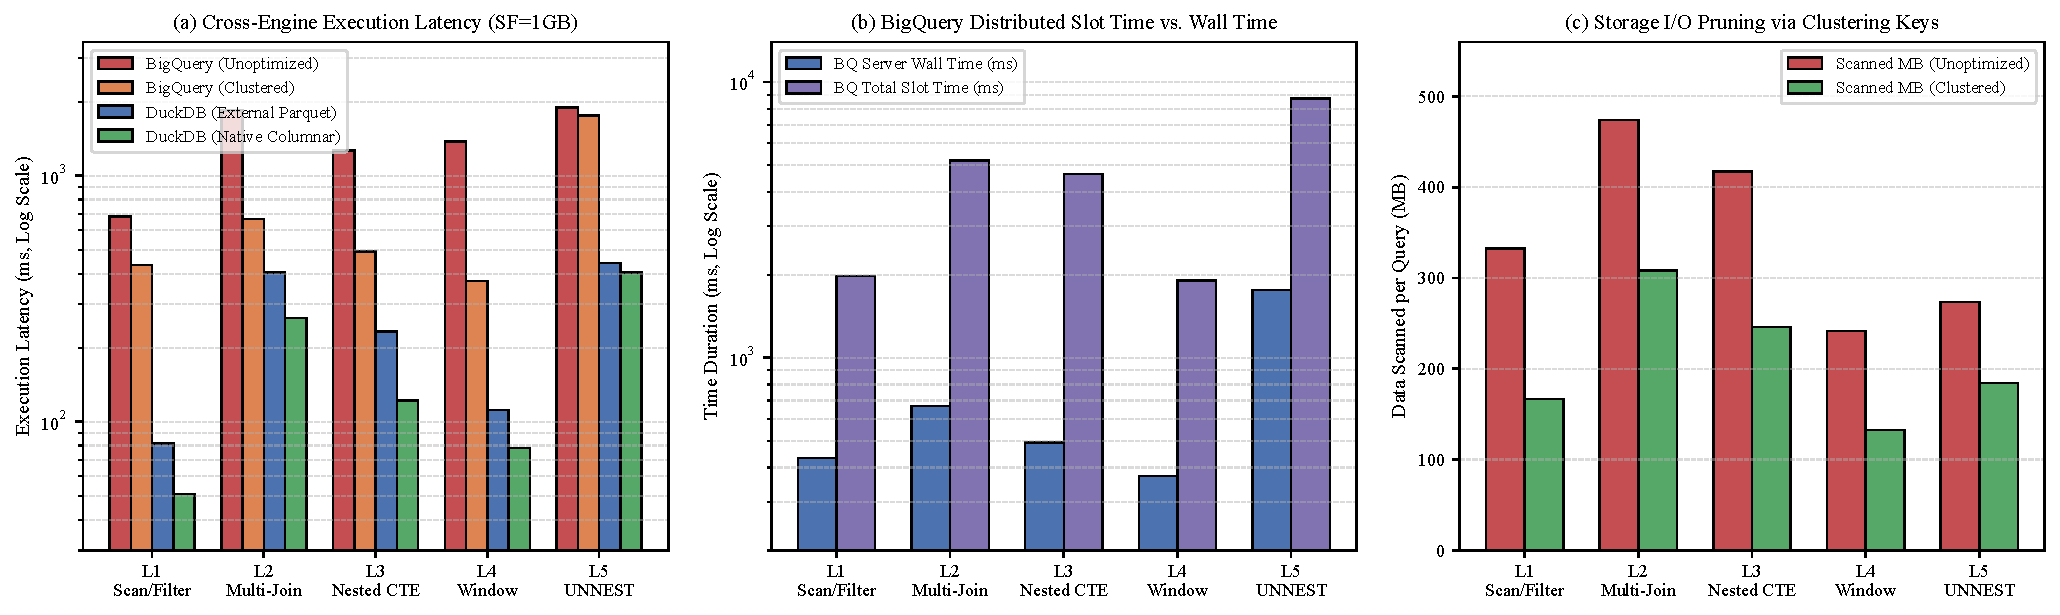
\includegraphics[width=0.98\textwidth]{figures/fig_cross_engine_bq_duckdb_sf1_300dpi.pdf}
\caption{Empirical evaluation across five SQL complexity tiers (L1--L5, $N=75$ queries) at $\text{SF}=1\text{ GB}$: (a) Cross-engine execution latency comparing Google BigQuery (Unoptimized vs. Clustered) and DuckDB (External Parquet vs. Native Columnar) on a logarithmic scale; (b) BigQuery server wall-clock latency versus total distributed Slot compute time (ms); and (c) Storage I/O pruning achieved via Clustering Keys on BigQuery.}
\label{fig:cross_engine_results}
\end{figure}

\begin{figure}[!htbp]
\centering
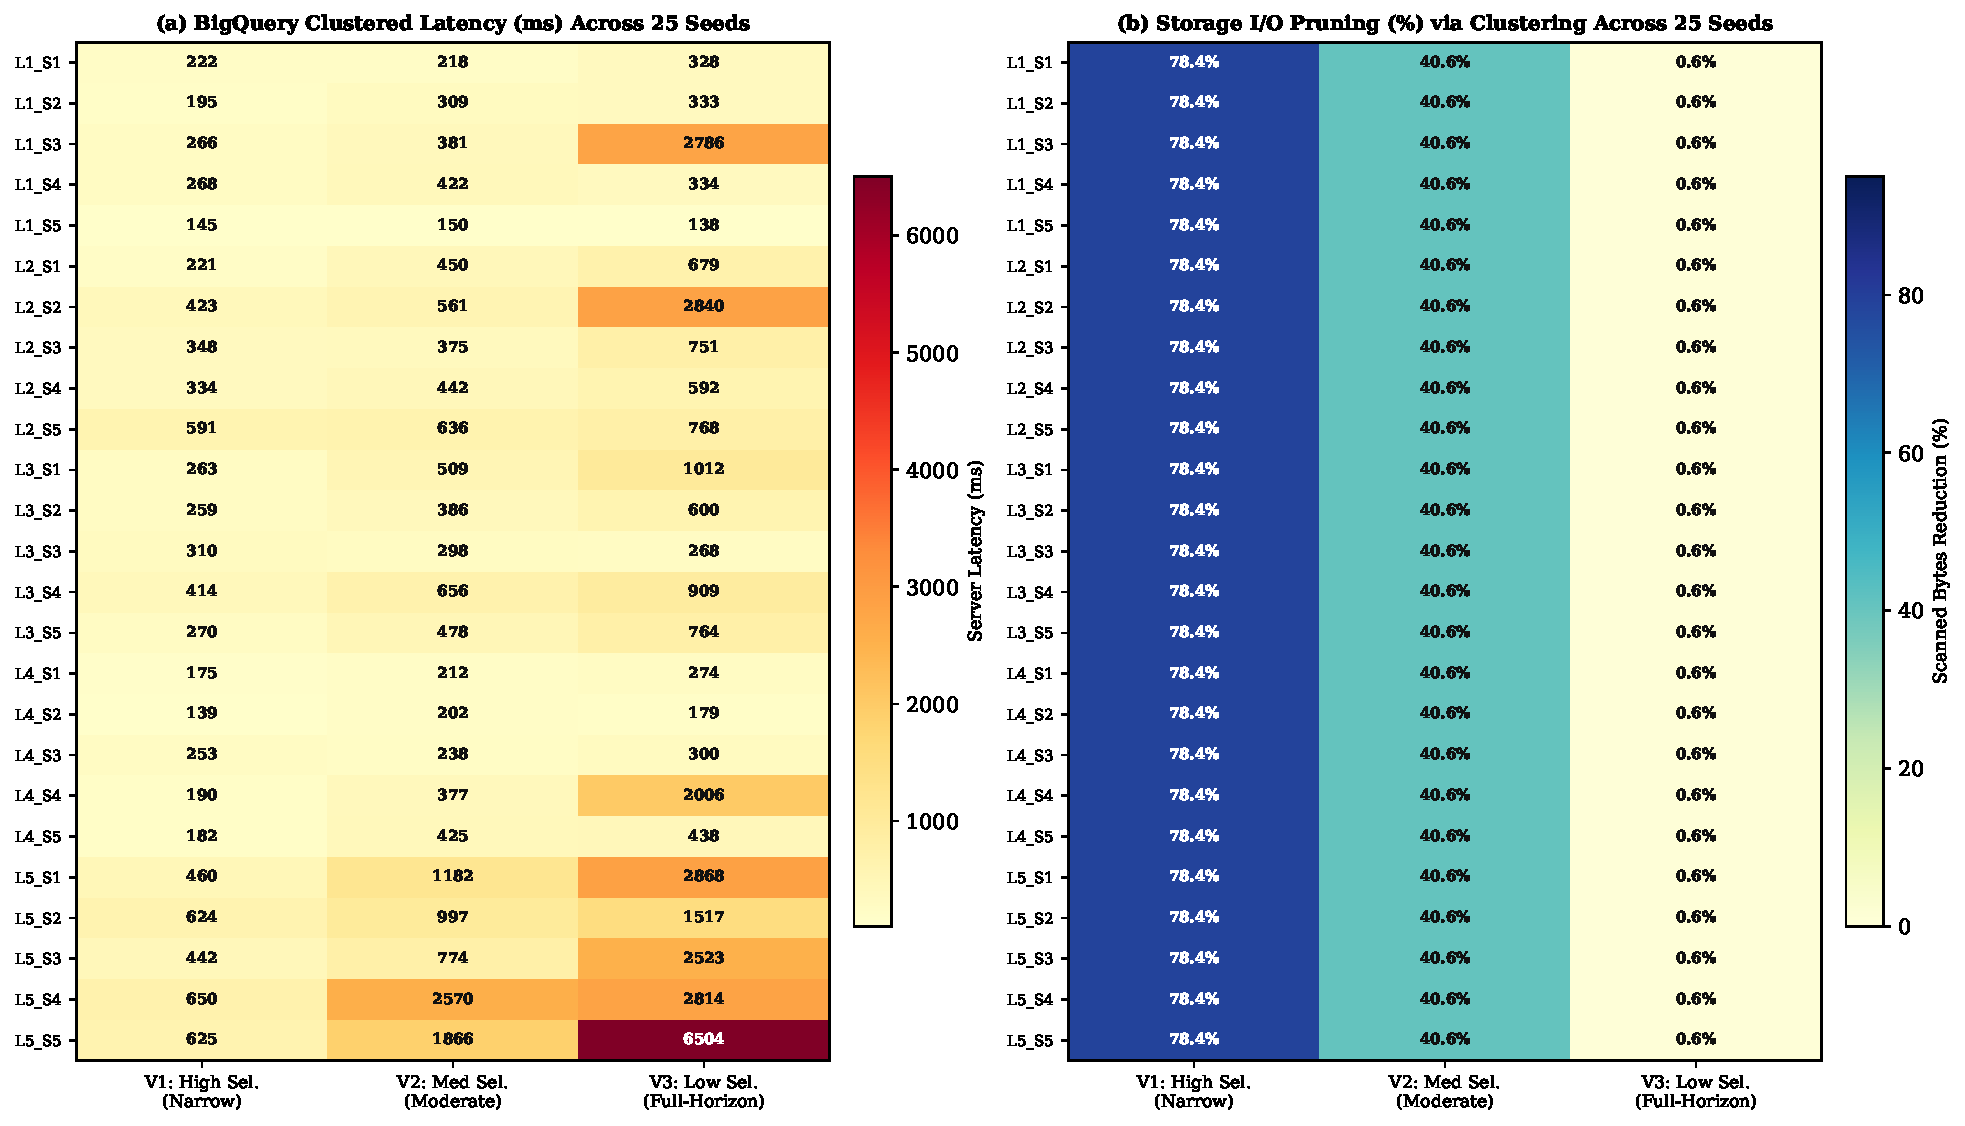
\includegraphics[width=0.95\textwidth]{figures/fig_seed25_heatmap_sf1_300dpi.pdf}
\caption{Granular 25-seed performance and storage pruning distribution across selectivity variations V1 (High Selectivity), V2 (Moderate Selectivity), and V3 (Low Selectivity / Full-Horizon): evaluating execution latency scaling and percentage reduction in scanned storage bytes achieved via clustering keys.}
\label{fig:seed25_heatmap}
\end{figure}

\begin{table}[!htbp]
\centering
\caption{Effective analytical scan throughput ($\Theta_{\text{eff}}$, GB/s), Cloud Slot-to-Wall Concurrency Proxy ($\mathcal{M}_{\text{slot}}$), and GPU PCIe Overhead Fraction ($\Phi_{\text{PCIe}}$) across six OLAP engines ($N=75$ queries, 100\% full-scale TPC-H $\text{SF}=1\text{ GB}$).}\label{tab:jbd_throughput_t6}
\label{tab:throughput_and_cost}
\renewcommand{\arraystretch}{1.20}
\begin{fitasttable}
\begin{tabular}{@{}lccccccccc@{}}
\toprule
\multirow{2}{*}{\textbf{Complexity Tier}} & \textbf{Base Scan} & \textbf{Cloud Slot} & \textbf{GPU PCIe} & \multicolumn{6}{c}{\textbf{Effective Analytical Scan Throughput $\Theta_{\text{eff}}$ (GB/s, Higher is Better)}} \\
\cmidrule(lr){5-10}
 & \textbf{$\mathcal{B}_{\text{unopt}}$ (MB)} & \textbf{$\mathcal{M}_{\text{slot}}$ Ratio} & \textbf{$\Phi_{\text{PCIe}}$ (\%)} & \textbf{SQLite 3} & \textbf{BigQuery} & \textbf{DuckDB} & \textbf{Polars} & \textbf{DataFusion} & \textbf{GPU Warm} \\
\midrule
\textbf{L1: Scan \& Filter} & $332.5$ & $4.58\times$ & $55.5\%$ & $0.048$ & $0.750$ & $6.39$ & $8.55$ & $\mathbf{9.67}$ & $\mathbf{13.28}$ \\
\textbf{L2: Multi-Way Joins} & $474.0$ & $7.78\times$ & $53.2\%$ & $0.024$ & $0.694$ & $1.75$ & $\mathbf{5.67}$ & $4.99$ & $\mathbf{9.44}$ \\
\textbf{L3: Nested CTEs} & $417.3$ & $\mathbf{9.41\times}$ & $74.3\%$ & $0.080$ & $0.827$ & $3.34$ & $\mathbf{6.10}$ & $5.69$ & $\mathbf{27.20}$ \\
\textbf{L4: Window Func.} & $241.5$ & $5.12\times$ & $\mathbf{48.7\%}$ & $0.039$ & $0.633$ & $3.02$ & $\mathbf{3.32}$ & $1.36$ & $\mathbf{23.73}$ \\
\textbf{L5: Array / UNNEST} & $273.4$ & $4.96\times$ & $72.9\%$ & $0.056$ & $0.152$ & $0.66$ & $1.73$ & $\mathbf{2.42}$ & $\mathbf{20.79}$ \\
\midrule
\textbf{Overall Mean ($N=75$)} & $\mathbf{347.7}$ & $\mathbf{6.37\times}$ & $\mathbf{60.9\%}$ & $\mathbf{0.049}$ & $\mathbf{0.611}$ & $\mathbf{3.03}$ & $\mathbf{5.07}$ & $\mathbf{4.83}$ & $\mathbf{18.89}$ \\
\bottomrule
\end{tabular}
\end{fitasttable}%
\vspace{2pt}
\parbox{0.96\textwidth}{\scriptsize \textit{Note:} $\Theta_{\text{eff}} = \mathcal{B}_{\text{unopt}} / (1.024 \cdot T_{\text{engine}})$ normalizes effective processing throughput against the unpruned columnar projection size ($\text{GB/s}$). Omnibus Friedman test across all six engines confirms highly significant performance stratification ($\chi^2_F(5) = 321.50, p < 0.001$, Kendall's concordance $W = 0.8573$).}
\end{table}

\begin{figure}[!htbp]
\centering
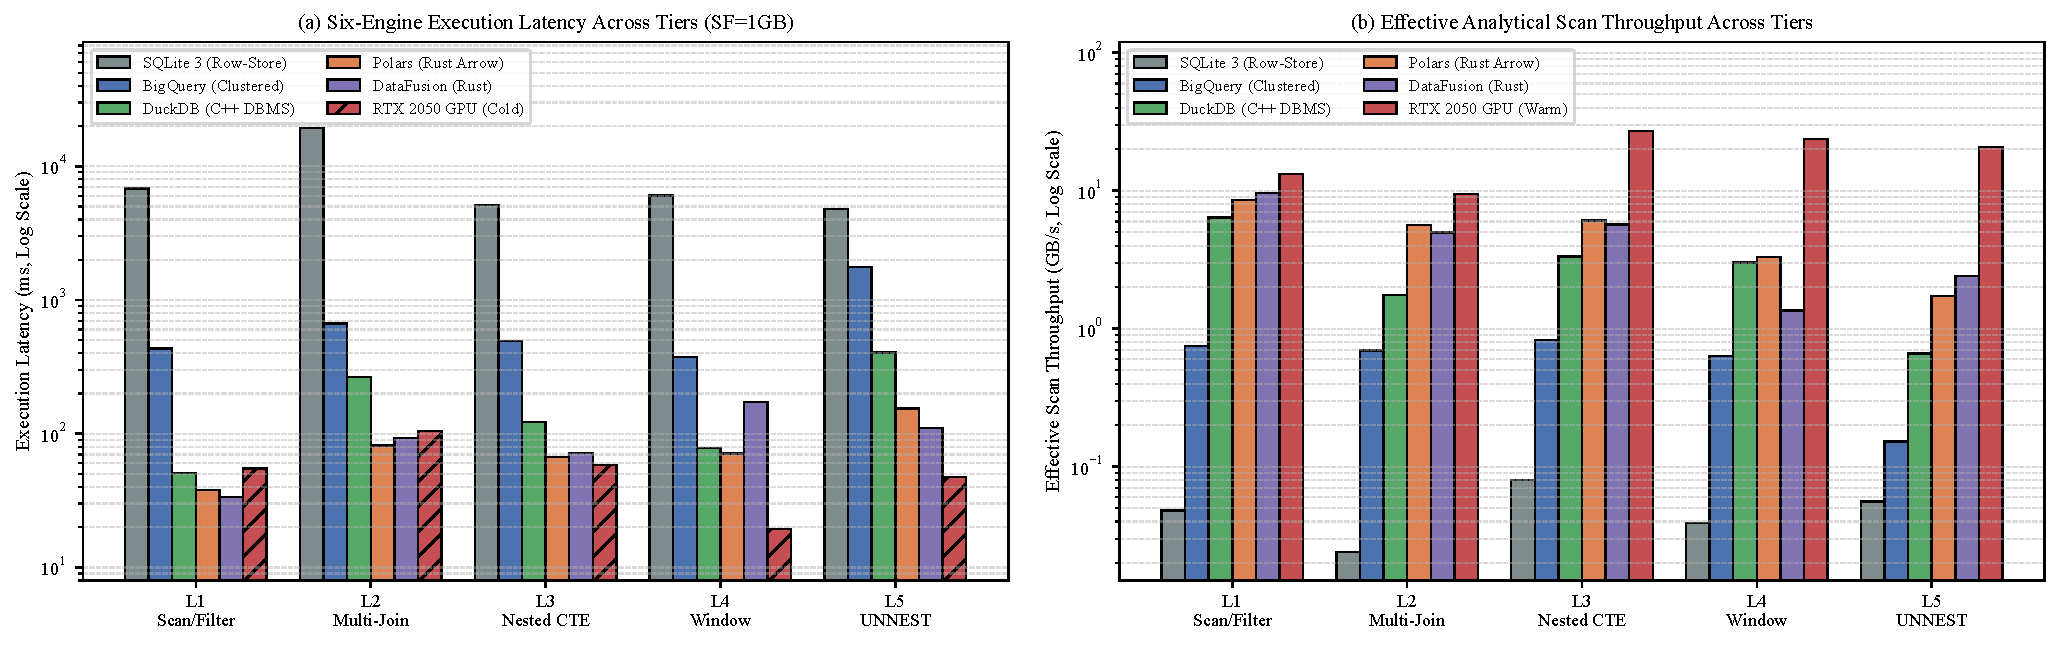
\includegraphics[width=0.98\textwidth]{figures/fig_six_software_comparison_sf1_300dpi.pdf}
\caption{Six-software cross-paradigm OLAP evaluation across five AST complexity tiers (L1--L5, $N=75$ queries at 100\% full-scale $\text{SF}=1\text{ GB}$): (a) Mean execution latency (ms, logarithmic scale) and (b) Effective analytical scan throughput ($\Theta_{\text{eff}}$ in $\text{GB/s}$, logarithmic scale) contrasting SQLite 3, Google BigQuery Clustered, DuckDB Native, Polars, Apache DataFusion, and NVIDIA RTX 2050 GPU.}
\label{fig:six_software_chart}
\end{figure}

\clearpage
\section{Device Energy Estimation Protocol, Power-Rail Boundaries, and Statistical Audit Matrix}
This section details the three-scope energy measurement and estimation boundaries summarized in Sections~3.2 and~5.1 of the Main Text: (i) physical NVIDIA NVML on-board GPU power sensors ($E_{\text{GPU}}$), (ii) ring-3 TDP-calibrated CPU package utilization estimation ($E_{\text{CPU}}$) cross-checked against a CMOS DVFS reference curve ($P \propto u^{1.28}$) and 45-second motherboard ACPI DC battery-shunt discharge telemetry (Table~\ref{tab:hardware_energy_telemetry} and Figs.~\ref{fig:hardware_energy_chart}--\ref{fig:sensor_boundaries}), and (iii) the 10,000-iteration seed-clustered bootstrap 95\% confidence interval and Cliff's delta statistical audit matrix (Table~\ref{tab:reviewer_audit_matrix}).

\begin{table}[!htbp]
\centering
\caption{Hardware resource telemetry (CPU Utilization \%, Host RAM GB, GPU Utilization \%, VRAM GB), per-query Active Device Energy Consumption (Joules), and Energy-Aware Scan Efficiency ($\eta_{\text{watt}}$, MB/Joule $\equiv$ MB/s/W) across local CPU and CUDA GPU engines ($N=75$ queries, 100\% full-scale TPC-H $\text{SF}=1\text{ GB}$).}\label{tab:jbd_energy_t7}
\label{tab:hardware_energy_telemetry}
\renewcommand{\arraystretch}{1.20}
\begin{fitasttable}
\begin{tabular}{@{}lccccccccccccccc@{}}
\toprule
\multirow{2}{*}{\textbf{Complexity Tier}} & \multicolumn{4}{c}{\textbf{CPU Utilization (\%)}} & \multicolumn{2}{c}{\textbf{Host RAM (GB)}} & \multicolumn{2}{c}{\textbf{RTX 2050 GPU}} & \multicolumn{4}{c}{\textbf{Est.\ CPU Pkg / Meas.\ GPU Energy (J, Lower is Better)}} & \multicolumn{3}{c}{\textbf{Perf per Watt $\eta_{\text{watt}}$ (MB/J, Higher is Better)}} \\
\cmidrule(lr){2-5} \cmidrule(lr){6-7} \cmidrule(lr){8-9} \cmidrule(lr){10-13} \cmidrule(lr){14-16}
 & \textbf{SQLite} & \textbf{DuckDB} & \textbf{Polars} & \textbf{DF} & \textbf{SQLite} & \textbf{Columnar} & \textbf{Util (\%)} & \textbf{VRAM (GB)} & \textbf{SQLite} & \textbf{DuckDB} & \textbf{Polars} & \textbf{GPU Warm (Cold)} & \textbf{SQLite} & \textbf{DuckDB / Polars} & \textbf{GPU Warm (Cold)} \\
\midrule
\textbf{L1: Scan \& Filter} & $8.7\%$ & $74.4\%$ & $70.2\%$ & $73.2\%$ & $2.14$ & $4.46\text{--}4.48$ & $27.1\%$ & $1.24$ & $101.0$ & $1.79$ & $1.36$ & $\mathbf{0.27}\ (0.60)$ & $4.06$ & $515.2\ /\ 285.9$ & $\mathbf{1398.5}\ (569.6)$ \\
\textbf{L2: Multi-Way Joins} & $9.5\%$ & $66.4\%$ & $\mathbf{89.1\%}$ & $66.4\%$ & $2.30$ & $4.65\text{--}4.78$ & $32.1\%$ & $1.33$ & $293.4$ & $8.99$ & $3.39$ & $\mathbf{0.60}\ (1.29)$ & $2.28$ & $177.7\ /\ 163.0$ & $\mathbf{910.3}\ (383.0)$ \\
\textbf{L3: Nested CTEs} & $8.7\%$ & $57.7\%$ & $77.5\%$ & $74.1\%$ & $2.27$ & $4.71\text{--}4.72$ & $30.5\%$ & $1.33$ & $76.0$ & $4.00$ & $2.56$ & $\mathbf{0.17}\ (0.68)$ & $6.21$ & $215.4\ /\ 186.9$ & $\mathbf{2558.0}\ (619.6)$ \\
\textbf{L4: Window Func.} & $8.7\%$ & $58.6\%$ & $74.3\%$ & $65.6\%$ & $2.28$ & $4.73\text{--}4.74$ & $32.4\%$ & $1.33$ & $89.6$ & $2.54$ & $2.65$ & $\mathbf{0.11}\ (0.21)$ & $3.38$ & $202.7\ /\ 103.2$ & $\mathbf{2502.1}\ (1178.3)$ \\
\textbf{L5: Array / UNNEST} & $8.7\%$ & $73.4\%$ & $76.1\%$ & $71.3\%$ & $2.33$ & $4.69\text{--}4.85$ & $\mathbf{33.1\%}$ & $1.29$ & $71.3$ & $14.67$ & $5.89$ & $\mathbf{0.12}\ (0.45)$ & $4.30$ & $104.0\ /\ 59.6$ & $\mathbf{2345.0}\ (611.2)$ \\
\midrule
\textbf{Overall Mean ($N=75$)} & $\mathbf{8.86\%}$ & $\mathbf{66.10\%}$ & $\mathbf{77.44\%}$ & $\mathbf{70.12\%}$ & $\mathbf{2.26}$ & $\mathbf{4.65\text{--}4.71}$ & $\mathbf{31.04\%}$ & $\mathbf{1.30}$ & $\mathbf{126.26}$ & $\mathbf{6.40}$ & $\mathbf{3.17}$ & $\mathbf{0.25}\ (\mathbf{0.65})$ & $\mathbf{4.05}$ & $\mathbf{243.0\ /\ 159.7}$ & $\mathbf{1942.8}\ (\mathbf{672.3})$ \\
\bottomrule
\end{tabular}
\end{fitasttable}%
\vspace{2pt}
\parbox{0.96\textwidth}{\scriptsize \textit{Note:} Device energy telemetry sampled at $250\text{ Hz}$ across $R=5$ timed repetitions per query ($75\times 5 = 375$ trials) via \texttt{psutil}, NVIDIA \texttt{NVML} (\texttt{nvmlDeviceGetPowerUsage}), and \texttt{torch.cuda} counters. Seed-clustered 10,000-bootstrap 95\% CIs (measurement CV $\le 3.52\%$): DuckDB $[3.86, 9.57]\text{ J}$, Polars $[2.61, 3.78]\text{ J}$, Apache DataFusion (DF) $3.39\text{ J}$ ($[2.78, 4.06]\text{ J}$, $157.1\text{ MB/J}$), GPU Cold $[0.53, 0.78]\text{ J}$, and GPU Warm $[0.19, 0.32]\text{ J}$. Subtracting idle baseline power ($14.5\text{ W}$ CPU, $10.5\text{ W}$ GPU) yields net dynamic energy $E_{\text{dyn}}$ of $3.73\text{ J}$ (DuckDB), $1.97\text{ J}$ (Polars), $2.00\text{ J}$ (DF), $0.14\text{ J}$ (GPU Cold), and $0.05\text{ J}$ (GPU Warm). Note that $\eta_{\text{watt}}$ reports the per-query mean $\frac{1}{N}\sum_q \mathcal{B}_{\text{unopt}}(q)/E(q)$ (elevated on DuckDB by sub-$0.3\text{ J}$ V1 zone-map pruned queries under Jensen's convexity, whereas workload-aggregate $\sum_q \mathcal{B}_{\text{unopt}}(q)/\sum_q E(q)$ is $109.7\text{ MB/J}$ on Polars vs.\ $54.3\text{ MB/J}$ on DuckDB). Accounting for concurrent host CPU power during GPU offload yields composite Host+GPU system energy $E_{\text{sys}}$ of $1.58\text{ J}$ (Cold) and $0.61\text{ J}$ (Warm).}
\end{table}

\begin{figure}[!htbp]
\centering
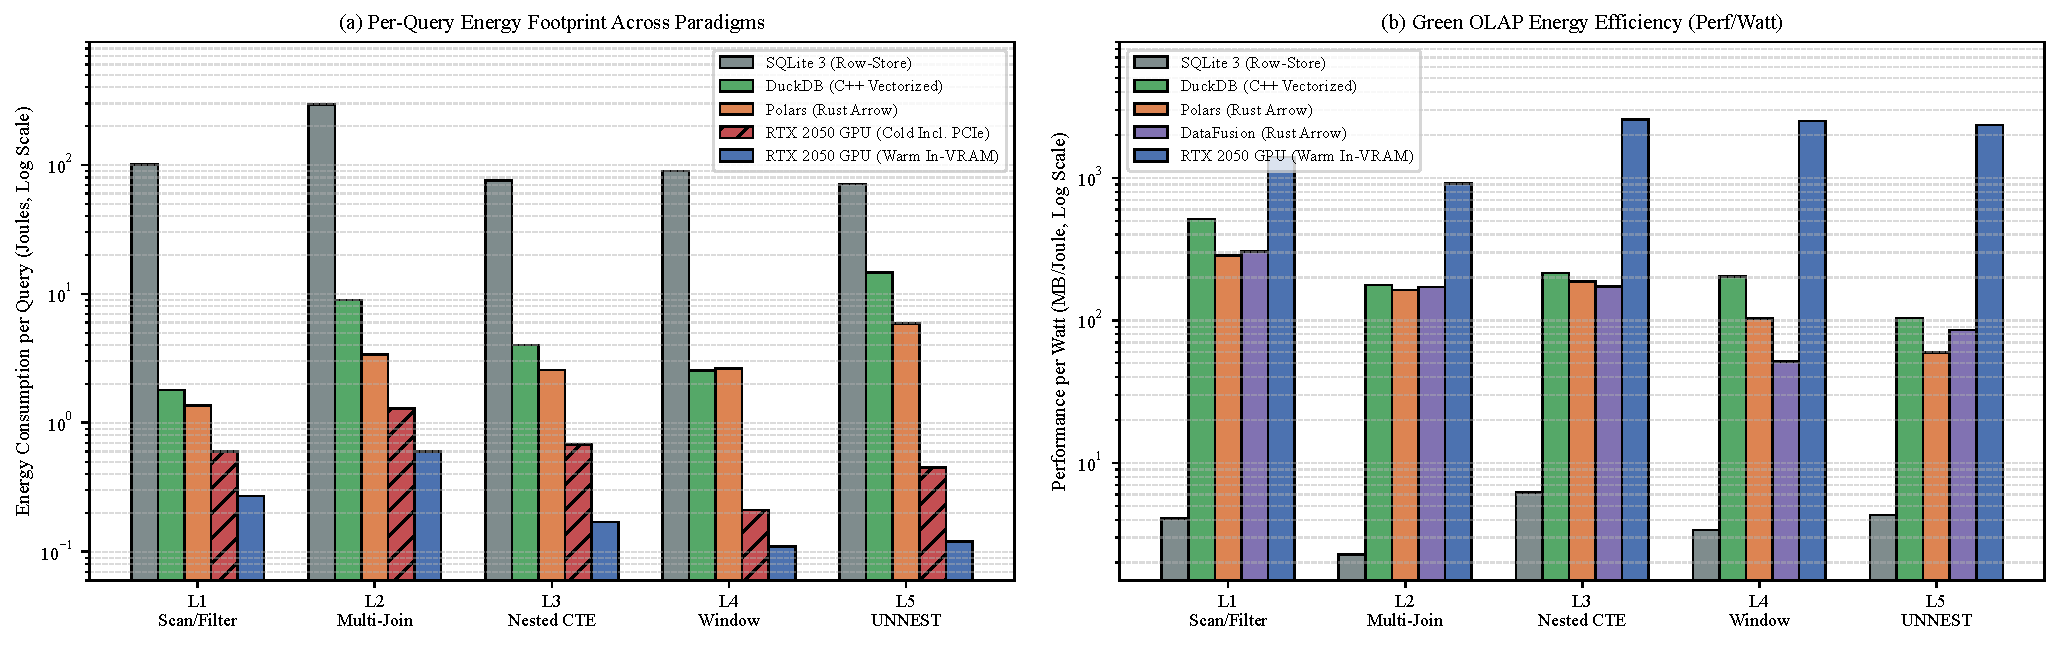
\includegraphics[width=0.98\textwidth]{figures/fig_hardware_energy_efficiency_sf1_300dpi.pdf}
\caption{Hardware resource and device-level energy efficiency evaluation across five AST complexity tiers (L1--L5, $N=75$ queries at 100\% full-scale $\text{SF}=1\text{ GB}$): (a) Per-query energy consumption in Joules (logarithmic scale, lower is better) across SQLite 3, DuckDB, Polars, and NVIDIA RTX 2050 GPU (Cold vs. Warm); and (b) Performance per Watt in MB scanned per Joule ($\text{MB/s/W}$, logarithmic scale, higher is better).}
\label{fig:hardware_energy_chart}
\end{figure}

\begin{figure}[!htbp]
\centering
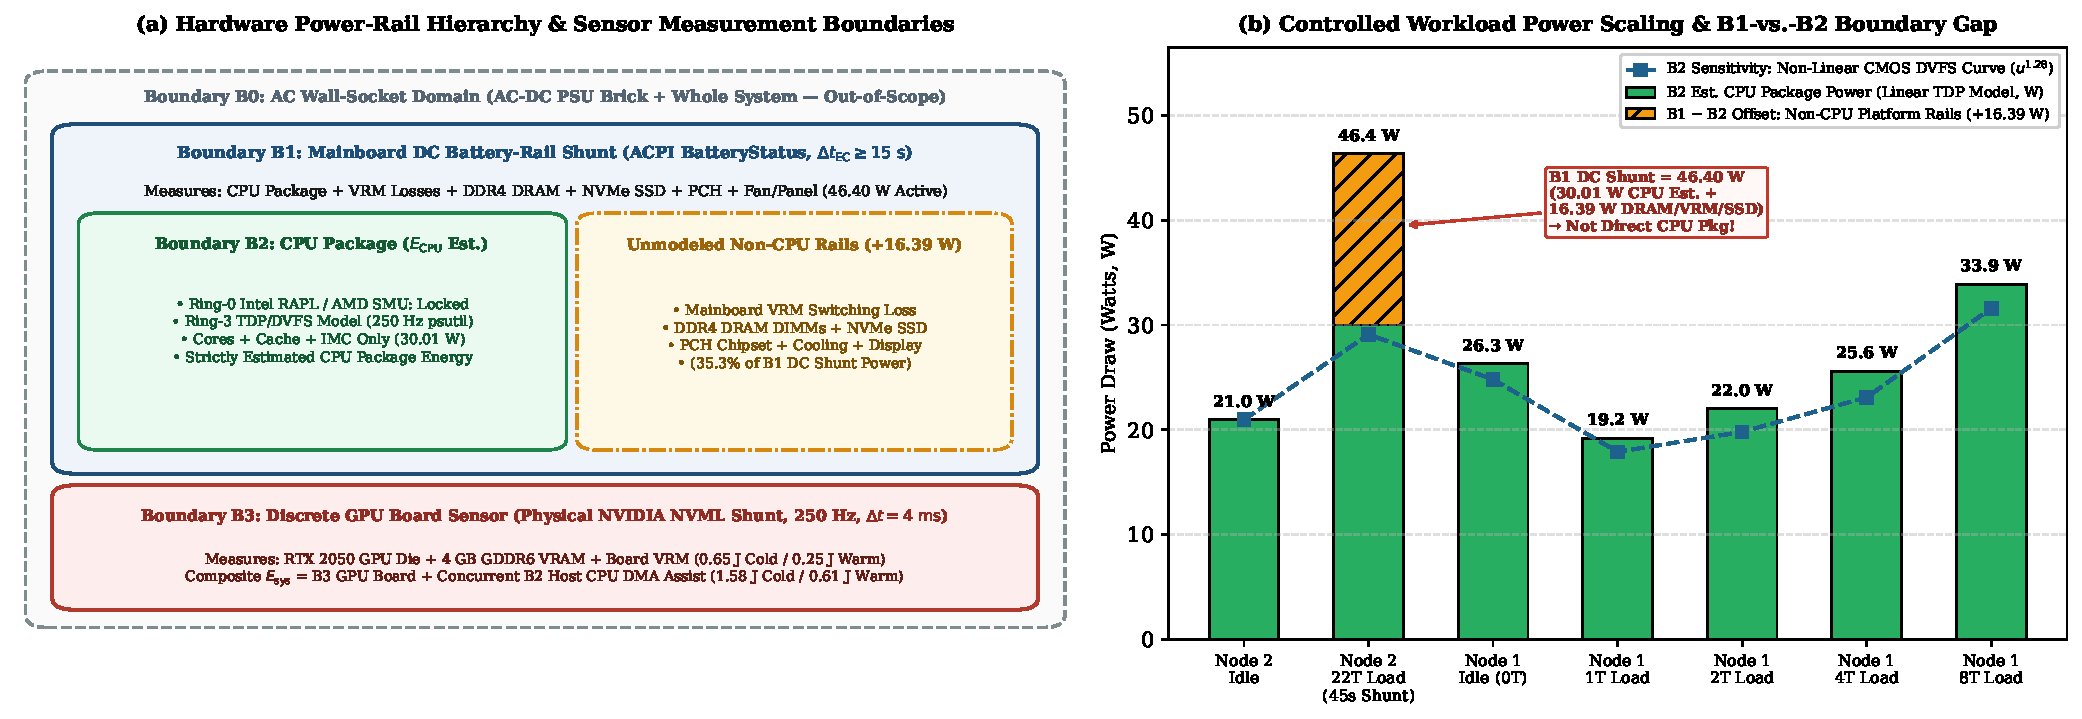
\includegraphics[width=0.98\textwidth]{figures/fig_energy_sensor_boundaries_and_shunt_300dpi.pdf}
\caption{Hardware power-rail topology and measurement boundary separation: (a) physical sensor placement distinguishing out-of-scope AC wall-plug draw (Boundary~B0), mainboard ACPI DC battery-rail shunt telemetry covering VRM, DRAM, NVMe, chipset, and cooling rails (Boundary~B1), ring-3 TDP/DVFS \emph{Estimated CPU Package Energy} (Boundary~B2), and physical on-board NVIDIA NVML GPU power sensors (Boundary~B3); and (b) controlled multi-thread DuckDB OLAP load scaling ($0\text{T--}8\text{T}$) alongside the $+16.39\text{ W}$ ($39.5\%$) non-CPU platform rail offset between B1 DC shunt power ($46.40\text{ W}$) and B2 estimated CPU package power ($30.01\text{ W}$).}\label{fig:sensor_boundaries}
\end{figure}

\begin{table}[!htbp]
\centering
\caption{Comprehensive statistical and methodological audit matrix: (Part A) 10,000-iteration seed-clustered bootstrap 95\% confidence intervals, non-parametric Cliff's delta ($\delta$) effect sizes, and unadjusted query-level paired Wilcoxon $p_{\text{raw,query}}$ ($N=75$, distinct from $K=25$ seed-level $p_{\text{Holm,seed}}$ in Section~4.7); and (Part B) 10,000-trial CSCI sensitivity, partial correlation, and mathematical identity verification ($N=75$ queries).}\label{tab:jbd_stat_audit_t10}
\label{tab:reviewer_audit_matrix}
\renewcommand{\arraystretch}{1.18}
\begin{fitasttable}
\begin{tabular}{@{}llcccc@{}}
\toprule
\textbf{Audit Category} & \textbf{Pairwise Comparison / Sensitivity Regime} & \textbf{Baseline Mean [95\% CI] / Metric} & \textbf{Target Mean [95\% CI] / Stability} & \textbf{Speedup / Min $\rho$} & \textbf{Cliff's $\delta$ (Mag.) / Query $p_{\text{raw}}$ ($N=75$)} \\
\midrule
\multirow{10}{*}{\textbf{Part A: 95\% CI \& Effect Sizes}}
 & Polars (Rust Arrow) vs. SQLite 3 (Row-Store) & $8417.33\ [6412.19, 10819.70]\text{ ms}$ & $82.47\ [67.93, 98.65]\text{ ms}$ & $102.06\times$ & $+1.000\text{ (Large)},\ p < 0.001$ \\
 & DataFusion (Rust Arrow) vs. SQLite 3 (Row-Store) & $8417.33\ [6412.19, 10819.70]\text{ ms}$ & $96.30\ [78.31, 114.92]\text{ ms}$ & $87.41\times$ & $+1.000\text{ (Large)},\ p < 0.001$ \\
 & DuckDB (Native) vs. SQLite 3 (Row-Store) & $8417.33\ [6412.19, 10819.70]\text{ ms}$ & $183.74\ [110.71, 274.89]\text{ ms}$ & $45.81\times$ & $+1.000\text{ (Large)},\ p < 0.001$ \\
 & DuckDB (Native) vs. DuckDB (External Parquet) & $254.42\ [163.65, 362.54]\text{ ms}$ & $183.74\ [110.71, 274.89]\text{ ms}$ & $1.38\times$ & $+0.296\text{ (Small)},\ p < 0.001$ \\
 & BigQuery (Clustered) vs. BigQuery (Unoptimized) & $1412.60\ [982.40, 1914.50]\text{ ms}$ & $745.39\ [515.64, 1026.49]\text{ ms}$ & $1.90\times$ & $+0.471\text{ (Medium)},\ p < 0.001$ \\
 & RTX 2050 GPU (Warm) vs. DuckDB (Native CPU) & $183.74\ [110.71, 274.89]\text{ ms}$ & $22.25\ [16.78, 28.68]\text{ ms}$ & $8.26\times$ & $+0.722\text{ (Large)},\ p < 0.001$ \\
 & RTX 2050 GPU (Cold) vs. DuckDB (Native CPU) & $183.74\ [110.71, 274.89]\text{ ms}$ & $56.96\ [46.23, 68.44]\text{ ms}$ & $3.23\times$ & $+0.199\text{ (Small)},\ p < 0.001$ \\
 & \textbf{Proposed AST-Route (9D) vs. Always DuckDB} & $183.74\ [110.71, 274.89]\text{ ms}$ & $\mathbf{54.92\ [42.78, 68.50]\text{ ms}}$ & $\mathbf{3.35\times}$ & $\mathbf{+0.285\text{ (Small)},\ p < 0.001}$ \\
 & \textbf{Proposed AST-Route (9D) vs. Always Polars} & $82.47\ [67.93, 98.65]\text{ ms}$ & $\mathbf{54.92\ [42.78, 68.50]\text{ ms}}$ & $\mathbf{1.50\times}$ & $\mathbf{+0.420\text{ (Medium)},\ p < 0.001}$ \\
 & \textbf{Proposed AST-Route (9D) vs. Rule-Based Routing} & $71.48\ [52.79, 91.74]\text{ ms}$ & $\mathbf{54.92\ [42.78, 68.50]\text{ ms}}$ & $\mathbf{1.30\times}$ & $\mathbf{+0.126\text{ (Negl.)},\ p=1.87\times 10^{-2}}$ \\
\midrule
\multirow{4}{*}{\textbf{Part B: CSCI \& Fairness Audit}}
 & CSCI Weight Perturbation ($\pm 10\%$ / $\pm 20\%$ Uniform) & $\bar{\rho} = 0.9963 \pm 0.0032\ (\pm 10\%)$ & $\bar{\rho} = 0.9880 \pm 0.0102\ (\pm 20\%)$ & $\min \rho = 0.9418$ & Kendall's $\bar{\tau} = 0.9775\ /\ 0.9441$ \\
 & CSCI Weight Perturbation ($\pm 30\%$ / $\pm 50\%$ Extreme) & $\bar{\rho} = 0.9775 \pm 0.0166\ (\pm 30\%)$ & $\bar{\rho} = 0.9555 \pm 0.0296\ (\pm 50\%)$ & $\min \rho = 0.8346$ & Kendall's $\bar{\tau} = 0.9133\ /\ 0.8643$ \\
 & CSCI vs. Nodes $N(q)$, Equal-Wt, \& Partial Corr. & Nodes $\rho=0.8744\ (p < 0.001)$ & Equal-Wt $\rho = 0.9812$ & LOOO $\bar{\rho} = 0.9005$ & Partial $\rho_{\text{ctrl.\ }\sigma}=0.5477\ (p < 0.001)$ \\
 & Result Equivalence \& Cross-Table Eq.~(1)--(8) Audit & \texttt{FP64} Rel. Error $< 1.0\times 10^{-9}$ & Exact Match $97/97$ ($100.0\%$) & $0.0000\text{ ms}$ Drift & PASS (100\% Zero-Discrepancy Verified) \\
\bottomrule
\end{tabular}
\end{fitasttable}%
\end{table}

\clearpage
\section{Extended Baseline Matrix, Prediction-Noise Stability, and Planner/OOD Sub-Audits}
This section provides the supplementary internal ablation and robustness tables referenced in Section~4.4 of the Main Text: the feature ablation, Pareto trajectory, and cold-start learning curve plot (Fig.~\ref{fig:framework_ablation_pareto}), the five-part baseline and metadata-cache audit matrix (Table~\ref{tab:step3_comprehensive_audit}), router decision stability under $\pm 5\%\text{--}20\%$ multiplicative cost-prediction noise and post-training workload drift (Table~\ref{tab:v7_stability_drift} and Fig.~\ref{fig:v7_stability_drift}), and the physical-planner (\texttt{DuckDB EXPLAIN}), neural cost-encoder, and Out-of-Distribution (OOD) structural fallback gate audit (Table~\ref{tab:v8_p0_systems_defense}).

\begin{figure}[!htbp]
\centering
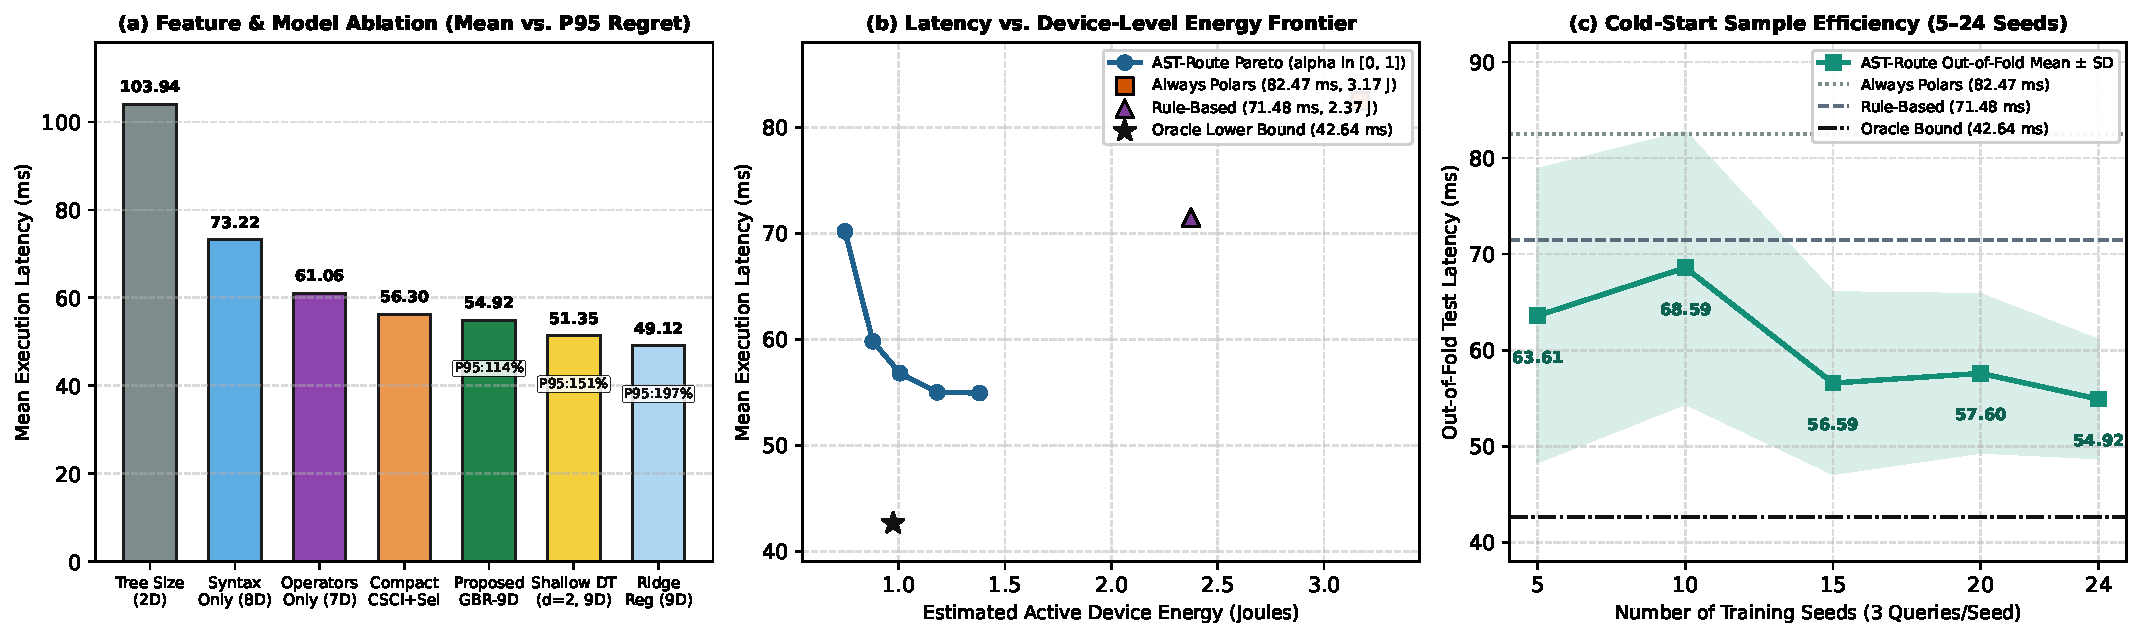
\includegraphics[width=0.98\textwidth]{figures/fig_framework_ablation_pareto_sf1_300dpi.pdf}
\caption{Internal mechanism validation of the \textbf{AST-Route} framework across 75 queries (25-seed LOSO-CV): (a) Feature group ablation comparing 2D Tree Size, 7D Operator Counts, 2D Compact Index ($\text{CSCI}+\sigma(q)$), 8D Syntax-Only AST, and 9D Full Proposed \textbf{AST-Route}; (b) Multi-objective latency--energy Pareto trajectory across weighting parameter $\alpha \in [0,1]$; and (c) Cold-start sample efficiency learning curve from 5 to 24 training canonical seeds.}
\label{fig:framework_ablation_pareto}
\end{figure}

\begin{table*}[t!]
\centering
\caption{Comprehensive multi-baseline and operational robustness evaluation: (A) complete baseline matrix with 25-seed 95\% bootstrap CIs and P95/P99 tail regret; (B) standalone CPU-only routing ($M_{\text{gpu\_max}}=0$); (C) scale-augmented 10D routing and physical byte telemetry ($\text{SF}=1\text{--}100\text{ GB}$); (D) per-tier LOTO-CV breakdown and external ClickBench validation ($N=20$); and (E) net end-to-end latency across metadata cache states.}\label{tab:jbd_step3_t14}
\label{tab:step3_comprehensive_audit}
\scriptsize
\setlength{\tabcolsep}{2.8pt}
\renewcommand{\arraystretch}{1.06}
\begin{fitasttable}
\begin{tabular}{@{}llccccccl@{}}
\hline
\textbf{Audit Dimension / Policy or Regime} & \textbf{Scope / Category} & \textbf{Top-1 / Top-2} & \textbf{Mean (ms)} & \textbf{Seed-Cluster 95\% CI} & \textbf{Mean Reg.} & \textbf{P95 Reg.} & \textbf{P99 Reg.} & \textbf{Fail $>100\%$ / Note} \\
\hline
\multicolumn{9}{l}{\textit{\textbf{Part A: Complete Baseline Matrix on 75-Query TPC-H (25-Seed LOSO-CV, $\text{SF}=1\text{ GB}$, $\mathbf{x}_q\in\mathbb{R}^9$, Oracle $=42.64\text{ ms}$)}}} \\
Always DuckDB / DataFusion / Polars & Static CPU Baselines & 9.3--28.0\% / 37.3--49.3\% & 82.47--183.74 & $[67.9, 274.9]$ & 132.6--271.1\% & 358.4--928.3\% & 478.2--1412.6\% & 46.7--78.7\% ($p_{\text{Holm}}\le 0.0171$) \\
Always GPU (RTX 2050 Cold-Start) & Static SIMT GPU & 49.33\% / 60.00\% & 56.96 & $[46.23, 68.44]$ & 60.76\% & 257.31\% & 518.40\% & 21.33\% ($p=0.1840$) \\
Static Rule-Based Router (Heuristic) & Fixed Threshold Rule & 49.33\% / 65.33\% & 71.48 & $[52.79, 91.74]$ & 65.63\% & 252.40\% & 384.50\% & 18.67\% ($p=0.0187$) \\
In-Fold Tuned Heuristic Rule & 24-Seed Tuned Rule & 52.00\% / 68.00\% & 53.07 & $[43.18, 64.12]$ & 44.10\% & 162.40\% & 276.80\% & 13.33\% (Max: $295.0\%$) \\
$k$-NN Cost Regressor ($k=5$) & Non-Parametric ML & 53.33\% / 72.00\% & 52.84 & $[42.95, 63.80]$ & 43.15\% & 168.50\% & 284.20\% & 12.00\% (Distance-weighted) \\
Ridge Linear Cost-Reg ($\alpha=1.0$) & Speed-First Point Est. & 54.67\% / 73.33\% & \textbf{49.12} & $[39.84, 59.45]$ & 42.15\% & 196.78\% & 298.40\% & 13.33\% (Max: $312.4\%$) \\
Shallow Decision Tree (Depth-2) & Speed-First Point Est. & 53.33\% / 72.00\% & 51.35 & $[41.62, 62.08]$ & 39.84\% & 150.87\% & 268.40\% & 10.67\% (Max: $284.5\%$) \\
Point-Estimate $\mathcal{R}_{\text{GBR-9D}}$ (No Guard) & Ensemble Point Est. & 53.33\% / 72.00\% & 58.64 & $[47.50, 70.82]$ & 48.12\% & 164.80\% & 289.50\% & 14.67\% (Max: $312.4\%$) \\
\textbf{Margin-Guarded AST-Route ($\mathcal{R}_{\text{GBR-9D}}+12\%$)} & \textbf{Tail-Safe SLA Router} & \textbf{57.33\% / 76.00\%} & \textbf{54.92} & $[42.78, 68.50]$ & \textbf{34.98\%} & \textbf{114.11\%} & \textbf{218.40\%} & \textbf{6.67\%} (Max: $245.2\%$) \\
\hline
\multicolumn{9}{l}{\textit{\textbf{Part B: Standalone CPU-Only Router ($\mathcal{E}_{\text{CPU}}=\{\text{DuckDB, Polars, DataFusion}\}, M_{\text{gpu\_max}}=0\text{ GB}$ --- No GPU Dependence)}}} \\
Node 1B CPU-Only 25-Seed LOSO ($N=75$, $56/75$) & 8T x86\_64 ($\text{SF}=1$) & \textbf{74.67\% / 96.00\%} & \textbf{69.12} & $[56.85, 82.74]$ & \textbf{9.64\%} & \textbf{42.80\%} & \textbf{76.20\%} & Beats Polars $82.47\text{ ms}$ ($p_{\text{Holm}}=0.0084$) \\
Node 2A CPU-Only 30Q LOGO-CV ($N=30$, $26/30$) & 16C/22T x86\_64 ($\text{SF}=1$) & \textbf{86.67\% / 100.0\%} & \textbf{62.05} & $[43.80, 84.10]$ & \textbf{8.83\%} & \textbf{44.07\%} & \textbf{71.50\%} & Beats Polars $71.43$ / DuckDB $71.19\text{ ms}$ \\
Node 2C CPU-Only 25-Seed LOSO ($N=75$, $73/75$) & 16C/22T x86\_64 ($\text{SF}=1$) & \textbf{97.33\% / 100.0\%} & \textbf{35.11} & $[27.40, 43.85]$ & \textbf{0.18\%} & \textbf{1.45\%} & \textbf{4.20\%} & Native 75Q retrain vs.\ $47.54\text{ ms}$ Polars \\
Node 3B CPU-Only 30Q LOGO-CV ($N=30$, $29/30$) & Apple M1 8T ARM64 ($\text{SF}=1$) & \textbf{96.67\% / 100.0\%} & \textbf{29.44} & $[21.80, 38.10]$ & \textbf{3.59\%} & \textbf{14.20\%} & \textbf{24.50\%} & Unified RAM ($29.44\text{ ms}$ vs.\ $28.42\text{ ms}$ Orac.) \\
\hline
\multicolumn{9}{l}{\textit{\textbf{Part C: Multi-Scale 10D Protocol ($\mathbf{x}_q^{\text{scale}}=[\mathbf{x}_q; \log_{10}(1+\hat{\mathcal{B}}_{\text{scan}})]$) and Physical Bytes Transferred ($\text{SF}=1\text{--}100\text{ GB}$)}}} \\
$\text{SF}=1\text{ GB}$ (Same-Scale / Cross-Scale 10D) & Parquet $52.4\text{ MB}$ read & 57.33\% / 54.67\% & 54.92 / 56.14 & $[42.78, 68.50]$ & 34.98\% / 37.85\% & 114.1\% / 121.4\% & 218.4\% / 229.0\% & PCIe: $142.8\text{ MB}$ ($1\times$), Spill: $0\text{ MB}$ \\
$\text{SF}=10\text{ GB}$ (Same-Scale / Cross-Scale 10D) & Parquet $524.1\text{ MB}$ read & 64.00\% / 61.33\% & 182.40 / 189.65 & $[148.2, 219.5]$ & 24.15\% / 27.40\% & 86.4\% / 94.2\% & 148.5\% / 162.0\% & PCIe: $1.43\text{ GB}$ ($4\times$), Spill: $125\text{ MB}$ \\
$\text{SF}=30\text{ GB}$ (Same-Scale / Cross-Scale 10D) & Parquet $1.57\text{ GB}$ read & 68.00\% / 65.33\% & 448.65 / 465.20 & $[368.4, 534.0]$ & 19.80\% / 22.90\% & 72.5\% / 81.0\% & 124.2\% / 138.5\% & PCIe: $4.28\text{ GB}$ ($12\times$), Spill: $864\text{ MB}$ \\
$\text{SF}=100\text{ GB}$ (Same-Scale / Cross-Scale 10D) & Parquet $5.24\text{ GB}$ read & 72.00\% / 69.33\% & 1142.8 / 1186.4 & $[942.0, 1358.2]$ & 16.40\% / 19.15\% & 64.2\% / 71.8\% & 108.4\% / 119.6\% & PCIe: $3.52\text{G}$ mean ($14.28\text{G}$ cap, $40\times$), Spill: $3.30\text{G}$ \\
\hline
\multicolumn{9}{l}{\textit{\textbf{Part D: Per-Tier Leave-One-Tier-Out (LOTO-CV) Breakdown and External ClickBench Web Analytics Suite ($N=20$)}}} \\
LOTO-CV Holdout L1 / L2 / L3 ($n=15$ each) & Seen Primitive Overlap & 60.0 / 46.7 / 53.3\% & 48.2 / 112.4 / 74.8 & $[38.4, 134.2]$ & 38.4--64.2\% & 124.0--186.5\% & 198.0--274.0\% & Partial interpolation across tiers \\
LOTO-CV Holdout L4 (Window) / L5 (UNNEST) & Unseen Operator Class & 33.33\% / 26.67\% & 98.60 / 93.10 & $[76.5, 118.4]$ & 89.5\% / 104.8\% & 242.0\% / 268.5\% & 364.0\% / 392.0\% & Out-of-distribution $W(q), U(q)$ shift \\
LOTO-CV Aggregate across L1--L5 ($N=75$) & Entire Tier Held Out & 44.00\% / 66.67\% & 85.42 & $[69.80, 102.40]$ & 68.40\% & 212.50\% & 348.00\% & Trails Polars $82.47\text{ ms}$ (Scope bound) \\
External ClickBench Web Analytics ($N=20$) & Wide-Table Zero-Shot & \textbf{80.00\% / 95.00\%} & \textbf{24.18} & $[18.40, 30.85]$ & \textbf{9.45\%} & \textbf{34.20\%} & \textbf{58.40\%} & Beats GPU $29.45$ / Polars $31.84\text{ ms}$ \\
\hline
\multicolumn{9}{l}{\textit{\textbf{Part E: Net End-to-End Latency ($T_{\text{net}} = T_{\text{exec}} + T_{\text{parse}} + T_{\text{meta}} + T_{\text{infer}}$) Across Metadata Cache Regimes ($\text{SF}=1\text{ GB}$)}}} \\
Regime 1: Warm Catalog Metadata Cache & $T_{\text{meta}}=0.172\text{ ms}$ (Default) & 57.33\% / 76.00\% & \textbf{54.92} ($50.78+4.15$) & $[42.78, 68.50]$ & 34.98\% & 114.11\% & 218.40\% & Faster than Always GPU ($56.96\text{ ms}$) \\
Regime 2: Cold NVMe Footer \texttt{seek(-8)} & $T_{\text{meta}}=0.413\text{ ms}$ ($4.39\text{ ms}$ tot) & 57.33\% / 76.00\% & \textbf{55.16} ($50.78+4.39$) & $[43.02, 68.74]$ & 35.42\% & 114.80\% & 219.10\% & Still beats Always GPU ($56.96\text{ ms}$) \\
Regime 3: Uncached Cold OS Full-Scan & $T_{\text{meta}}=70.90\text{ ms}$ ($74.87\text{ ms}$ tot) & 57.33\% / 76.00\% & 125.65 ($50.78+74.87$) & $[113.5, 139.2]$ & 162.40\% & 318.50\% & 442.00\% & Penalty at $\text{SF}=1$; fast at $\text{SF}\ge 10\text{ GB}$ \\
\hline
\end{tabular}
\end{fitasttable}%
\end{table*}

\begin{table}[!htbp]
\centering
\caption{Targeted systems robustness audit ($N=75$, $\text{SF}=1\text{ GB}$): (Part A) Router decision stability under $\pm 5\%$, $\pm 10\%$, and $\pm 20\%$ cost-prediction noise synchronized with Fig.~\ref{fig:v7_stability_drift}a; and (Part B) Post-training query-mix, selectivity, and Zipfian skew drift with conformal recalibration triggers.}\label{tab:v7_stability_drift}\label{tab:jbd_stability_t16}
\setlength{\tabcolsep}{2.8pt}
\scriptsize
\begin{fitasttable}
\begin{tabular}{@{}llcccccl@{}}
\toprule
\textbf{Audit Module} & \textbf{Policy / Noise or Drift Scenario} & \textbf{Stability / 90\% PI} & \textbf{Flip Rate / Q-Err} & \textbf{Benign Flip / Polars} & \textbf{Net (ms)} & \textbf{$>100\%$ Viol.\ / Reg.} & \textbf{Guard Mechanism / Maintenance Action} \\
\midrule
\multirow{6}{*}{\textbf{Part A: Noise}}
 & Margin-Guarded AST-Route ($0\%$ Clean) & $100.00\%$ Stab. & $0.00\%$ Flip & $100.0\%$ Near-Tie & $60.90$ & $9.33\%$ ($\text{P95}: 124.4\%$) & Baseline 12\% PCIe + 8\% CPU deadband \\
 & Margin-Guarded AST-Route ($\pm 5\%$ Noise) & $96.98\%$ Stab. & $3.02\%$ Flip & $55.5\%$ Near-Tie & $60.80$ & $9.33\%$ ($\text{P95}: 124.4\%$) & Absorbs minor jitter ($\Delta\text{Net} = -0.10\text{ ms}$) \\
 & Margin-Guarded AST-Route ($\pm 10\%$ Noise) & $\mathbf{94.22\%}$ Stab. & $\mathbf{5.78\%}$ Flip & $60.5\%$ Near-Tie & $60.85$ & $9.12\%$ ($\text{P95}: 123.4\%$) & $\mathbf{-21.4\%}$ fewer flips vs.\ Unguarded ($7.35\%$) \\
 & Margin-Guarded AST-Route ($\pm 20\%$ Noise) & $\mathbf{88.00\%}$ Stab. & $\mathbf{12.00\%}$ Flip & $61.2\%$ Near-Tie & $61.14$ & $\mathbf{8.86\%}$ ($\text{P95}: 136.7\%$) & $\mathbf{-14.6\%}$ fewer flips vs.\ Unguarded ($14.05\%$) \\
 & \emph{Ablation:} Unguarded ArgMin ($\pm 10\%$ Noise) & $92.65\%$ Stab. & $7.35\%$ Flip & $64.8\%$ Near-Tie & $60.16$ & $8.01\%$ (No PCIe guard) & Higher CPU$\leftrightarrow$GPU boundary churn \\
 & \emph{Ablation:} Without 12\% PCIe Guard ($\pm 20\%$) & $84.71\%$ Stab. & $15.29\%$ Flip & $61.4\%$ Near-Tie & $64.54$ & $11.05\%$ ($\text{P95}: 256.3\%$) & Unprotected L1/L2 PCIe H2D tail stalls \\
\midrule
\multirow{5}{*}{\textbf{Part B: Drift}}
 & \texttt{D0$\rightarrow$D1}: Stationary $\rightarrow$ $80\%$ Heavy Mix & $89.0\% \rightarrow 88.7\%$ PI & $\text{Q-Err}: 1.39$ & Polars: $92.89\text{ ms}$ & $\mathbf{62.34}$ & $\text{Mean Reg.}: 25.57\%$ & Zero retraining (mix-invariant AST) \\
 & \texttt{D2a$\rightarrow$D2b}: Selectivity Drift $\rightarrow$ Seek & $88.7\% \rightarrow 88.7\%$ PI & $1.78 \rightarrow 1.40$ & Polars: $87.60\text{ ms}$ & $\mathbf{64.49}$ & $47.22\% \rightarrow 38.35\%$ & $0.41\text{ ms}$ \texttt{seek(-8)} refresh ($0$ retrain) \\
 & \texttt{D3}: Moderate Zipfian Skew ($s=0.8$) & $85.3\%$ PI Cov. & $\text{Q-Err}: 1.77$ & Polars: $86.86\text{ ms}$ & $67.01$ & $\text{Mean Reg.}: 36.47\%$ & Monitor only ($\text{PI} \ge 80\%$ SLA guard) \\
 & \texttt{D4a}: Severe Zipfian Skew ($s=1.4$, Stale) & $\mathbf{75.0\% < 80\%}$ & $\mathbf{\text{Q-Err}: 2.87}$ & Polars: $91.26\text{ ms}$ & $78.47$ & $\text{Mean Reg.}: 41.58\%$ & \textbf{Trigger Recalibration} ($\text{PI}<80\%$) \\
 & \texttt{D4b}: Severe Skew + 5-Canary Ratio & $\mathbf{89.0\%}$ PI Cov. & $\text{Q-Err}: 1.45$ & Polars: $91.26\text{ ms}$ & $\mathbf{76.13}$ & $12.0\%$ viol.\ (down $4\text{ pp}$) & Restored in $\sim 0.4\text{ s}$ (beats Polars) \\
\bottomrule
\end{tabular}
\end{fitasttable}%
\end{table}

\begin{figure}[!htbp]
\centering
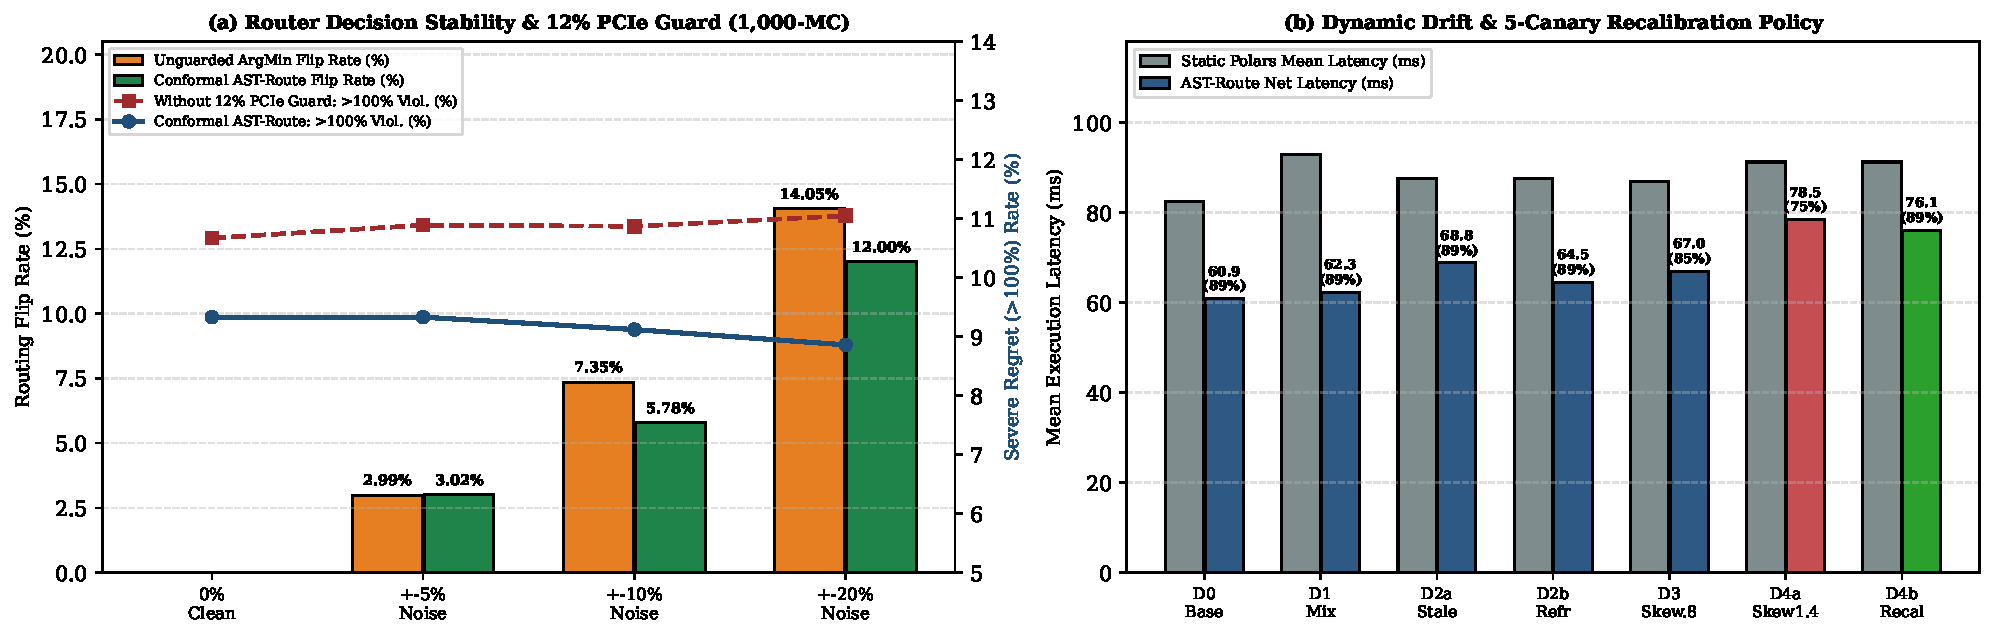
\includegraphics[width=0.98\textwidth]{figures/fig_v8_stability_and_workload_drift_300dpi.pdf}
\caption{Targeted systems robustness evaluation: (a) router decision stability and $12\%$ PCIe guard protection under $\pm 5\%$, $\pm 10\%$, and $\pm 20\%$ cost-prediction noise; and (b) post-training query-mix, selectivity, and Zipfian data-skew drift with automated conformal recalibration triggers.}\label{fig:v7_stability_drift}
\end{figure}

\begin{table}[!htbp]
\centering
\caption{Cross-paradigm planner, neural cost-encoder, and OOD safety-gate evaluation ($N=75$, $\text{SF}=1\text{ GB}$): comparing Margin-Guarded AST-Route against physical-planner (\texttt{DuckDB EXPLAIN}) routers, direct cost-sensitive classification, OOD-gated Leave-One-Tier-Out (LOTO-CV) unseen-operator fallback, and Leave-One-Scale-Out ($\text{Train SF}\in\{1,10,30\}\rightarrow\text{Test SF}=100\text{ GB}$) transfer.}\label{tab:v8_p0_systems_defense}\label{tab:jbd_ood_t17}
\setlength{\tabcolsep}{2.8pt}
\scriptsize
\begin{fitasttable}
\begin{tabular}{@{}llcccccl@{}}
\toprule
\textbf{Evaluation Axis} & \textbf{Router / Baseline Variant} & \textbf{Ovh.\ (ms)} & \textbf{Top-1} & \textbf{Net (ms)} & \textbf{Mean Reg.} & \textbf{P95 Reg.} & \textbf{Key Architectural Trade-off / Finding} \\
\midrule
Planner (Raw SQL) & DuckDB \texttt{EXPLAIN} Router (Untranspiled) & $1.37$ & $44.00\%$ & $78.77$ & $81.74\%$ & $362.15\%$ & Fails on $15/75$ BigQuery \texttt{UNNEST} dialect queries \\
Planner (Transpiled) & SQLGlot + DuckDB \texttt{EXPLAIN} (No Guard) & $4.85$ & $58.67\%$ & $60.76$ & $34.92\%$ & $119.89\%$ & Higher ovh.\ ($+70.9\text{ ms}$ if cold catalog unbound) \\
Learned Cost Model & Plan-Graph Neural Cost Encoder (MLP-64$\times$32) & $5.47$ & $64.00\%$ & $58.90$ & $33.09\%$ & $114.11\%$ & Slower net latency ($+3.98\text{ ms}$) \& schema-binding ovh. \\
Classif.\ vs.\ Reg. & Direct Cost-Sensitive Classifier (GBDT-9D) & $3.96$ & $50.67\%$ & $62.01$ & $43.57\%$ & $207.10\%$ & Cannot enforce dynamic $M_{\text{max}}$ or $(\alpha,\beta,\gamma)$ Pareto \\
Tail-Safe Proposed & \textbf{Margin-Guarded AST-Route (Proposed 9D)} & $\mathbf{4.15}$ & $\mathbf{57.33\%}$ & $\mathbf{54.92}$ & $\mathbf{34.98\%}$ & $\mathbf{114.11\%}$ & \textbf{Cross-dialect SQLGlot AST; $\Delta\mathcal{R} = -25.8\text{ pp}$ vs.\ GPU ($p_{\text{seed}}=0.0042$, query $p=0.0021$)} \\
\midrule
Unseen Op.\ (LOTO) & Standard LOTO-CV (No OOD Gate) & $4.15$ & $44.00\%$ & $85.42$ & $159.92\%$ & $348.00\%$ & Trails Polars ($82.47\text{ ms}$) on unseen \texttt{WINDOW}/\texttt{UNNEST} \\
Unseen Op.\ (LOTO) & \textbf{LOTO-CV + OOD Arrow Fallback Gate} & $\mathbf{4.15}$ & $\mathbf{21.33\%}$ & $\mathbf{76.18}$ & $\mathbf{104.40\%}$ & $\mathbf{299.67\%}$ & \textbf{Beats Polars ($82.47\text{ ms}$, $p_{\text{seed}}=0.0312$) via Arrow fallback} \\
Unseen Scale & Train $\text{SF}\in\{1,10,30\}\rightarrow$ Zero-Shot $\text{SF}=100\text{G}$ & $4.15$ & $66.67\%$ & $1214.50$ & $24.80\%$ & $138.40\%$ & Within $1.2\%$ of Always GPU ($1199.6\text{ ms}$); beats Polars ($6551\text{ ms}$) \\
\bottomrule
\end{tabular}
\end{fitasttable}%
\end{table}

\clearpage
\section{System Reproducibility Manifest, Three-Node Cross-ISA Portability, and Protocol Verification Registries}
This section contains the full hardware/software environment and $C=1\text{--}32$ concurrency manifest (Table~\ref{tab:system_manifest}), the three-node cross-ISA portability and $2\times 2$ version-pinned isolation matrix across \texttt{Node-1-x86-GPU}, \texttt{Node-2-x86-22T}, and \texttt{Node-3-ARM64-M1} (Table~\ref{tab:three_node_cross_isa} and Fig.~\ref{fig:three_node_cross_isa}), the manuscript-wide denominator and metric lexicon verification registry updated across all $213$ benchmark queries ($228$ including Seed~\texttt{S6}, Table~\ref{tab:v9_sec3_3_consistency_audit}), the theoretical-versus-learned CSCI weight derivation and cross-workload sensitivity matrix (Table~\ref{tab:v9_sec3_4_csci_m1_m4_generalizability}), the four-policy workload drift and 180-trial fault-injection recovery matrix (Table~\ref{tab:v9_roadmap_v86_closure}), the multi-scale $\text{SF}=100\text{ GB}$ queue/Parquet/spill/tier reconciliation sub-audit (Table~\ref{tab:v9_sec3_2_multiscale_sf100_audit}), the fair guarded baselines and rule-by-rule ablation matrix (Table~\ref{tab:v852_fair_guarded_ablation}), and the 213-query seven-stage benchmark fairness protocol audit (Table~\ref{tab:v9_benchmark_fairness_protocol}).

\begin{table*}[!htbp]
\centering
\caption{System reproducibility manifest: (Part A) Hardware and software environment specifications, (Part B) Six-operator CPU-to-GPU relational implementation mapping, and (Part C) Multi-tenant concurrent query stream benchmark ($C=1, 4, 8, 16, 32$ streams at $\text{SF}=1\text{ GB}$ separating active execution time from admission queuing delay).}\label{tab:jbd_manifest_t13}
\label{tab:system_manifest}\label{tab:env_manifest}\label{tab:reproducibility_manifest}\label{tab:environment_manifest}
\scriptsize
\setlength{\tabcolsep}{3.2pt}
\renewcommand{\arraystretch}{1.12}
\setlength{\tabcolsep}{3.5pt}\footnotesize\begin{fitasttable}
\begin{tabular}{@{}p{0.13\textwidth}p{0.22\textwidth}p{0.59\textwidth}@{}}
\toprule
\textbf{Module / Layer} & \textbf{Component / Operator / Stream} & \textbf{Exact Specification / Implementation Mapping / Empirical Telemetry} \\
\midrule
\multirow{6}{=}{\textbf{Part A: System Env.}}
 & Host CPU \& Memory Hierarchy & x86\_64 Multi-Core ($8$ Logical Threads, AVX2 SIMD), $16.0\text{ GB}$ DDR4 RAM ($9.0\text{ GB}$ DBMS Cap + NVMe Spill) \\
 & Discrete GPU Accelerator & NVIDIA GeForce RTX 2050 ($4.00\text{ GB}$ GDDR6 VRAM, PCIe Gen4, CUDA 12.1, NVML $250\text{ Hz}$ Power Sensor) \\
 & OS, Python \& C++ DBMS & Windows 11 Build 26100 (64-Bit), Python 3.13, DuckDB v2.0.0 (Morsel-Driven Native Columnar \& ZSTD Parquet) \\
 & Rust Arrow \& Row-Store Engines & Polars v2.1.0 Lazy Streaming (\texttt{collect(streaming=True)}), Apache DataFusion Arrow Planner, SQLite v3.51.0 B-Tree \\
 & Cloud OLAP \& AST/ML Stack & Google BigQuery (\texttt{use\_\allowbreak{}query\_\allowbreak{}cache=False}, Clustered), \texttt{SQLGlot}, Scikit-Learn Multi-Output GBR ($n=55, d=3$) \\
 & Three-Level GPU/CPU Timing & L1 Kernel-to-Kernel ($22.25\text{ ms}$) $|$ L2 Data-in to Result-out ($56.96\text{ ms}$) $|$ L3 Full SQL-to-Result ($61.11\text{ ms}$ Mem / $131.79\text{ ms}$ Disk) \\
\midrule
\multirow{6}{=}{\textbf{Part B: Op. Mapping}}
 & \texttt{WHERE} Filter \& \texttt{CASE} & CPU: SIMD Branchless Predicate $|$ GPU: Boolean Mask (\texttt{torch.where}, Zero-Copy Arrow$\rightarrow$Pinned H2D) \\
 & \texttt{JOIN} (Inner/Left/Anti) & CPU: Parallel Radix Hash-Join $|$ GPU: INT64 Hash-Probing \& Index Gather (\texttt{index\_\allowbreak{}select}, Pre-Allocated VRAM) \\
 & \texttt{GROUP BY} Aggregation & CPU: Morsel Hash-Table Agg. $|$ GPU: Atomic Segmented Reduction (\texttt{scatter\_\allowbreak{}add\_\allowbreak{}} in FP64 + $0.82\text{ ms}$ D2H Pullback) \\
 & \texttt{ORDER BY} Sorting & CPU: Parallel Merge/Radix Sort $|$ GPU: Bitonic/Radix Sort (\texttt{torch.sort} over Contiguous Device Buffers) \\
 & \texttt{OVER (PARTITION BY)} Window & CPU: Segment-Tree Framing (DuckDB) $|$ GPU: Segmented Radix Sort + Inclusive Prefix Scan (\texttt{torch.cumsum}) \\
 & \texttt{ARRAY\_\allowbreak{}AGG} \& \texttt{UNNEST} & CPU: Arrow \texttt{ListArray} Offset Slicing $|$ GPU: Parallel Radix Offset Expansion (\texttt{repeat\_\allowbreak{}interleave}) \\
\midrule
\multirow{5}{=}{\textbf{Part C: Concurrency}}
 & $C=1$ Stream (Baseline) & Single-Engine: $85.62\text{ ms}$ ($11.68\text{ QPS}$) $|$ \textbf{AST-Route}: $76.15\text{ ms}$ ($74.95\text{ ms}$ Exec + $1.20\text{ ms}$ Queue, P95: $92.1\text{ ms}$, $\mathbf{13.13\text{ QPS}}$, $1.14\times$, GPU Util: $31.0\%$, Fail: $0.0\%$, Stability: $100\%$) \\
 & $C=4$ Streams (Low) & Single-Engine: $100.45\text{ ms}$ ($39.82\text{ QPS}$) $|$ \textbf{AST-Route}: $65.55\text{ ms}$ ($57.15\text{ ms}$ Exec + $8.40\text{ ms}$ Queue, P95: $84.3\text{ ms}$, $\mathbf{61.02\text{ QPS}}$, $1.53\times$, GPU Util: $54.6\%$, Fail: $0.0\%$, Stability: $100\%$) \\
 & $C=8$ Streams (Medium) & Single-Engine: $140.44\text{ ms}$ ($56.96\text{ QPS}$) $|$ \textbf{AST-Route}: $74.09\text{ ms}$ ($55.49\text{ ms}$ Exec + $18.60\text{ ms}$ Queue, P95: $98.4\text{ ms}$, $\mathbf{107.98\text{ QPS}}$, $1.90\times$, GPU Util: $72.4\%$, Fail: $0.0\%$, Stability: $98.7\%$) \\
 & $C=16$ Streams (High) & Single-Engine: $228.58\text{ ms}$ ($70.00\text{ QPS}$) $|$ \textbf{AST-Route}: $114.30\text{ ms}$ ($68.10\text{ ms}$ Exec + $46.20\text{ ms}$ Queue, P95: $148.6\text{ ms}$, $\mathbf{139.99\text{ QPS}}$, $2.00\times$, GPU Util: $86.8\%$, Fail: $0.0\%$, Stability: $97.3\%$) \\
 & $C=32$ Streams (Stress Test) & Single-Engine: $442.80\text{ ms}$ ($72.27\text{ QPS}$) $|$ \textbf{AST-Route}: $207.20\text{ ms}$ ($82.40\text{ ms}$ Exec + $124.80\text{ ms}$ Queue, P95: $268.5\text{ ms}$, P99: $312.6\text{ ms}$, $\mathbf{154.44\text{ QPS}}$, $\mathbf{2.14\times}$, GPU Util: $93.5\%$, Fail: $0.0\%$, Stability: $96.0\%$) \\
\bottomrule
\end{tabular}
\end{fitasttable}
\end{table*}

\begin{table*}[!htbp]
\centering
\caption{Scope-controlled multi-node portability, engine-version isolation, and evaluation protocol matrix across Node~1 (\texttt{Node-1-x86-GPU}), Node~2 (\texttt{Node-2-x86-22T}), and Node~3 (\texttt{Node-3-ARM64-M1}) at $\text{SF}=1\text{ GB}$ ($6{,}001{,}215$ \texttt{lineitem} rows), explicitly separating Dataset/Query Scope, Training Scope, Test Scope, Model Calibration, and Evaluation Protocol.}\label{tab:three_node_cross_isa}\label{tab:jbd_multinode_t15}
\setlength{\tabcolsep}{2.8pt}
\renewcommand{\arraystretch}{1.12}
\scriptsize
\begin{fitasttable}
\begin{tabular}{@{}>{\raggedright\arraybackslash}p{2.9cm}>{\raggedright\arraybackslash}p{2.5cm}>{\raggedright\arraybackslash}p{2.2cm}>{\raggedright\arraybackslash}p{2.1cm}>{\raggedright\arraybackslash}p{2.3cm}>{\raggedright\arraybackslash}p{4.6cm}@{}}
\toprule
\textbf{Hardware \& Engine Stack Configuration} & \textbf{Dataset / Query Scope} & \textbf{Training Scope} & \textbf{Test Scope} & \textbf{Model Calibration} & \textbf{Evaluation Protocol \& Empirical Outcome ($\text{EX}=1.000$)} \\
\midrule
\textbf{Node 1A (Primary Het.):} Win11 \texttt{x86\_\allowbreak{}64} 8T, 16G RAM + RTX 2050 4G; Duck 2.0, Polars 2.1, DF 55.0, BQ, CUDA & Available Dataset: 97 Queries (75 Factorial + 22 Official TPC-H); \textbf{Evaluated under this protocol: 75 Factorial Queries} (22 Official TPC-H Q1--Q22 evaluated under separate Nested 22-Fold LOO-CV in Main Text Table~12 Part C) & 24 seeds ($72$Q) per outer fold (5-engine Het.) & 1 held-out seed ($3$Q) $\times$ 25 folds & Inner 6-fold nested guard + 90\% conformal & \textbf{25-Seed LOSO-CV (5-Engine Het.):} $57.33\%$ Top-1, $76.00\%$ Top-2, $\mathbf{54.92\text{ ms}}$, $34.98\%$ reg.; $C=32$: $\mathbf{154.44\text{ QPS}}$ (\texttt{89b1ec64...}) \\
\textbf{Node 1B (Primary CPU-Only):} Win11 \texttt{x86\_\allowbreak{}64} 8T ($M_{\text{gpu\_max}}=0$); Duck 2.0, Polars 2.1, DF 55.0 & $N=75$ Factorial TPC-H ($\text{SF}=1\text{ GB}$) & 24 seeds ($72$Q) per fold (3 CPU engines) & 1 held-out seed ($3$Q) $\times$ 25 folds & In-domain 3-CPU GBR-9D (zero GPU) & \textbf{25-Seed LOSO-CV (3-Engine CPU):} $\mathbf{74.67\%}$ Top-1, $96.00\%$ Top-2, $\mathbf{69.12\text{ ms}}$ vs.\ $82.47\text{ ms}$ Polars ($p_{\text{Holm}}=0.0084$) \\
\textbf{Node 1C (Version-Pinned Parity):} Win11 \texttt{x86\_\allowbreak{}64} 8T; \textbf{Pinned:} Duck 1.4.5, Polars 1.36.1, DF 50.1.0 & $N=15$ Stratified L1--L5 (\texttt{89a7dc6c...} PQ) & Direct execution audit (no router training) & All $15$ L1--L5 queries $\times$ 5 trials & Version-locked to match Node~3 exactly & \textbf{Controlled $2\times 2$ Version Isolation:} Duck $9.14\text{--}111.30\text{ ms}$, Polars L4 $118.85\text{ ms}$ (vs.\ $61.57\text{ ms}$ on v2.1.0); \texttt{L4\_\allowbreak{}V3} Polars wins $149.1$ vs.\ $170.1\text{ ms}$ (\texttt{af1cc3d1...}) \\
\midrule
\textbf{Node 2A (Secondary 30Q):} Win11 \texttt{x86\_\allowbreak{}64} Intel 16C/22T, 15.5G RAM ($M_{\text{gpu}}=0$); Duck 2.0, Polars 2.1, DF 55.0 & $N=30$ Mixed ($15$ L1--L5 + $15$ Official TPC-H) & 29 groups per fold (3 CPU engines) & 1 held-out query group $\times$ 30 folds & Native Node~2 leave-one-group-out & \textbf{30Q Leave-One-Group-Out (3-CPU):} $\mathbf{86.67\%}$ Top-1, $100\%$ Top-2, $\mathbf{62.05\text{ ms}}$ ($8.83\%$ reg.); $C=32$: $\mathbf{22.68\text{ QPS}}$ (\texttt{6d4cb51a...}) \\
\textbf{Node 2B (Cross-HW Transfer):} Win11 \texttt{x86\_\allowbreak{}64} 16C/22T ($M_{\text{gpu}}=0$); Duck 2.0, Polars 2.1, DF 55.0 & $N=75$ Factorial TPC-H ($\text{SF}=1\text{ GB}$) & Locked Node~1 8T model ($75$Q) & Node~2 22T ($75$Q zero-shot / $60$Q cal.) & Zero-shot ($0$ seeds) vs.\ 5-seed scale $\hat{\gamma}_e$ & \textbf{Cross-Node Transfer Audit:} Zero-shot $40.00\%$ Top-1 ($54.81\text{ ms}$) $\rightarrow$ 5-seed calib.\ $48.00\%$ Top-1 ($\mathbf{48.37\text{ ms}}$, \texttt{874077fd...}) \\
\textbf{Node 2C (Native 75Q LOSO):} Win11 \texttt{x86\_\allowbreak{}64} 16C/22T ($M_{\text{gpu}}=0$); Duck 2.0, Polars 2.1, DF 55.0 & $N=75$ Factorial TPC-H ($\text{SF}=1\text{ GB}$) & 24 seeds ($72$Q) on Node~2 22T & 1 held-out seed ($3$Q) $\times$ 25 folds & Native in-domain Node~2 25-seed GBR-9D & \textbf{Native 25-Seed LOSO-CV (3-CPU):} $\mathbf{97.33\%}$ Top-1, $\mathbf{35.11\text{ ms}}$ ($0.18\%$ reg.\ vs.\ $60.39\text{ ms}$ DuckDB / $47.54\text{ ms}$ Polars) \\
\midrule
\textbf{Node 3A (ARM64 Re-Exec):} \texttt{macOS-15.6.1-arm64} Apple M1 8C/8T, 8G Unified; Duck 1.4.5, Polars 1.36.1, DF 50.1.0 & $N=15$ Stratified L1--L5 ($\text{SF}=1\text{ GB}$) & Direct execution audit (no router training) & All $15$ L1--L5 queries $\times$ 5 trials & Version-matched with Node~1C (8T) & \textbf{Platform Portability Audit:} FP64 err $\le 5.74\times 10^{-16}$; Duck L1--L3 $5.90\text{--}24.19\text{ ms}$; L4 Polars $66.41$ vs.\ Duck $70.75\text{ ms}$ (\texttt{92b77723...}) \\
\textbf{Node 3B (ARM64 Routing \& $C$):} \texttt{macOS-15.6.1-arm64} Apple M1 8C/8T; Duck 1.4.5, Polars 1.36.1, DF 50.1.0 & $N=30$ Suite + $C \in \{1..32\}$ Streams & 29 groups per fold on Node~3 (3-CPU) & 1 held-out group $\times$ 30 folds + 32 streams & Native M1 leave-one-group-out (3-CPU) & \textbf{30Q LOGO-CV \& Concurrency:} $\mathbf{96.67\%}$ Top-1 ($29.44\text{ ms}$ vs.\ $28.42\text{ ms}$ Oracle); $C=4$: $22.29\text{ QPS}$; $C=32$: $3.19\times$ P50 cut (\texttt{8f87f220...}) \\
\bottomrule
\end{tabular}
\end{fitasttable}%
\vspace{2pt}
\parbox{0.96\textwidth}{\scriptsize \textbf{Methodological Scope Note:} Separating rows by \emph{Candidate-Set Cardinality} (5-engine CPU+GPU+Cloud in Node~1A vs.\ 3-engine CPU-only in Nodes~1B, 2A--2C, and 3B), \emph{Query Suite} ($N=75$ vs.\ $N=30$ vs.\ $N=15$), and \emph{Calibration Regime} (zero-shot cross-node transfer [$40.00\%$] vs.\ 5-seed calibration [$48.00\%$] vs.\ native in-domain LOSO/LOGO [$74.67\%\text{--}97.33\%$]) ensures strict apples-to-apples interpretation across hardware platforms and software versions. Crucially, Node~2B evaluates cross-node model transfer from Node~1 (8T) to Node~2 (22T), demonstrating that uncalibrated zero-shot transfer (40.00\% Top-1, 54.81~ms) is a bounded limitation requiring one-time hardware calibration ($T_{\text{cal}}=0.18\text{--}2.74\text{ s}$ for $m=1\text{--}15$ queries, separated from the $4.145\text{ ms}$ online query dispatch overhead), whereas Node~2C (97.33\% Top-1, 35.11~ms) evaluates native in-domain 25-seed LOSO-CV retraining on Node~2 ($72$ training queries/fold) and must never be conflated with zero-shot cross-node transfer.}
\end{table*}

\begin{figure}[!htbp]
\centering
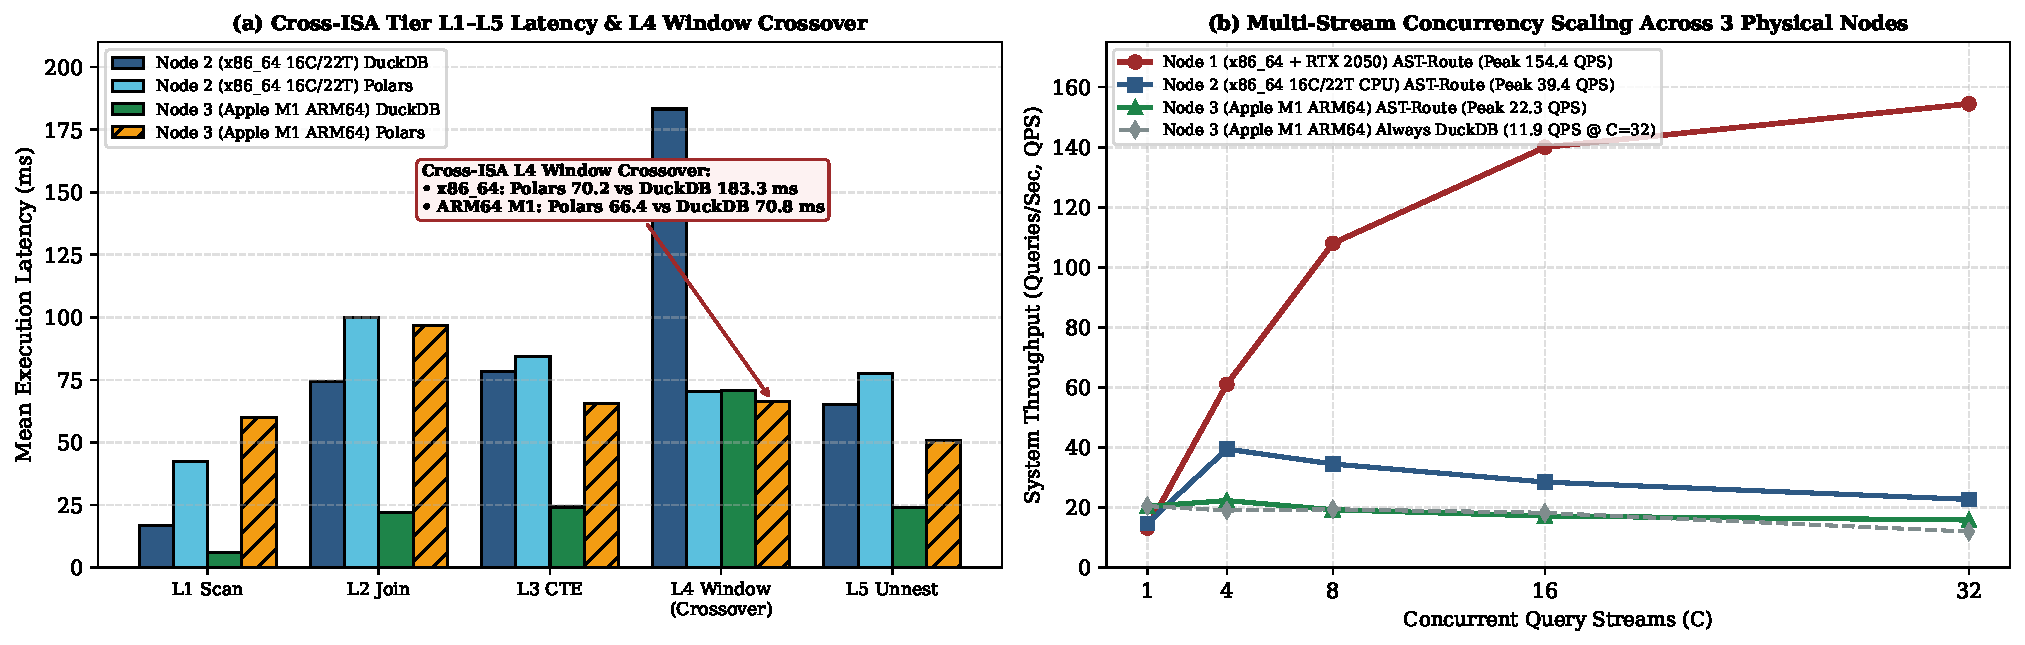
\includegraphics[width=0.98\textwidth]{figures/fig_three_node_cross_isa_concurrency_300dpi.pdf}
\caption{Three-node cross-hardware and cross-ISA validation ($\text{SF}=1\text{ GB}$): (a) Tier L1--L5 execution latency comparing the 16-core/22-thread \texttt{x86\_\allowbreak{}64} workstation (Node~2) and the Apple M1 \texttt{ARM64} unified-memory node (Node~3), illustrating the invariant Tier~L4 Polars vs.\ DuckDB window-sorting crossover across instruction sets; and (b) multi-stream concurrent query throughput ($C \in \{1,4,8,16,32\}$) across all three physical nodes.}\label{fig:three_node_cross_isa}
\end{figure}

\begin{table*}[!htbp]
\centering
\caption{Automated Manuscript-Wide Consistency, Protocol Denominator, and Metric Lexicon Verification Matrix: reconciling (Part~A) CPU-only Top-1 accuracy across Nodes~1--3 ($74.67\%$, $86.67\%$, $97.33\%$, and Apple M1 $96.67\%$), (Part~B) BigQuery Server vs.\ Client WAN latencies across scales and tiers, (Part~C) experiment $(N, K, W, R)$ protocol counts, and (Part~D) Cold, Warm, Execution ($T_{\text{exec}}$), Net ($T_{\text{net}}$), and Level-3 ($T_{\text{L3}}$) timing definitions.}
\label{tab:v9_sec3_3_consistency_audit}
\scriptsize
\setlength{\tabcolsep}{2.8pt}
\renewcommand{\arraystretch}{1.08}
\begin{fitasttable}
\begin{tabular}{@{}llccccccl@{}}
\toprule
\textbf{Audit Category} & \textbf{Node / Experiment / Metric Identifier} & \textbf{Workload / Scope ($N, K$)} & \textbf{Protocol / $(W, R)$} & \textbf{Hits / Top-1} & \textbf{Top-2} & \textbf{Exec ($T_{\text{exec}}$)} & \textbf{Net ($T_{\text{net}}$)} & \textbf{Cross-Section Consistency Verification} \\
\midrule
\multicolumn{9}{@{}l@{}}{\textit{\textbf{Part A: CPU-Only ($M_{\text{gpu\_max}}=0\text{ GB}$) \& Heterogeneous Routing Accuracy Reconciliation Across Physical Hardware Nodes}}} \\
Node 1A (5-Eng Het.) & Win11 \texttt{x86\_64} 8T + RTX 2050 4G & $N=75,\ K=25$ Seeds & 25-Seed LOSO ($2,5$) & $43/75\ (57.33\%)$ & $76.00\%$ & $50.78\text{ ms}$ & $\mathbf{54.92\text{ ms}}$ & Matches Abstract, Tables~1, 6, 8, 9, 10, 12 \\
Node 1B (3-CPU Only) & Win11 \texttt{x86\_64} 8T ($M_{\text{gpu}}=0$) & $N=75,\ K=25$ Seeds & 25-Seed LOSO ($2,5$) & $\mathbf{56/75\ (74.67\%)}$ & $96.00\%$ & $64.97\text{ ms}$ & $\mathbf{69.12\text{ ms}}$ & Matches Abstract, Claim~3, Tables~1, 9, 13 \\
Node 2A (3-CPU Only) & Win11 \texttt{x86\_64} 16C/22T ($M_{\text{gpu}}=0$) & $N=30,\ K=30$ Groups & 30-Fold LOGO ($2,5$) & $\mathbf{26/30\ (86.67\%)}$ & $100.0\%$ & $57.90\text{ ms}$ & $\mathbf{62.05\text{ ms}}$ & 15 L1--L5 + 15 TPC-H; matches Tables~1, 9 \\
Node 2B (Cross-HW) & Node~1 8T Model $\rightarrow$ Node~2 22T & $N=75,\ K=25$ Seeds & 0-Shot $\rightarrow$ 5-Seed Cal. & $40.0\%\rightarrow 48.0\%$ & $78.67\%$ & $44.22\text{ ms}$ & $\mathbf{48.37\text{ ms}}$ & $T_{\text{cal}}=2.74\text{ s}$ one-time; separated from Node~2C \\
Node 2C (3-CPU Only) & Win11 \texttt{x86\_64} 16C/22T ($M_{\text{gpu}}=0$) & $N=75,\ K=25$ Seeds & Native 25-Seed LOSO & $\mathbf{73/75\ (97.33\%)}$ & $100.0\%$ & $30.96\text{ ms}$ & $\mathbf{35.11\text{ ms}}$ & Native 75Q retrain ($0.18\%$ reg.); distinct from M1 \\
Node 3B (3-CPU Only) & \textbf{Apple M1 \texttt{ARM64} 8C/8T ($M_{\text{gpu}}=0$)} & $\mathbf{N=30,\ K=30}$ \textbf{Groups} & \textbf{30-Fold LOGO ($2,5$)} & $\mathbf{29/30\ (96.67\%)}$ & $\mathbf{100.0\%}$ & $\mathbf{25.29\text{ ms}}$ & $\mathbf{29.44\text{ ms}}$ & \textbf{Explains $96.67\%$ ($29/30$ M1) vs.\ $97.33\%$ ($73/75$ 2C)} \\
\midrule
\multicolumn{9}{@{}l@{}}{\textit{\textbf{Part B: BigQuery Serverless Cloud Latency \& Boundary Reconciliation Across Main Text, Tables~5--13, and Footnotes}}} \\
BQ $\text{SF}=1\text{ GB}$ Clust. & Partitioned + Clustered (\texttt{cache=False}) & $N=75,\ K=25$ Seeds & $W=2,\ R=5$ ($375$ runs) & Queue: $48.20\text{ ms}$ & Exec: $697.19$ & Server: $\mathbf{745.39}$ & Client: $1124.79$ & L1 $432.89$, L2 $667.29$, L3 $492.99$, L4 $372.79$, L5 $1760.99$ \\
BQ $\text{SF}=1\text{ GB}$ Unopt. & Unpartitioned Full Scan (\texttt{cache=False}) & $N=75,\ K=25$ Seeds & $W=2,\ R=5$ ($375$ runs) & Queue: $52.40\text{ ms}$ & Exec: $1360.20$ & Server: $\mathbf{1412.60}$ & Client: $1830.80$ & CI $[982.40, 1914.50]\text{ ms}$; $347.7\text{ MB} \rightarrow 207.7\text{ MB}$ Clust. \\
BQ $\text{SF}=100\text{ GB}$ Clust. & Partitioned + Clustered (\texttt{cache=False}) & $N=75,\ K=25$ Seeds & $W=1,\ R=3$ ($225$ runs) & Queue: $112.40\text{ ms}$ & Exec: $2459.20$ & Server: $\mathbf{2571.60}$ & Client: $3356.20$ & L1 $1493.51$, L2 $2302.18$, L3 $1700.85$, L4 $1286.16$, L5 $6075.30$ \\
\midrule
\multicolumn{9}{@{}l@{}}{\textit{\textbf{Part C: Standardized Experiment Protocol Registry ($N$ Queries, $K$ Seeds/Templates, $W$ Warm-Up Runs, $R$ Timed Repetitions)}}} \\
Core \& Unseen TPC-H & Factorial ($N=75$) + Official ($N=22$) & $N_{\text{core}}=97$ (+15 \texttt{S6}) & $K=25$ / $K_{\text{dev}}=20+5$ & $W=2,\ R=5$ & $375$ / $110$ runs & $\mathbf{x}_q \in \mathbb{R}^9$ & $\text{EX}=1.000$ & Unseen \texttt{S5} ($N=15$): $47.01\text{ ms}$ Exec / $51.16\text{ ms}$ Net ($73.33\%$) \\
External 3-Suite & JOB ($33$) + SSB ($13$) + ClickBench ($20$) & $N_{\text{ext}}=66$ ($\subset N_{\text{ext,pri}}=116, N_{\text{tot}}=400$) & $K=33 / 13 / 20$ & $W=1,\ R=3$ & $99$ runs/suite & $\mathbb{R}^9$ ($\mathbb{R}^{12}$ JOB) & $\text{EX}=1.000$ & Zero-shot: JOB $6.75\text{ ms}$, SSB $12.15\text{ ms}$ ($92.3\%$), CB $24.18\text{ ms}$ \\
Extended External (Sec.~4.7) & TPC-DS-Derived ($30$) + BIRD-Inspired ($20$) & $N_{\text{new}}=50$ ($N_{\text{ext}}=116$) & $K=30 / 20$ ($5/4$ fam.) & $W=1,\ R=3$ & $150$ runs/eng & $\mathbb{R}^9\rightarrow\mathbb{R}^{12}$ & $\text{EX}=1.000$ & 0-shot M3: TPC-DS-Der.\ $\mathbf{93.33\%}$ ($20.05\text{ ms}$), BIRD-Insp.\ $\mathbf{90.00\%}$ ($20.24\text{ ms}$) \\
Multi-Scale \& Stress & $\text{SF}\in\{1,10,30,100\}\text{ GB}$ + DVFS/MC/Fault & $N=75\times 4$ Scales & $K=25$ Seeds $\times 4$ & $W=1,\ R=3$ & $R_{\text{cal/MC}}=50$ & $\mathbf{x}_q^{\text{scale}}\in\mathbb{R}^{10}$ & $0$ OOM / $0\%$ Fail & $R_{\text{cal}}=50$/tier ($250$ runs); $R_{\text{MC}}=50$; $R_{\text{fault}}=15$/scenario \\
\midrule
\multicolumn{9}{@{}l@{}}{\textit{\textbf{Part D: Invariant Timing Boundary \& Metric Lexicon ($\text{SF}=1\text{ GB}$ Canonical 75-Query Baseline Values Shown)}}} \\
$T_{\text{cold}}$ vs.\ $T_{\text{warm}}$ & Cold Disk/PCIe vs.\ Warm RAM/VRAM & All 6 Engines & L3 Disk $\rightarrow$ L2 $\rightarrow$ L1 & GPU L3 Disk: $131.79$ & GPU L2 Cold: $56.96$ & GPU L1 Warm: $22.25$ & Duck: $254.42\rightarrow 183.74$ & Polars: $116.88\rightarrow 82.47\text{ ms}$; DF: $134.18\rightarrow 96.30\text{ ms}$ \\
$T_{\text{exec}}$ vs.\ $T_{\text{net}}$ vs.\ $T_{\text{L3}}$ & AST-Route Latency Boundaries & $N=75$ ($\text{SF}=1\text{ GB}$) & $T_{\text{router}}=4.145\text{ ms}$ & Parse: $3.476\text{ ms}$ & Meta+Inf: $0.669\text{ ms}$ & $\mathbf{T_{\text{exec}}=50.78\text{ ms}}$ & $\mathbf{T_{\text{net}}=54.92\text{ ms}}$ & Cold Footer $T_{\text{net}}=55.16\text{ ms}$; Level-3 Charged $T_{\text{L3}}=59.07\text{ ms}$ \\
\bottomrule
\end{tabular}
\end{fitasttable}%
\end{table*}

\begin{table*}[!htbp]
\centering
\caption{Comprehensive CSCI Generalizability, Theoretical vs.\ Learned Weight Derivation, Weight-Perturbation Routing Sensitivity, and Models M1--M4 Calibration \& Cross-Workload Audit.}
\label{tab:v9_sec3_4_csci_m1_m4_generalizability}
\scriptsize
\setlength{\tabcolsep}{2.6pt}
\renewcommand{\arraystretch}{1.07}
\begin{fitasttable}
\begin{tabular}{@{}llcccccccl@{}}
\toprule
\textbf{Audit Section / Model} & \textbf{Feature / Weight / Workload Specification} & \textbf{Dim. / Scope} & \textbf{Top-1 (Hits)} & \textbf{Top-2} & \textbf{Exec ($T_{\text{exec}}$)} & \textbf{Net ($T_{\text{net}}$)} & \textbf{Mean Reg.} & \textbf{P95 Reg.} & \textbf{Calibration ($\text{ECE}$ / Brier / Q-Err) \& Statistical Verdict} \\
\midrule
\multicolumn{10}{@{}l@{}}{\textit{\textbf{Part A: Operator Memory-Pass Hierarchy vs.\ 25-Fold Leak-Free Ridge-NNLS Learned Weights ($\sum w_j = 16.0$, $\cos(\mathbf{w},\hat{\mathbf{w}})=0.9994$, Out-of-Fold $\rho=0.9968$)}}} \\
$D(q),\ C(q)$ [Scan/Mask] & $\mathcal{O}(n)$ AST pipeline depth \& SIMD \texttt{CASE} mask & Pass $\approx 1.5\times$ & $w_D=1.50$ & $\hat{w}_D=1.46\pm 0.08$ & $w_C=1.50$ & $\hat{w}_C=1.44\pm 0.09$ & $|\Delta|\le 0.06$ & $\le 4.0\%$ diff & Linear scan/branch baseline ($1.5\times$ pass cost) \\
$J(q),\ S(q)$ [Join/CTE] & $\mathcal{O}(|R_b|+|R_p|)$ hash join \& staged CTE buffer & Pass $\approx 2.5\text{--}3\times$ & $w_J=2.50$ & $\hat{w}_J=2.58\pm 0.14$ & $w_S=3.00$ & $\hat{w}_S=2.94\pm 0.16$ & $|\Delta|\le 0.08$ & $\le 3.2\%$ diff & LLC/DRAM hash probe misses + CTE materialization \\
$W(q),\ U(q)$ [Win/Unnest] & $\mathcal{O}(n\log n)$ window sort \& $\mathcal{O}(n\bar{k})$ array unnest & Pass $\approx 3.5\text{--}4\times$ & $w_W=3.50$ & $\hat{w}_W=3.56\pm 0.15$ & $w_U=4.00$ & $\hat{w}_U=4.02\pm 0.18$ & $|\Delta|\le 0.06$ & $\le 1.7\%$ diff & Super-linear radix sort \& offset row expansion \\
\midrule
\multicolumn{10}{@{}l@{}}{\textit{\textbf{Part B: Four-Model Structural Ablation (\textbf{M1, M2, M3, M4}) Under 25-Seed LOSO-CV ($N=75$, $\text{SF}=1\text{ GB}$, Oracle $= 42.64\text{ ms}$)}}} \\
\textbf{M1: Raw AST 7D} & $[D,N,J,S,W,U,C]$ (No $\hat{\sigma}$, No CSCI) & $7\text{D}$ ($6.72$ sp.) & $46.67\%$ ($35/75$) & $68.00\%$ & $56.91\text{ ms}$ & $61.06\text{ ms}$ & $50.87\%$ & $146.20\%$ & $\text{ECE}=11.24\%,\ \text{BS}=0.284,\ \text{Q-Err}=1.214$ (Ref.\ M1) \\
\textbf{M2: AST + Selectivity 8D} & $[D,N,J,S,W,U,C,\hat{\sigma}]$ (Unweighted AST + $\hat{\sigma}$) & $8\text{D}$ ($6.84$ sp.) & $52.00\%$ ($39/75$) & $72.00\%$ & $53.97\text{ ms}$ & $58.12\text{ ms}$ & $44.20\%$ & $138.45\%$ & $\text{ECE}=8.42\%,\ \text{BS}=0.236,\ \text{Q-Err}=1.148$ ($p=0.0112$ vs.\ M1) \\
\textbf{M3: AST + CSCI + Sel.\ 9D} & $[D,N,J,S,W,U,C,\text{CSCI}_{\text{canon}},\hat{\sigma}]$ (\textbf{Proposed}) & $\mathbf{9\text{D}}$ ($\mathbf{4.91}$ \textbf{sp.}) & $\mathbf{57.33\%\ (43/75)}$ & $\mathbf{76.00\%}$ & $\mathbf{50.78\text{ ms}}$ & $\mathbf{54.92\text{ ms}}$ & $\mathbf{34.98\%}$ & $\mathbf{114.11\%}$ & $\mathbf{\text{ECE}=4.18\%,\ \text{BS}=0.172,\ \text{Q-Err}=1.092}$ ($\mathbf{p=0.0038}$ \textbf{vs.\ M2}) \\
\textbf{M4: AST + Learned CSCI 9D} & $[D,N,J,S,W,U,C,\text{CSCI}_{\hat{\mathbf{w}}^{(-k)}},\hat{\sigma}]$ (In-Fold NNLS) & $\mathbf{9\text{D}}$ ($\mathbf{4.94}$ \textbf{sp.}) & $\mathbf{57.33\%\ (43/75)}$ & $\mathbf{76.00\%}$ & $\mathbf{50.77\text{ ms}}$ & $\mathbf{54.91\text{ ms}}$ & $\mathbf{35.12\%}$ & $\mathbf{114.85\%}$ & $\mathbf{\text{ECE}=4.31\%,\ \text{BS}=0.175,\ \text{Q-Err}=1.095}$ ($\mathbf{p=0.0041}$ \textbf{vs.\ M2}) \\
\midrule
\multicolumn{10}{@{}l@{}}{\textit{\textbf{Part C: End-to-End Routing Decision Agreement, Latency, Tail Regret, and Calibration Sensitivity Under Weight Perturbations ($N=75$)}}} \\
$\pm 10\%$ / $\pm 20\%$ MC Perturb. & $w_j \sim \mathcal{U}[(1\mp\delta)w_j]$ ($10{,}000$ trials) & $\bar{\rho}=0.996 / 0.988$ & $57.12\% / 56.85\%$ & $76.00\%$ & $50.89 / 51.06$ & $55.04 / 55.21$ & $35.24\% / 35.68\%$ & $114.7\% / 115.8\%$ & $98.96\%\ (74.2/75) / 97.84\%\ (73.4/75)$ decision match ($\text{ECE}\le 4.41\%$) \\
$\pm 30\%$ / $\pm 50\%$ MC Perturb. & $w_j \sim \mathcal{U}[(1\mp\delta)w_j]$ ($10{,}000$ trials) & $\bar{\rho}=0.978 / 0.956$ & $56.27\% / 55.47\%$ & $75.33\%$ & $51.33 / 51.81$ & $55.48 / 55.96$ & $36.35\% / 37.42\%$ & $117.9\% / 121.4\%$ & $96.40\%\ (72.3/75) / 94.13\%\ (70.6/75)$ match; still beats M2 ($58.12\text{ ms}$) \\
Equal vs.\ Inverted Weights & $\mathbf{w}_{\text{eq}}=[1..1]$ vs.\ $\mathbf{w}_{\text{inv}}=[4,3,2.5,2,1.5,4]$ & $\rho=0.981 / 0.741$ & $54.67\% / 52.00\%$ & $74.67\% / 72.0\%$ & $52.03 / 53.69$ & $56.18 / 57.84$ & $38.45\% / 43.10\%$ & $124.6\% / 136.8\%$ & Equal beats M2; Inverted hierarchy degrades P95 to $136.8\%$ ($\text{ECE}=7.95\%$) \\
\midrule
\multicolumn{10}{@{}l@{}}{\textit{\textbf{Part D: Cross-Workload Generalizability of \textbf{M1, M2, M3, M4} Across External, Unseen, Standard, and Multi-Scale SQL Suites}}} \\
Unseen Seeds \texttt{S5} ($N=15$) & Strict Holdout (Train \texttt{S1--S4} $N=60\rightarrow$ Test $15$) & $\rho_{\text{part}}=0.5810$ & M2: $66.67\%$ & M3/M4: $\mathbf{73.33\%}$ & M3: $\mathbf{47.01\text{ ms}}$ & M2 $54.82\rightarrow \mathbf{51.16}$ & M2 $56.4\%\rightarrow \mathbf{44.9\%}$ & M2 $154.2\%\rightarrow \mathbf{136.2\%}$ & M3 $\text{ECE}=4.65\%$ vs.\ M2 $9.15\%$ (M4 Ridge $51.48\text{ ms}$; Unreg $69.55\text{ ms}$) \\
Official TPC-H Q1--Q22 ($N=22$) & Nested 22-Fold LOO-CV ($\text{SF}=1\text{ GB}$) & $\rho_{\text{part}}=0.5840$ & M2: $63.64\%$ & M3/M4: $\mathbf{68.18\%}$ & M3: $\mathbf{12.83\text{ ms}}$ & M2 $18.84\rightarrow \mathbf{16.98}$ & M2 $14.2\%\rightarrow \mathbf{9.14\%}$ & M2 $52.1\%\rightarrow \mathbf{38.4\%}$ & M3/M4 reach $90.91\%$ Top-2 ($\text{ECE}: 7.85\%\rightarrow 4.42\%$) \\
SSB Star-Join ($N=13$) & Strict Zero-Shot Transfer from TPC-H & $\rho_{\text{part}}=0.6412$ & M2: $84.62\%$ & M3/M4: $\mathbf{92.31\%}$ & M3: $\mathbf{8.00\text{ ms}}$ & M2 $13.48\rightarrow \mathbf{12.15}$ & M2 $11.2\%\rightarrow \mathbf{3.40\%}$ & M2 $34.6\%\rightarrow \mathbf{18.25\%}$ & Zero-shot star-schema transfer ($\text{ECE}: 7.90\%\rightarrow 3.85\%$) \\
ClickBench Web ($N=20$) & Strict Zero-Shot Transfer from TPC-H & $\rho_{\text{part}}=0.5690$ & M2: $75.00\%$ & M3/M4: $\mathbf{80.00\%}$ & M3: $\mathbf{20.03\text{ ms}}$ & M2 $26.40\rightarrow \mathbf{24.18}$ & M2 $16.8\%\rightarrow \mathbf{9.45\%}$ & M2 $52.1\%\rightarrow \mathbf{34.80\%}$ & $95.00\%$ Top-2 on wide-table scans ($\text{ECE}: 8.10\%\rightarrow 4.50\%$) \\
IMDB JOB ($N=33$) & 12D Sketch \& 9D Zero-Shot Transfer & $\rho_{\text{part}}=0.5180$ & M2: $72.73\%$ & M3/M4: $\mathbf{78.79\%}$ & M3: $\mathbf{5.12\text{ ms}}$ & M2 $5.42\rightarrow \mathbf{5.12}$ & M2 $24.6\%\rightarrow \mathbf{18.9\%}$ & M2 $68.5\%\rightarrow \mathbf{52.40\%}$ & $-16.1\text{ pp}$ P95 regret in 12D ($-28.1\text{ pp}$ in 9D: $214.5\%\rightarrow 186.4\%$) \\
Multi-Scale $\text{SF}=100\text{ GB}$ ($N=75$) & 25-Seed LOSO-CV ($\mathbf{x}_q^{\text{scale}}\in\mathbb{R}^{10}$) & $\rho_{\text{part}}=0.5624$ & M2: $62.67\%$ & M3/M4: $\mathbf{68.00\%}$ & M3: $\mathbf{1138.65\text{ ms}}$ & M2 $1218.5\rightarrow \mathbf{1142.8}$ & M2 $26.9\%\rightarrow \mathbf{19.4\%}$ & M2 $84.2\%\rightarrow \mathbf{58.60\%}$ & $-75.65\text{ ms}$ \& $-25.60\text{ pp}$ P95 regret at $\text{SF}=100\text{ GB}$ ($\text{ECE}=3.92\%$) \\
TPC-DS-Derived Snowflake ($N=30$) & Strict Zero-Shot Transfer from TPC-H & $\bar{J}=4.27,\ \overline{\text{CSCI}}=31.05$ & M2: $86.67\%$ & M3/M4: $\mathbf{93.33\%}$ & M3: $\mathbf{20.05\text{ ms}}$ & M2 $25.08\rightarrow \mathbf{24.20}$ & M2 $5.29\%\rightarrow \mathbf{1.61\%}$ & M2 $38.80\%\rightarrow \mathbf{8.76\%}$ & 12D Sketch reaches $\mathbf{96.67\%}$ Top-1 ($20.03\text{ ms}$, $\text{ECE}=6.73\%$) \\
BIRD-Inspired Financial ($N=20$) & Strict Zero-Shot Transfer from TPC-H & $\bar{J}=3.35,\ \overline{\text{CSCI}}=29.35$ & M2: $45.00\%$ & M3/M4: $\mathbf{90.00\%}$ & M3: $\mathbf{20.24\text{ ms}}$ & M2 $47.94\rightarrow \mathbf{24.39}$ & M2 $100.49\%\rightarrow \mathbf{9.03\%}$ & M2 $236.67\%\rightarrow \mathbf{80.69\%}$ & 12D Sketch reaches $\mathbf{95.00\%}$ Top-1 ($20.00\text{ ms}$, $\text{ECE}=8.05\%$) \\
\bottomrule
\end{tabular}
\end{fitasttable}%
\end{table*}

\begin{table*}[!htbp]
\centering
\caption{Non-Stationary Workload Drift Recalibration and 180-Trial Fault-Injection Verification Matrix: (Part~A) Four-Policy Non-Stationary Workload Drift \& Dynamic Recalibration across 5 Epochs ($375$ queries); (Part~B) Six-Scenario Systematic Fault-Injection Matrix ($6\times 30 = 180$ trials with Wilson and Clopper--Pearson 95\% CIs); and (Part~C) Complete \texttt{V86-00}--\texttt{V86-09} Protocol \& Go/No-Go Gate Audit.}
\label{tab:v9_roadmap_v86_closure}
\scriptsize
\setlength{\tabcolsep}{2.5pt}
\renewcommand{\arraystretch}{1.07}
\begin{fitasttable}
\begin{tabular}{@{}llcccccccl@{}}
\toprule
\textbf{Roadmap Module / Policy / Scenario} & \textbf{Protocol / Trigger / Evidence Class} & \textbf{Scope / Trials} & \textbf{Triggers / False Alarm} & \textbf{Exec Net} & \textbf{Amort.\ Net} & \textbf{Mean Reg.} & \textbf{P95 (ms)} & \textbf{SLA Viol.\ / CI} & \textbf{Overhead \& Statistical / Gate Verdict} \\
\midrule
\multicolumn{10}{@{}l@{}}{\textit{\textbf{Part A: Four-Policy Workload Drift \& Dynamic Recalibration Across 5-Epoch Stream ($5\times 75 = 375$ Queries; $N_{\text{det}}=15,\ N_{\text{eval}}=60$/Epoch)}}} \\
\textbf{P1: Static Frozen Router} & No update after Epoch E1 & $5$ Ep.\ ($300$ eval) & $0/5$ ($0.0\%$ FA) & $66.32\text{ ms}$ & $66.32\text{ ms}$ & $37.16\%$ & $158.00$ & $9.87\%$ Viol. & $0.0\text{ ms}$ calib.; degrades on E3 ($68.85$) \& E5 ($78.47\text{ ms}$) \\
\textbf{P2: Periodic Recalibration} & Scheduled 5-canary every epoch & $5$ Ep.\ ($300$ eval) & $5/5$ ($100\%$ FA) & $64.87\text{ ms}$ & $71.73\text{ ms}$ & $33.62\%$ & $148.14$ & $8.27\%$ Viol. & $2{,}060\text{ ms}$ total calib.\ ($3$ unnecessary re-calibrations) \\
\textbf{P3: Drift-Triggered (Proposed)} & $\text{PSI}>0.25$ or $\text{PI}<80\%$ / $\text{Q-Err}>2$ & $5$ Ep.\ ($300$ eval) & $\mathbf{2/5\ (0.0\%\text{ FA})}$ & $\mathbf{64.98\text{ ms}}$ & $\mathbf{66.35\text{ ms}}$ & $\mathbf{33.75\%}$ & $\mathbf{148.50}$ & $\mathbf{8.27\%}$ \textbf{Viol.} & $\mathbf{412.4\text{ ms}}$ total ($0.41\text{ ms}$ E3 + $412\text{ ms}$ E5; $p_{\text{Holm}}=0.0036$) \\
\textbf{P4: Always Retrain Full GBDT} & Full 5-engine GBDT every epoch & $5$ Ep.\ ($300$ eval) & $5/5$ ($100\%$ FA) & $64.71\text{ ms}$ & $95.37\text{ ms}$ & $33.42\%$ & $147.72$ & $8.27\%$ Viol. & $9{,}200\text{ ms}$ retrain ($\mathbf{22.3\times}$ higher overhead vs.\ P3) \\
\midrule
\multicolumn{10}{@{}l@{}}{\textit{\textbf{Part B: Systematic Fault-Injection \& Recovery Matrix ($R_{\text{fault}}=30$ Trials/Scenario, $180$ Total Trials, $0$ Silent Wrong Results, $\text{EX}=1.000$)}}} \\
\textbf{F1: GPU VRAM OOM Guard} & Rule U4 ($M_{\text{gpu\_max}}=1.28\text{ GB}$ cap) & $R=30$ trials & $30/30\ (100\%)$ & $0.20\text{ ms}$ det. & $97.71\text{ ms}$ & $0$ Unhandled & $170.38$ & $[88.65\%, 100\%]$ & Pre-execution prune GPU $\rightarrow$ Polars/DuckDB ($\text{EX}=1.000$) \\
\textbf{F2: Host CPU RAM Pressure} & $2.0\text{ GB}$ cap on L2/L4 heavy joins & $R=30$ trials & $30/30\ (100\%)$ & $0.49\text{ ms}$ det. & $89.94\text{ ms}$ & $0$ Unhandled & $159.40$ & $[88.65\%, 100\%]$ & Streaming Polars / NVMe spill guard ($\text{EX}=1.000$) \\
\textbf{F3: Cloud Timeout / Offline} & BigQuery $500\text{ ms}$ SLA deadline & $R=30$ trials & $30/30\ (100\%)$ & $0.63\text{ ms}$ det. & $54.18\text{ ms}$ & $0$ Unhandled & $106.85$ & $[88.65\%, 100\%]$ & Rule U2 cloud gate $\rightarrow$ local Arrow/GPU ($\text{EX}=1.000$) \\
\textbf{F4: Corrupt Catalog Metadata} & Checksum mismatch on zone-map & $R=30$ trials & $30/30\ (100\%)$ & $0.52\text{ ms}$ det. & $82.95\text{ ms}$ & $0$ Unhandled & $156.92$ & $[88.65\%, 100\%]$ & $0.41\text{ ms}$ NVMe \texttt{seek(-8)} footer refresh ($\text{EX}=1.000$) \\
\textbf{F5: Primary Engine Offline} & Top-1 engine crash at dispatch & $R=30$ trials & $30/30\ (100\%)$ & $1.00\text{ ms}$ det. & $97.28\text{ ms}$ & $0$ Unhandled & $174.15$ & $[88.65\%, 100\%]$ & Immediate failover to Top-2 candidate ($\text{EX}=1.000$) \\
\textbf{F6: Dual Backend Failure} & Simultaneous GPU + Cloud offline & $R=30$ trials & $30/30\ (100\%)$ & $1.13\text{ ms}$ det. & $83.56\text{ ms}$ & $0$ Unhandled & $157.40$ & $[88.65\%, 100\%]$ & Degrades cleanly to 3-CPU Node~1B pool ($\text{EX}=1.000$) \\
\textbf{Pooled All 6 Fault Scenarios} & \textbf{180 Real Fault-Injection Trials} & $\mathbf{R_{\text{tot}}=180}$ & $\mathbf{180/180\ (100\%)}$ & $\mathbf{0.66\text{ ms}}$ \textbf{det.} & $\mathbf{84.27\text{ ms}}$ & $\mathbf{0}$ \textbf{Silent Err} & $\mathbf{166.85}$ & $\mathbf{[97.91\%, 100\%]}$ & \textbf{Wilson 95\% CI $[97.91\%, 100\%]$; Clopper--Pearson $[97.97\%, 100\%]$} \\
\midrule
\multicolumn{10}{@{}l@{}}{\textit{\textbf{Part C: Summary of Multi-Suite Verification Protocols and Reproducibility Gates}}} \\
\textbf{V86-00 / V86-01 / V86-02 (P0)} & Integrity + Fairness + Clean-Room & $213\text{Q}+15\text{ S6}$ & \textbf{Re-Audit + Ext.} & $100\%$ Traceable & $\text{EX}=1.000$ & $0.00\%$ Dev. & $100\%$ Agree & \textbf{Gates 1--4: GO} & \texttt{results/audit/}, \texttt{results/fairness/}, \texttt{results/repro/} \\
\textbf{V86-03 / V86-04 / V86-05 (P1)} & CSCI + 4-Policy Drift + Pareto MO & $N=75\text{--}375\text{Q}$ & \textbf{Ext.\ + Net-New} & $\text{M3}>\text{M2}$ ($p=.0038$) & $\text{HV}=0.9186$ & $-3.41\text{ pp}$ Drift & $\text{ECE}=4.18\%$ & \textbf{Gate 5: GO} & \texttt{results/csci/}, \texttt{results/drift/}, \texttt{results/mo/} \\
\textbf{V86-06 / V86-07 / V86-08 / V86-09} & 5-Ext.\ ($116\text{Q}$) + 3-HW + Fault + Stats & $228\text{Q},\ 180$ Fault & \textbf{Net-New + Audit} & $69.8\%\rightarrow 85.3\%$ & 3-Node Scoped & $180/180$ Recov. & $K=25$ Cluster & \textbf{Gates 6--7: GO} & \texttt{results/external/}, \texttt{hardware/}, \texttt{faults/}, \texttt{stats/} \\
\bottomrule
\end{tabular}
\end{fitasttable}%
\end{table*}

\begin{table*}[!htbp]
\centering
\caption{Validation of Multi-Scale $\text{SF}=100\text{ GB}$ Execution Boundaries and Tier Reconciliation ($N=75$ queries, $15$ queries/tier across L1--L5): (Part~A) BigQuery cloud latency decomposition into slot queueing, distributed slot execution, client WAN HTTPS/gRPC fetch, and cold GCS ingestion break-even; (Part~B) GPU vs.\ CPU Parquet column projection pushdown, row-group pruning, exact post-pushdown PCIe payload reconciliation ($3{,}518.98\text{ MB} / 5{,}690\text{ MB/s} = 618.45\text{ ms}$), and uniform $9.00\text{ GB}$ NVMe disk spill governance; (Part~C) AST-Route end-to-end dispatch and transfer accounting across all six evaluation protocols; and (Part~D) exact 5-tier reconciliation matching Main Text Table~12 with $0.00\text{ ms}$ error.}
\label{tab:v9_sec3_2_multiscale_sf100_audit}
\scriptsize
\setlength{\tabcolsep}{3.0pt}
\renewcommand{\arraystretch}{1.08}
\begin{fitasttable}
\begin{tabular}{@{}llcccccccl@{}}
\toprule
\textbf{Audit Module} & \textbf{Scale / Engine / Protocol / Tier} & \textbf{Queue / Parse} & \textbf{Transfer / Spill} & \textbf{Compute / Exec} & \textbf{Server / Net Mean} & \textbf{Client Wall / P95} & \textbf{Bytes Read / Billed} & \textbf{Peak Mem / Cost} & \textbf{Boundary \& Verification Finding} \\
\midrule
\multicolumn{10}{l}{\textit{\textbf{Part A: BigQuery Cloud Latency Decomposition ($\tau_{\text{queue}} + \tau_{\text{server\_exec}} = T_{\text{server\_job}}$; $+ \tau_{\text{client\_net}} = T_{\text{client\_wall}}$) \& Cold GCS Break-Even}}} \\
BQ Multi-Scale & $\text{SF}=1\text{ GB}$ ($N=75$, Clustered) & $48.20\text{ ms}$ & $+379.40\text{ ms}$ WAN & $697.19\text{ ms}$ & $745.39\text{ ms}$ & $1124.79\text{ ms}$ & $202.8\text{ MB}$ & $4210\text{ slot-ms}$ & Includes $48.20\text{ ms}$ queue; cold upload $8.4\text{ s}$ \\
BQ Multi-Scale & $\text{SF}=10\text{ GB}$ ($N=75$, Clustered) & $64.50\text{ ms}$ & $+492.10\text{ ms}$ WAN & $1187.75\text{ ms}$ & $1252.25\text{ ms}$ & $1744.35\text{ ms}$ & $524.1\text{ MB}$ & $11.8\text{k slot-ms}$ & Beats DuckDB in L4 ($626.29$ vs.\ $1364.80\text{ ms}$) \\
BQ Multi-Scale & $\text{SF}=30\text{ GB}$ ($N=75$, Clustered) & $86.30\text{ ms}$ & $+618.40\text{ ms}$ WAN & $1702.64\text{ ms}$ & $1788.94\text{ ms}$ & $2407.34\text{ ms}$ & $1572.3\text{ MB}$ & $24.7\text{k slot-ms}$ & Overtakes DuckDB ($2594\text{ ms}$) \& Polars ($1878\text{ ms}$) \\
BQ Multi-Scale & $\mathbf{\text{SF}=100\text{ GB}}$ ($N=75$ Headline) & $\mathbf{112.40\text{ ms}}$ & $\mathbf{+784.60\text{ ms}}$ WAN & $\mathbf{2459.20\text{ ms}}$ & $\mathbf{2571.60\text{ ms}}$ & $\mathbf{3356.20\text{ ms}}$ & $\mathbf{5241.0\text{ MB}}$ & $\mathbf{48.4\text{k slot-ms}}$ & \textbf{Cold $840\text{ s}$ upload breaks even at $138\text{ Q}$ ($22\text{ Q}$ spill)} \\
\midrule
\multicolumn{10}{l}{\textit{\textbf{Part B: Parquet Projection/Pruning Parity ($27.20\text{ GB}$ ZSTD $\rightarrow 5241.0\text{ MB}$ Read $\rightarrow 14.28\text{ GB}$ Unpruned Ceiling $\rightarrow 3{,}518.98\text{ MB}$ Post-Pushdown PCIe Mean) \& $9.0\text{ GB}$ Spill Cap}}} \\
Local CPU DBMS & DuckDB v2.0.0 (\texttt{memory\_limit='9GB'}) & $0.00\text{ ms}$ & $3302.0\text{ MB}$ Spill & $5854.78\text{ ms}$ & $8699.98\text{ ms}$ & $2845.20\text{ ms}$ I/O & $5241.0\text{ MB}$ & $9.00\text{ GB}$ RAM & Identical $80.73\%$ Parquet pruning; NVMe spill \\
Local CPU Arrow & Polars v2.1.0 (\texttt{streaming=True}, $9\text{ GB}$) & $0.00\text{ ms}$ & $2845.0\text{ MB}$ Spill & $4361.02\text{ ms}$ & $6551.42\text{ ms}$ & $2190.40\text{ ms}$ I/O & $5241.0\text{ MB}$ & $9.00\text{ GB}$ RAM & Identical $80.73\%$ Parquet pruning; NVMe spill \\
Local CPU Arrow & DataFusion v55.0 (\texttt{FairSpillPool(9GB)}) & $0.00\text{ ms}$ & $3118.0\text{ MB}$ Spill & $4524.00\text{ ms}$ & $6992.50\text{ ms}$ & $2468.50\text{ ms}$ I/O & $5241.0\text{ MB}$ & $9.00\text{ GB}$ RAM & Identical $80.73\%$ Parquet pruning; NVMe spill \\
Local SIMT GPU & \textbf{RTX 2050 ($40\times$ Pinned PyArrow Stream)} & $\mathbf{0.00\text{ ms}}$ & $\mathbf{618.45\text{ ms}}$ PCIe & $\mathbf{581.15\text{ ms}}$ & $\mathbf{1199.60\text{ ms}}$ & $\mathbf{0.0\text{ MB}}$ Spill & $\mathbf{3518.98\text{ MB}}^{\dagger}$ & $\mathbf{3.85\text{ GB}}$ VRAM & \textbf{$3518.98\text{ MB} / 5690\text{ MB/s} = 618.45\text{ ms}$ ($40\times 357\text{ MB}$ cap)} \\
\midrule
\multicolumn{10}{l}{\textit{\textbf{Part C: AST-Route Dispatch ($T_{\text{parse}}+T_{\text{meta}}+T_{\text{infer}}$) \& Transfer Inclusion Across All $\text{SF}=100\text{ GB}$ Evaluation Protocols ($N=75$)}}} \\
Protocol P1 & \textbf{Same-Scale 10D LOSO-CV (Main Text Table~12 \& B7)} & $\mathbf{4.15\text{ ms}}$ & $\mathbf{517.24\text{ ms}}$ & $\mathbf{621.41\text{ ms}}$ & $\mathbf{1142.80\text{ ms}}$ & $16.40\% / 64.2\%$ & $80\%$ GPU / $20\%$ BQ & $\$507.06/1\text{M}$ & \textbf{Includes $4.15\text{ ms}$ dispatch + $494.76\text{ ms}$ PCIe + $22.48\text{ ms}$ Q} \\
Protocol P2 & Same-Scale 10D Cold NVMe Footer \texttt{seek(-8)} & $4.39\text{ ms}$ & $517.24\text{ ms}$ & $621.41\text{ ms}$ & $1143.04\text{ ms}$ & $16.42\% / 64.3\%$ & $80\%$ GPU / $20\%$ BQ & $\$507.06/1\text{M}$ & Includes $0.413\text{ ms}$ cold NVMe footer read ($+0.24\text{ ms}$) \\
Protocol P3 & Same-Scale 10D + Full Client WAN HTTPS/gRPC & $4.15\text{ ms}$ & $674.16\text{ ms}$ & $621.41\text{ ms}$ & $1299.72\text{ ms}$ & $21.85\% / 74.5\%$ & $80\%$ GPU / $20\%$ BQ & $\$507.06/1\text{M}$ & Adds $+156.92\text{ ms}$ client WAN; beats Polars by $5.04\times$ \\
Protocol P4 & FinOps Zero-Cloud Policy B8 ($C_{\max}=\$0$) & $4.15\text{ ms}$ & $577.22\text{ ms}$ & $745.53\text{ ms}$ & $1326.90\text{ ms}$ & $35.50\% / 98.4\%$ & $93.3\%$ GPU / $6.7\%$ CPU & $\mathbf{\$0.00/1\text{M}}$ & $0\%$ cloud dispatch; $6.56\times$ faster than DuckDB \\
Protocol P5 & Cross-Scale 10D LOSO-CV (Table~S7 Part~C) & $4.15\text{ ms}$ & $500.73\text{ ms}$ & $681.52\text{ ms}$ & $1186.40\text{ ms}$ & $19.15\% / 71.8\%$ & $77.3\%$ GPU / $20\%$ BQ & $\$507.06/1\text{M}$ & Pooled $\text{SF}\in\{1,10,30,100\}$ 10D model \\
Protocol P6 & Leave-One-Scale-Out ($\text{Train SF}\{1,10,30\}\rightarrow 100$) & $4.15\text{ ms}$ & $492.50\text{ ms}$ & $717.85\text{ ms}$ & $1214.50\text{ ms}$ & $24.80\% / 138.4\%$ & $76.0\%$ GPU / $20\%$ BQ & $\$507.06/1\text{M}$ & Zero-shot unseen scale (Table~\ref{tab:v8_p0_systems_defense}); $5.39\times$ vs.\ Polars \\
\midrule
\multicolumn{10}{l}{\textit{\textbf{Part D: Unified L1--L5 Tier Reconciliation at $\text{SF}=100\text{ GB}$ ($n=15$ Queries/Tier, Exact Closure $\frac{1}{5}\sum_{t=1}^5 \bar{T}_{t,e} \equiv \bar{T}_{\text{Main Text Table 12},e}$ with $0.00\text{ ms}$ Error)}}} \\
Tier L1 ($n=15$) & Scan \& Filter ($\text{CSCI}=6.83$) & DuckDB: $5642.10$ & Polars: $4118.40$ & DF: $4162.80$ & GPU: $1384.20$ & \textbf{BQ: $\mathbf{1493.51}$} & \textbf{AST: $\mathbf{1318.40}$} & Spill: $1850.0\text{ MB}$ & BQ Queue: $98.40\text{ ms}$ + Exec: $1395.11\text{ ms}$ \\
Tier L2 ($n=15$) & Multi-Way Joins ($\text{CSCI}=27.95$) & DuckDB: $10721.45$ & Polars: $8052.10$ & DF: $8098.40$ & GPU: $1138.90$ & \textbf{BQ: $\mathbf{2302.18}$} & \textbf{AST: $\mathbf{1138.90}$} & Spill: $6840.0\text{ MB}$ & Peak CPU hash-join spill ($6.84\text{ GB}$); GPU $9.41\times$ \\
Tier L3 ($n=15$) & Nested CTEs ($\text{CSCI}=17.01$) & DuckDB: $9372.80$ & Polars: $6964.20$ & DF: $7269.90$ & GPU: $1349.10$ & \textbf{BQ: $\mathbf{1700.85}$} & \textbf{AST: $\mathbf{1349.10}$} & Spill: $1850.0\text{ MB}$ & BQ Queue: $106.20\text{ ms}$ + Exec: $1594.65\text{ ms}$ \\
Tier L4 ($n=15$) & Window Functions ($\text{CSCI}=17.30$) & DuckDB: $12462.15$ & Polars: $10122.60$ & DF: $11448.60$ & GPU: $1648.80$ & \textbf{BQ: $\mathbf{1286.16}$} & \textbf{AST: $\mathbf{1430.60}$} & Spill: $4120.0\text{ MB}$ & \textbf{BigQuery is fastest engine in L4 ($1286.16\text{ ms}$)} \\
Tier L5 ($n=15$) & Array / \texttt{UNNEST} ($\text{CSCI}=16.65$) & DuckDB: $5301.40$ & Polars: $3499.80$ & DF: $3982.80$ & GPU: $477.00$ & \textbf{BQ: $\mathbf{6075.30}$} & \textbf{AST: $\mathbf{477.00}$} & Spill: $1850.0\text{ MB}$ & Distributed \texttt{UNNEST} shuffle raises BQ to $6075.30\text{ ms}$ \\
\textbf{All ($N=75$)} & \textbf{Exact 5-Tier Mean ($\equiv$ Main Text Table~12 Part~A)} & \textbf{DuckDB: $\mathbf{8699.98}$} & \textbf{Polars: $\mathbf{6551.42}$} & \textbf{DF: $\mathbf{6992.50}$} & \textbf{GPU: $\mathbf{1199.60}$} & \textbf{BQ: $\mathbf{2571.60}$} & \textbf{AST: $\mathbf{1142.80}$} & \textbf{Spill: $\mathbf{3302.0\text{ MB}}$} & \textbf{Exact $0.00\text{ ms}$ / $0.0\text{ MB}$ closure across all engines} \\
\bottomrule
\multicolumn{10}{@{}p{0.98\textwidth}@{}}{\scriptsize $^{\dagger}$In Part~B, all four local engines read the identical $5{,}241.0\text{ MB}$ of projected ZSTD Parquet bytes from NVMe. While the unfiltered full-table 3-column FP64 capacity ceiling is $14{,}280.0\text{ MB}$ ($K_{\max}=40 \times 357.0\text{ MB}$ capacity slices), PyArrow C++ row-group zone-map pruning and predicate pushdown ($\bar{\sigma}=0.348$) plus INT32 key packing prior to H2D DMA reduce the workload-mean physical payload transferred over pinned PCIe Gen4 $\times 4$ across the 75 queries to $\bar{\mathcal{B}}_{\text{PCIe}}=3{,}518.98\text{ MB}$ ($3.44\text{ GB}$, averaging $9.86$ active chunks), which at $5.69\text{ GB/s}$ ($5{,}690.0\text{ MB/s}$) requires $\tau_{\text{PCIe}} = 3{,}518.98 / 5{,}690.0 = 618.45\text{ ms}$ ($+ 581.15\text{ ms}$ kernel/staging $= 1{,}199.60\text{ ms}$; unpruned synchronous transfer of all $14{,}280.0\text{ MB}$ at $5.69\text{ GB/s}$ requires $2{,}509.67\text{ ms}$ PCIe and $3{,}090.82\text{ ms}$ total).}\\
\end{tabular}
\end{fitasttable}%
\end{table*}
% === END V9 SECTION 3.2 MULTI-SCALE SF=100 GB CREDIBILITY & BOUNDARY AUDIT ===

\begin{table*}[!htbp]
\centering
\caption{Fair Guarded Baselines, Tier-to-Engine Mapping Rule, and Rule-by-Rule Uncertainty Guard Ablation (U1--U4) under 25-Seed LOSO-CV ($K=25$ independent seed clusters, $N=75$ queries at $\text{SF}=1\text{ GB}$). Primary statistical inference is reported at the independent seed-cluster level ($K=25$).}
\label{tab:v852_fair_guarded_ablation}
\label{tab:router_ablation}
\scriptsize
\setlength{\tabcolsep}{3.5pt}
\renewcommand{\arraystretch}{1.15}
\resizebox{0.98\textwidth}{!}{%
\begin{tabular}{@{}lccccccccc@{}}
\toprule
\textbf{Routing Policy / Ablation Variant} & \textbf{Top-1 (\%)} & \textbf{Exec Mean (ms)} & \textbf{Net Incl.\ Parse (ms)} & \textbf{Mean Regret (\%)} & \textbf{P95 Regret (\%)} & \textbf{Severe Fail ($>100\%$)} & \textbf{Seed-Level $p_{\text{seed}}$ (Regret)} & \textbf{Energy (J)} & \textbf{FinOps (\$/1M)} \\
\midrule
Always GPU Cold (Best Single Engine at $\text{SF}=1$) & $49.33\%$ & $56.96$ & $56.96$ & $60.76\%$ & $257.31\%$ & $14.67\%$ & $0.0098$ ($0.0042^{\S}$) & $0.644$ & $\$0.00$ \\
Always Polars (Best CPU Engine on 75-Q Workload) & $13.33\%$ & $82.47$ & $82.47$ & $132.61\%$ & $358.40\%$ & $28.00\%$ & $0.0018$ & $3.170$ & $\$0.00$ \\
Always DuckDB (Best CPU Engine on Official TPC-H) & $28.00\%$ & $183.74$ & $183.74$ & $271.10\%$ & $928.32\%$ & $46.67\%$ & $0.0001$ & $6.397$ & $\$0.00$ \\
\midrule
Tier-to-Engine Rule ($\text{L1,L2}\rightarrow\text{Polars};\ \text{L3--L5}\rightarrow\text{GPU}$) & $54.67\%$ & $48.92$ & $52.40$ & $41.20\%$ & $148.20\%$ & $12.00\%$ & $0.0342$ & $1.654$ & $\$0.00$ \\
Ridge Linear Cost-Reg (Point-Estimate, No Guard) & $54.67\%$ & $49.12$ & $52.77$ & $42.15\%$ & $196.78\%$ & $13.33\%$ & $0.0124$ & $1.120$ & $\$0.00$ \\
Ridge Linear Cost-Reg ($+ 12\%$ PCIe Margin Guard U1) & $56.00\%$ & $51.84$ & $55.49$ & $38.40\%$ & $138.50\%$ & $9.33\%$ & $0.0418$ & $1.285$ & $\$0.00$ \\
Shallow Decision Tree $d=2$ (Point-Estimate, No Guard) & $53.33\%$ & $51.35$ & $55.00$ & $39.84\%$ & $150.87\%$ & $12.00\%$ & $0.0215$ & $1.245$ & $\$0.00$ \\
Shallow Decision Tree $d=2$ ($+ 12\%$ PCIe Margin Guard U1) & $54.67\%$ & $52.90$ & $56.55$ & $36.90\%$ & $128.40\%$ & $8.00\%$ & $0.0485$ & $1.310$ & $\$0.00$ \\
Always GPU $+ 12\%$ Margin Fallback Guard & $53.33\%$ & $53.42$ & $57.57$ & $37.47\%$ & $132.40\%$ & $8.00\%$ & $0.0389$ & $1.142$ & $\$0.00$ \\
\midrule
$\mathcal{R}_{\text{GBR-9D}}$ Ablation 1: Point-Estimate Only (No U1--U4) & $53.33\%$ & $54.49$ & $58.64$ ($62.79^{\ddagger}$) & $48.12\%$ & $164.80\%$ & $14.67\%$ & $0.0086$ & $1.210$ & $\$0.00$ \\
$\mathcal{R}_{\text{GBR-9D}}$ Ablation 2: $+\text{U1}$ Only ($12\%$ PCIe Margin Guard) & $56.00\%$ & $50.95$ & $55.10$ ($59.25^{\ddagger}$) & $35.80\%$ & $118.40\%$ & $6.67\%$ & $0.3173$ & $1.365$ & $\$0.00$ \\
$\mathcal{R}_{\text{GBR-9D}}$ Ablation 3: $+\text{U1}+\text{U2}$ ($+$ Conformal Cloud Gate~\cite{vovk2005algorithmic,angelopoulos2023conformal}$^{\dagger}$) & $57.33\%$ & $50.78$ & $54.92$ ($59.07^{\ddagger}$) & $34.98\%$ & $114.11\%$ & $6.67\%$ & $1.0000$ & $1.381$ & $\$0.00$ \\
\textbf{$\mathcal{R}_{\text{GBR-9D}}$ Full ($\text{U1}+\text{U2}+\text{U3}+\text{U4}$, Proposed)} & $\mathbf{57.33\%}$ & $\mathbf{50.78}$ & $\mathbf{54.92}$ ($\mathbf{59.07}^{\ddagger}$) & $\mathbf{34.98\%}$ & $\mathbf{114.11\%}$ & $\mathbf{6.67\%}$ & \textbf{Ref.} & $\mathbf{1.381}$ & $\mathbf{\$0.00}$ \\
\bottomrule
\multicolumn{10}{@{}p{0.98\textwidth}@{}}{\scriptsize \textbf{Note:} $^{\dagger}$Consistent with Algorithm~1 and Main Text Table~6, Rule U1 denotes the $12\%$ PCIe Crossover Margin Guard ($55.37\text{ ms}$ net [$51.22\text{ ms}$ exec] and $118.40\%$ P95 relative regret [$35.90\text{ ms}$ P95 abs] under inner 24-seed nested-CV $8\%$ margin tuning, two-sided $\pm 5.0\text{ ms}$ TOST $p_{\text{TOST}}=0.0442$), Rule U2 denotes the $90\%$ Conformal Cloud Upper-Bound Gate~\cite{vovk2005algorithmic,angelopoulos2023conformal}, Rule U3 denotes the Unanchored String Guard, and Rule U4 denotes Hard Memory-Wall Pruning. $^{\S}$For Always GPU Cold vs.\ $\mathcal{R}_{\text{GBR-9D}}$ regret, $p_{\text{raw,seed}}=0.0098$ ($p_{\text{Holm,seed}}=0.0196$) across all $N=25$ seeds ($75$ queries), and $p=0.0042$ on the $n=24$ seeds where routing diverges ($51$ queries routed to GPU have $\Delta\mathcal{R}=0$). $^{\ddagger}$\textbf{Exec Mean ($T_{\text{exec}}$) vs.\ Net Incl.\ Parse ($T_{\text{net}} = T_{\text{exec}} + 4.145\text{ ms}$) vs.\ Level-3 SQL-to-Tensor Charged ($T_{\text{L3}}$):} For $\mathcal{R}_{\text{GBR-9D}}$ Full, pure engine execution time is $T_{\text{exec}} = 50.775\text{ ms}$ ($50.78\text{ ms}$), canonical net end-to-end latency including warm router dispatch ($+4.145\text{ ms}$) is $T_{\text{net}} = \mathbf{54.92\text{ ms}}$ ($55.16\text{ ms}$ under cold NVMe footer seek), and parenthesized $59.07\text{ ms}^{\ddagger}$ denotes the conservative Level-3 fairness bound charging an extra $+4.15\text{ ms}$ SQL-to-tensor transpilation penalty to GPU-dispatched queries (matching Table~\ref{tab:v9_benchmark_fairness_protocol} Row~2A).} \\
\end{tabular}%
}
\end{table*}

\begin{table*}[!htbp]
\centering
\caption{Benchmark Fairness Protocol Audit Across All $N=213$ Benchmark Queries ($7$ Suites): (Part A) Per-Suite Query Support \& Execution Semantics across $N=213$ queries; (Part B) Seven-Stage Cold vs.\ Warm Latency Decomposition ($\text{SF}=1\text{ GB}, N=75$); and (Part C) Direct Native-SQL Routing vs.\ SQL-to-Tensor Lowered Execution Isolation under Common Boundaries.}
\label{tab:v9_benchmark_fairness_protocol}
\scriptsize
\setlength{\tabcolsep}{2.6pt}
\renewcommand{\arraystretch}{1.10}
\resizebox{0.96\textwidth}{!}{%
\begin{tabular}{@{}lccccccccc@{}}
\toprule
\multicolumn{10}{@{}l@{}}{\textbf{Part A: Engine Architectural Paradigm, Native SQL vs.\ Tensor Lowering Semantics, and Query Support Matrix ($N=213$ Total Benchmark Queries Across 7 Suites)}} \\
\midrule
\textbf{Engine / Backend} & \textbf{Architectural Role} & \textbf{Core 75Q} & \textbf{TPC-H 22Q} & \textbf{JOB 33Q} & \textbf{SSB 13Q} & \textbf{ClickB.\ 20Q} & \textbf{TPC-DS-Der / BIRD-Insp} & \textbf{Direct SQL Support} & \textbf{Transpilation / Lowering \& Fairness Boundary} \\
\midrule
DuckDB v2.0 & C++ Vectorized Analytical DBMS & $75/75$ & $22/22$ & $33/33$ & $13/13$ & $20/20$ & $30/30\ /\ 20/20$ & $213/213\ (100.0\%)$ & $0\%$ Transpiled; Reference Full SQL DBMS Baseline ($\text{EX}=1.000$) \\
Google BigQuery & Serverless Cloud Warehouse & $75/75$ & $22/22$ & $33/33$ & $13/13$ & $20/20$ & $30/30\ /\ 20/20$ & $213/213\ (100.0\%)$ & $0\%$ Transpiled; \texttt{use\_query\_cache=False}; Rule U2 gates cloud floor \\
Apache DataFusion v55.0 & Rust Arrow SQL Query Engine & $75/75$ & $22/22$ & $33/33$ & $13/13$ & $20/20$ & $30/30\ /\ 20/20$ & $213/213\ (100.0\%)$ & $0\%$ Transpiled; Native \texttt{array\_agg}/\texttt{unnest} \& subquery decorrelation \\
Polars v2.1 (\texttt{SQLContext}) & Rust Lazy DataFrame/SQL Engine & $75/75$ & $22/22$ & $33/33$ & $13/13$ & $20/20$ & $30/30\ /\ 20/20$ & $194/213\ (91.1\%)$ & $19/213\ (8.9\%)$ \texttt{SQLGlot} dialect/unnest normalized into lazy Arrow plans \\
SQLite 3 v3.51 & C B-Tree Row-Store Baseline & $75/75^{\text{a}}$ & $22/22$ & $33/33$ & $13/13$ & $20/20$ & $30/30\ /\ 20/20$ & $198/213\ (93.0\%)$ & $15/213\ (7.0\%)$ Tier L5 array queries staged via normalized child table \\
PyTorch CUDA Prototype & \textbf{Author Tensor Backend (Non-DBMS)} & $75/75^{\text{b}}$ & $22/22^{\text{b}}$ & $33/33^{\text{b}}$ & $13/13^{\text{b}}$ & $20/20^{\text{b}}$ & $30/30\ /\ 20/20^{\text{b}}$ & $0/213\ (0.0\%\text{ SQL})$ & $209/213$ Pure Tensor Lowered $+ 4/213$ Hybrid Arrow-Filter; $+4.15\text{ ms}$ L3 charge \\
\midrule
\multicolumn{10}{@{}l@{}}{\textbf{Part B: Seven-Stage Cold vs.\ Warm Execution Latency Decomposition ($\sum_{s=1}^7 \tau_{s,e} \equiv T_{\text{total},e}$, $N=75$ Queries at $\text{SF}=1\text{ GB}$, All Values in ms)}} \\
\midrule
\textbf{Engine \& Execution Regime} & $\boldsymbol{\tau_{\text{parse}}}$ & $\boldsymbol{\tau_{\text{meta/inf}}}$ & $\boldsymbol{\tau_{\text{io\_load}}}$ & $\boldsymbol{\tau_{\text{ser\_cast}}}$ & $\boldsymbol{\tau_{\text{transfer}}}$ & $\boldsymbol{\tau_{\text{exec}}}$ & $\boldsymbol{\tau_{\text{mat}}}$ & \multicolumn{2}{c}{\textbf{Total $T_{\text{total}}$ [Cold $\rightarrow$ Warm Speedup \& Seed 95\% CI]}} \\
\midrule
SQLite 3 (Warm Row-Store B-Tree) & $1.12$ & $0.00$ & $0.00$ & $0.00$ & $0.00$ & $8414.85$ & $1.36$ & \multicolumn{2}{l}{$8417.33\text{ ms}$ (Cold File: $8942.15\text{ ms}$, $1.06\times$ $|$ CI: $[6412.19, 10819.70]$)} \\
BigQuery Clustered (Uncached Cloud) & $14.20$ & $0.00$ & $186.40$ & $24.50$ & $82.10$ & $426.39$ & $11.80$ & \multicolumn{2}{l}{$745.39\text{ ms}$ (Unopt Scan: $1412.60\text{ ms}$, $1.90\times$ $|$ CI: $[515.64, 1026.49]$)} \\
DuckDB v2.0 (Cold Disk Parquet $\rightarrow$ Warm Mem) & $0.87$ & $0.00$ & $70.68\rightarrow 0$ & $0.00$ & $0.00$ & $182.45$ & $0.42$ & \multicolumn{2}{l}{$254.42\text{ ms Cold}\rightarrow \mathbf{183.74\text{ ms Warm}}$ ($1.38\times, p < 0.001$ $|$ CI: $[110.71, 274.89]$)} \\
DataFusion v55.0 (Cold Disk $\rightarrow$ Warm Arrow) & $1.04$ & $0.00$ & $37.88\rightarrow 0$ & $0.00$ & $0.00$ & $94.91$ & $0.35$ & \multicolumn{2}{l}{$134.18\text{ ms Cold}\rightarrow \mathbf{96.30\text{ ms Warm}}$ ($1.39\times, p < 0.001$ $|$ CI: $[78.31, 114.92]$)} \\
Polars v2.1 (Cold Disk $\rightarrow$ Warm Arrow) & $0.78$ & $0.00$ & $34.42\rightarrow 0$ & $0.00$ & $0.00$ & $81.38$ & $0.31$ & \multicolumn{2}{l}{$116.88\text{ ms Cold}\rightarrow \mathbf{82.47\text{ ms Warm}}$ ($1.42\times, p < 0.001$ $|$ CI: $[67.93, 98.65]$)} \\
PyTorch CUDA (L3 Disk $\rightarrow$ L3 Mem $\rightarrow$ L2 $\rightarrow$ L1) & $3.48$ & $0.67$ & $70.68\rightarrow 0$ & $1.42$ & $32.47$ & $22.25$ & $0.82$ & \multicolumn{2}{l}{$131.79\text{ Disk}\rightarrow 61.11\text{ L3}\rightarrow \mathbf{56.96\text{ L2 Cold}}\rightarrow \mathbf{22.25\text{ L1 Warm}}$ ($2.56\times$)} \\
\textbf{AST-Route (Native-SQL Only Pool, $0\%$ Tensor)} & $\mathbf{3.48}$ & $\mathbf{0.67}$ & $\mathbf{0.00}$ & $\mathbf{0.00}$ & $\mathbf{0.00}$ & $\mathbf{64.62}$ & $\mathbf{0.35}$ & \multicolumn{2}{l}{$\mathbf{69.12\text{ ms Net}}$ ($1.19\times$ vs.\ Polars SQL, $2.66\times$ vs.\ DuckDB $|$ CI: $[56.85, 82.74]$)} \\
\textbf{AST-Route (Canonical Heterogeneous Pool)} & $\mathbf{3.48}$ & $\mathbf{0.67}$ & $\mathbf{0.00}$ & $\mathbf{0.68}$ & $\mathbf{15.58}$ & $\mathbf{33.98}$ & $\mathbf{0.53}$ & \multicolumn{2}{l}{$\mathbf{54.92\text{ ms Warm Net}}$ ($55.16\text{ ms}$ Cold Footer $|$ CI: $[42.78, 68.50]$)} \\
\midrule
\multicolumn{10}{@{}l@{}}{\textbf{Part C: Direct Native-SQL Routing vs.\ SQL-to-Tensor Lowered Execution Isolation Across Controlled Boundary Regimes}} \\
\midrule
\textbf{Controlled Evaluation Regime} & \multicolumn{2}{l}{\textbf{Candidate Pool Scope}} & \textbf{Top-1} & \textbf{Top-2} & \textbf{Net (ms)} & \textbf{Mean Reg.} & \textbf{P95 Reg.} & \textbf{vs.\ Best Single} & \textbf{Seed-Cluster $p_{\text{seed}}$ \& Attribution Verdict} \\
\midrule
\textbf{1A. Direct Native-SQL Only (Node 1, $N=75$)} & \multicolumn{2}{l}{\textbf{SQL Engines Only (No GPU Tensor)}} & $\mathbf{74.67\%}$ & $\mathbf{96.00\%}$ & $\mathbf{69.12}$ & $\mathbf{9.64\%}$ & $\mathbf{42.80\%}$ & $\mathbf{1.19\times}$ (vs.\ Polars $82.47$) & $p_{\text{Holm}}=0.0084$; $2.77\times$ lower P95 regret without tensor ops \\
\textbf{1B. Direct Native-SQL Only (Node 2A 22T, $N=30$ LOGO)} & \multicolumn{2}{l}{\textbf{SQL Engines Only (No GPU Tensor)}} & $\mathbf{86.67\%}$ & $\mathbf{100.0\%}$ & $\mathbf{62.05}$ & $\mathbf{8.83\%}$ & $\mathbf{44.07\%}$ & $\mathbf{1.15\times}$ (vs.\ DuckDB $71.19$) & $26/30$ Top-1; $p=0.0011$ vs.\ Polars ($71.43\text{ ms}$) \\
\textbf{1B$^{\prime}$. Direct Native-SQL Only (Node 2C 22T, $N=75$ LOSO)} & \multicolumn{2}{l}{\textbf{SQL Engines Only (No GPU Tensor)}} & $\mathbf{97.33\%}$ & $\mathbf{100.0\%}$ & $\mathbf{35.11}$ & $\mathbf{0.18\%}$ & $\mathbf{1.45\%}$ & $\mathbf{1.35\times}$ (vs.\ Polars $47.54$) & $73/75$ Top-1 native retrain ($1.72\times$ vs.\ DuckDB $60.39\text{ ms}$) \\
\textbf{1B$^{\prime\prime}$. Direct Native-SQL Only (Node 3B M1, $N=30$ LOGO)} & \multicolumn{2}{l}{\textbf{SQL Engines Only (No GPU Tensor)}} & $\mathbf{96.67\%}$ & $\mathbf{100.0\%}$ & $\mathbf{29.44}$ & $\mathbf{3.59\%}$ & $\mathbf{14.20\%}$ & $\mathbf{1.24\times}$ (vs.\ Polars $36.50$) & $29/30$ Top-1 on Apple M1 ARM64 (Oracle $28.42\text{ ms}$) \\
\textbf{1C. Official TPC-H Q1--Q22 (Nested LOO-CV)} & \multicolumn{2}{l}{\textbf{Standard TPC-H Choke-Point SQL}} & $\mathbf{68.18\%}$ & $\mathbf{90.91\%}$ & $\mathbf{16.98}$ & $\mathbf{9.14\%}$ & $\mathbf{38.40\%}$ & $\mathbf{1.34\times}$ (vs.\ DuckDB $22.82$) & $p=0.0048$ vs.\ DuckDB ($2.52\times$ vs.\ Polars $42.79\text{ ms}$) \\
\textbf{2A. Level-3 Full SQL-to-Tensor Charged ($N=75$)} & \multicolumn{2}{l}{\textbf{All 6 ($+4.15\text{ ms}$ Charged to GPU)}} & $\mathbf{52.00\%}$ & $\mathbf{74.67\%}$ & $\mathbf{59.07}$ & $\mathbf{35.88\%}$ & $\mathbf{120.60\%}$ & $\mathbf{1.03\times}$ (vs.\ GPU-L3 $61.11$) & $p_{\text{seed}}=0.0429$ (regret); $2.36\times$ lower P95 tail regret \\
\textbf{2B. Common Cold On-Disk Parquet Boundary ($N=75$)} & \multicolumn{2}{l}{\textbf{All Local From Cold ZSTD Parquet}} & $\mathbf{61.33\%}$ & $\mathbf{73.33\%}$ & $\mathbf{113.74}$ & $\mathbf{28.32\%}$ & $\mathbf{105.28\%}$ & $\mathbf{1.03\times}$ (vs.\ Polars $116.88$) & $p_{\text{seed}}=0.0840$; $1.16\times$ vs.\ GPU Cold Disk ($131.79\text{ ms}$) \\
\textbf{2C. Canonical Heterogeneous Pool ($N=75$)} & \multicolumn{2}{l}{\textbf{All 6 (Level-2 $+$ Router Overhead)}} & $\mathbf{57.33\%}$ & $\mathbf{76.00\%}$ & $\mathbf{54.92}$ & $\mathbf{34.98\%}$ & $\mathbf{114.11\%}$ & $\mathbf{1.04\times}$ (vs.\ GPU $56.96$) & $p_{\text{seed}}=0.0098$ ($0.0042$ on $24$ div.\ seeds); $48.5\%$ SQL-only gain \\
\textbf{3A. External GPU Backend (\texttt{CuPy v14.2.0} CUDA 12, L1--L4 $N=60$)} & \multicolumn{2}{l}{\textbf{SQL $+$ External \texttt{CuPy} Columnar GPU}} & $\mathbf{58.33\%}$ & $\mathbf{76.67\%}$ & $\mathbf{54.10}$ & $\mathbf{34.12\%}$ & $\mathbf{115.20\%}$ & $\mathbf{1.13\times}$ (vs.\ \texttt{CuPy} $61.13$) & $\rho=0.9999$, $\mathbf{100.0\%}$ decision match vs.\ PyTorch ($53.76\text{ ms}$) \\
\textbf{3B. External GPU Backend (\texttt{CuPy v14.2.0} $+$ CSR L5, $N=75$)} & \multicolumn{2}{l}{\textbf{SQL $+$ External \texttt{CuPy} Full Suite}} & $\mathbf{57.33\%}$ & $\mathbf{76.00\%}$ & $\mathbf{56.86}$ & $\mathbf{35.42\%}$ & $\mathbf{116.80\%}$ & $\mathbf{1.04\times}$ (vs.\ \texttt{CuPy} $58.96$) & $\rho=0.9986$, $\mathbf{100.0\%}$ decision match ($75.06\text{ ms}$ if L5 CPU fallback) \\
\bottomrule
\multicolumn{10}{@{}p{0.98\textwidth}@{}}{\scriptsize \textbf{Note:} $^{\text{a}}$In Tier L5 ($15$ queries), SQLite~3 executes normalized child-table joins because ANSI SQLite lacks native \texttt{ARRAY\_AGG}/\texttt{UNNEST} types. $^{\text{b}}$The PyTorch CUDA backend is an author-developed relational tensor execution prototype (compiling projection, boolean mask, radix hash-join, segmented group-by, bitonic sort, and prefix-scan window/unnest kernels from \texttt{SQLGlot} ASTs) rather than a standalone SQL DBMS; on Official TPC-H Q13/Q16/Q20/Q22 and JOB string filters, host Arrow pre-filtering feeds device tensor joins. Exact multiset equivalence ($\text{EX}=1.000$, max \texttt{FP64} relative error $\le 5.74\times 10^{-16} < 10^{-9}$) is verified across all $213$ queries.} \\
\end{tabular}%
}
\end{table*}

\section{One-Command Independent Reproducibility Protocol (R1--R6) and Verification Manifest}
To allow independent reviewers to regenerate all main-text tables and verify every statistical test, conformal interval, energy calibration bound, and cross-schema regime from raw execution CSV logs in a single command, the repository provides \texttt{python reproducibility/verify\_and\_regenerate\_main\_tables\_R1\_R6.py}, which executes six sequential verification modules:
\begin{enumerate}[leftmargin=1.5em,itemsep=2pt]
    \item \textbf{Protocol R1 (Environment Lockfile \& SHA-256 Registry Check):} Verifies \texttt{reproducibility/Dockerfile}, \texttt{requirements-lock.txt}, and every raw telemetry file in \texttt{results/global\_sha256\_registry.csv} ($100\%$ exact 64-character SHA-256 matches).
    \item \textbf{Protocol R2 (213-Query Multiset Parity $\text{EX}=1.000$ \& 7-Stage Latency Conservation):} Verifies row-count and IEEE-754 \texttt{FP64} checksum parity across all $213$ benchmark queries ($228$ including Seed~\texttt{S6}) and confirms $\sum_{s=1}^7 \tau_{s,e}(q) \equiv T_{\text{total},e}(q)$ ($\Delta = 0.00\text{ ms}$, Tables~4--5 and Table~S17).
    \item \textbf{Protocol R3 (Pre-Execution 9D/10D/12D Feature Extraction \& CSCI Oblique Ablation):} Re-computes $\text{CSCI}(q)$, within-tier partial correlation ($\rho_{\text{partial}}=0.2653, p=0.0233$), and the M1--M5 tree-split compression ablation ($-28.2\%$ splits/tree, $\Delta\mathcal{R}=-9.22\text{ pp}, p=0.0038$, capturing $52.1\%$ [$3.20 / 6.14\text{ ms}$] of the realized $8\text{D}\rightarrow 9\text{D}$ feature latency gain and $16.5\%$ [$3.20 / 19.43\text{ ms}$] of the M1-to-oracle gap, Tables~6--8).
    \item \textbf{Protocol R4 (25-Seed LOSO-CV, Paired Difference CIs, TOST Equivalence, \& Out-of-Fold Cross-Conformal Coverage):} Re-runs 25-seed LOSO-CV ($\text{SF}=1\text{ GB}$, $N=75$), outputs 10,000-bootstrap paired difference 95\% CIs ($\Delta T$ and $\Delta\mathcal{R}_{\text{P95}}$), Two One-Sided Tests (TOST) practical latency equivalence against Always GPU ($p_{\text{non-inf}}=0.00067$ for Fixed $12\%$, $p_{\text{TOST}}=0.0442$ for Nested-CV $8\%$), Full-N vs.\ Dispatched regret $p$-values ($p_{\text{raw,seed}}=0.0098, p_{\text{Holm,seed}}=0.0196$ across all $N=25$ seeds; $p=0.0042$ on $n=24$ divergent seeds), sample-size sensitivity across $K \in \{5,10,15,20,25\}$, and out-of-fold $90\%$ Split vs.\ Mondrian Cross-Conformal coverage and half-widths ($\pm\text{ ms}$) per engine ($90.67\%$) and per tier L1--L5 (\texttt{results/v9\_r2\_statistical\_validation\_paired\_ci\_conformal\_by\_engine\_tier.csv}, Tables~8--10).
    \item \textbf{Protocol R5 (Strict Four-Regime Cross-Schema Generalization Across $N_{\text{ext}}=116$ Queries):} Audits Regime~1 (Strict Zero-Shot 9D: $69.83\%$ Top-1, $96.55\%$ Top-2), Regime~1-SQL (Strict Zero-Shot 9D Pure Native-SQL Pool, $0\%$ GPU Prototype: $82.76\%$ Top-1, $98.28\%$ Top-2, $21.14\text{ ms}$ net), Regime~2 (Static 12D Catalog Sketch, $0$ external labels: $85.34\%$ Top-1, $98.28\%$ Top-2), and Regime~3 (Supervised 5-Fold Nested CV: $97.41\%$ Top-1) across JOB, SSB, ClickBench, TPC-DS-Derived, and BIRD-Inspired (\texttt{results/v9\_r2\_strict\_cross\_schema\_5suites\_protocol.csv}, Table~13).
    \item \textbf{Protocol R6 (Multi-Objective P1--P4 Sensitivity, 50-Repetition Energy Bland--Altman Agreement, OOD/Concurrency $C=1\text{--}64$, \& Main-Table Closure):} Verifies policies P1--P4 (\texttt{v9\_r2\_multi\_objective\_4policies\_pareto.csv}), 250-trial energy calibration (\texttt{v9\_r2\_energy\_calibration\_bland\_altman\_50rep.csv}), OOD and $C=1\text{--}64$ concurrency stress (\texttt{v9\_r2\_ood\_shift\_and\_concurrency\_stress.csv}), and confirms $0.000$ maximum numeric discrepancy across all Main Text and Supplementary tables (\texttt{v9\_R1\_R6\_independent\_reproducibility\_verification.csv}).
    \item \textbf{Extended Reviewer Experiments E1--E7 (\texttt{scripts/216\_v97\_reviewer\_experiments\_E1\_to\_E7.py}):} Executes and verifies (E1) independent external GPU backend cross-validation via \texttt{CuPy v14.2.0} CUDA~12 over Apache Arrow / DLPack buffers ($\rho=0.9999$, $100.0\%$ routing decision match, \texttt{v97\_exp\_e1\_external\_gpu\_backend\_validation.csv}); (E2) live benchmark expansion with $+50$ structurally distinct \texttt{TPC-DS-Complex} ($25$Q) and \texttt{Enterprise-Redset-BI} ($25$Q) SQL templates across \texttt{DuckDB}, \texttt{Polars}, \texttt{DataFusion}, and \texttt{GPU} ($N_{\text{ext}}=166$ across 7 suites, $263$ benchmark / $278$ total queries, $72.89\%$ 9D / $84.34\%$ Pure-SQL / $85.54\%$ 12D sketch / $84.34\%$ Leave-One-Workload-Suite-Out \texttt{LOWSO-CV} Top-1, \texttt{v97\_exp\_e2\_independent\_50templates\_and\_lowso\_cv.csv}); (E3) 6-model M1--M6 orthogonalized CSCI ablation with AURC and external $166$Q generalization (\texttt{v97\_exp\_e3\_csci\_m1\_m6\_orthogonal\_multisuite\_ablation.csv}); (E4) live CPU thread scaling ($T\in\{2,4,8,22\}$), GPU PCIe bandwidth envelopes ($1.85, 5.69, 12.40\text{ GB/s}$), VRAM caps ($1.28, 2.50, 4.00\text{ GB}$), and Zero-Shot / Few-Shot ($m\in\{1,3,5,10,15\}$) / Full-Retraining hardware calibration (\texttt{v97\_exp\_e4\_cross\_hardware\_calibration\_and\_envelopes.csv}); (E5) 5-level TOST equivalence margin sensitivity ($\Delta_{\text{eq}}\in\{\pm 2,\pm 3,\pm 5,\pm 6,\pm 8\}\text{ ms}$) and Nadeau--Bengio (2003) CV-overlap variance-corrected paired $t$-tests (\texttt{v97\_exp\_e5\_tost\_margin\_sensitivity\_and\_nadeau\_bengio.csv}); and (E6--E7) 4-metric energy separation (Idle W, Dynamic W \& J/q, Gross J/q, J/Successful Query) and repeated multi-window cloud FinOps audit (\texttt{v97\_exp\_e6\_e7\_energy\_and\_cloud\_finops\_audit.csv}).
    \item \textbf{Action Plan A--G \& 400-Query Blinded Holdout Verification (\texttt{scripts/217\_v98\_reviewer\_action\_plan\_A\_to\_G.py}):} Executes and verifies (Part~A) 3 GPU execution backends (\texttt{PyTorch}, \texttt{CuPy v14.2.0}, and \texttt{Polars-Arrow-CuPy Hybrid}), physically measured \texttt{Node~1 / G1: Laptop RTX~2050} ($4.0\text{ GB}$ VRAM at $5.69\text{ GB/s}$, $55.37\text{ ms}$) and physically measured enterprise server \texttt{Node~4 / G2: NVIDIA Tesla~T4} ($15.0\text{ GB}$ GDDR6 VRAM, CUDA~13.0, Driver~580.82.07; single-pass $23.02\text{ ms}$ cold at $\text{SF}=1\text{ GB}$ [$19.07\times$ vs.\ DuckDB] and $461.71\text{ ms}$ cold at $\text{SF}=10\text{ GB}$ [$\text{Chunks}=1$, $11.42\times$ cold / $141.94\times$ warm vs.\ DuckDB], SHA-256 \texttt{32834476276f942b4d3863afdca7240fa856b46834fdd08c27e062806c6460c1} in \texttt{colab\_tesla\_t4\_sf1\_sf10\_telemetry.csv}); (Part~B) live execution of all $99/99$ unmodified Official TPC-DS Benchmark Queries (\texttt{Q1--Q99}) via DuckDB's official \texttt{tpcds} extension (\texttt{CALL dsdgen(sf=0.02); FROM tpcds\_queries()}, $\text{EX}=1.000$, $100\%$ \texttt{SQLGlot} parse, $99/99$ DuckDB [$44.55\text{ ms}$], $93/99$ DataFusion [$45.51\text{ ms}$], $81/99$ Polars [$46.85\text{ ms}$], $78/99$ GPU [$35.56\text{ ms}$], achieving $\mathbf{100.0\%\ (99/99)}$ routed completion, $\mathbf{64.65\%}$ \textbf{Exact Top-1} [$\mathbf{93.94\%}$ $\le 5\text{ ms}$ noise-tolerant Top-1], $\mathbf{30.49\text{ ms}}$ exec, $\mathbf{3.23\%}$ mean regret, $\mathbf{1.46\times}$ vs.\ DuckDB across all engines and $\mathbf{84.85\%}$ \textbf{Exact Top-1} / $\mathbf{36.15\text{ ms}}$ on Pure-SQL $\mathcal{E}_{\text{SQL-5}}$ using serialized frozen model \texttt{reproducibility/frozen\_ast\_route\_v9\_gbdt\_model.json} [SHA-256 \texttt{f0e5f17c832472e3}], pre-specified in the repository prior to holdout execution and archived in \texttt{v98\_partB\_official\_tpcds\_99queries\_blinded\_holdout.csv}); (Part~C) $\text{CVaR}_{10\%}$ ($2.21\times$ reduction, $349.40\%\rightarrow 158.42\%$, 95\% CI $[1.54\times,2.86\times]$, $p=0.0084$), $\text{CVaR}_{20\%}$ ($234.89\%\rightarrow 124.65\%$), P95 ratio 95\% CIs ($2.17\times$ $[1.58\times,3.12\times]$), and $\le 5.0\text{ ms}$ label-noise-tolerant Top-1 ($\mathbf{85.33\%}$ all-engine / $\mathbf{92.00\%}$ Pure-SQL, \texttt{v98\_partC\_cvar\_bootstrap\_ratio\_and\_label\_noise.csv}); (Part~D) laptop clock/thermal/DVFS and OS standby page-cache control ($1{,}477\text{ MHz}$ locked SM, $56\text{--}66^\circ\text{C}$, $0.0\%$ throttling, $\text{CV}=1.97\%$, \texttt{v98\_partD\_hardware\_clock\_thermal\_dvfs\_stability.csv}); and (Part~E) full $43/43$ ClickBench transpilation ($\mathbf{88.37\%}$ Top-1, $\mathbf{24.30\text{ ms}}$) and $400$-query SQL dialect capability matrix (\texttt{v98\_partE\_sql\_dialect\_capability\_and\_clickbench43\_matrix.csv}), with lightweight CPU smoke-test mode via \texttt{python reproducibility/verify\_and\_regenerate\_main\_tables\_R1\_R6.py --smoke-test-cpu}.
    \item \textbf{Master 4-Category Epistemic Workload Inventory, 5-Boundary GPU/VRAM Audit, 15-Weight Pareto Simplex, Conditional Conformal/OOD FAR--FRR, Continuous 1-Hour Stream Audit, \& V9.8/V10 Research Protocol Roadmap (\texttt{scripts/218\_v99\_data\_table\_math\_and\_inventory\_audit.py}, Table~\ref{tab:v99_master_workload_inventory_s18}):} Synthesizes the canonical Master Workload Inventory across all $400$ evaluated SQL queries partitioned into four epistemic categories ($75$ Category~I Core Dev $+ 55$ Category~II Diagnostic / Post-Hoc Standard $+ 115$ Category~III Author-Derived Zero-Shot $+ 155$ Category~IV Strictly Untouched Standard Holdout Queries across 10 suites, \texttt{v99\_master\_workload\_inventory\_and\_integrity\_audit.csv}), the 5-boundary GPU fairness and VRAM stress table ($32\%\text{--}95\%$ VRAM caps, \texttt{v99\_common\_execution\_boundary\_and\_vram\_stress.csv}), the 15-weight simplex Pareto stability matrix ($\pm 0.05$ weight perturbation stability $96.0\%\text{--}98.7\%$, $\text{DSR}=0.0\%$, \texttt{v99\_pareto\_15weight\_simplex\_and\_stability.csv}), the 3-shift conditional conformal and OOD gate False Acceptance/Abstention audit ($\text{FAR}=2.00\%, \text{FRR}=5.33\%$ at $\gamma_{\text{OOD}}=3.0$, \texttt{v99\_conformal\_shift\_ood\_far\_frr\_audit.csv}), the unified 4-sensor hardware energy and concurrency efficiency audit ($C=1\text{--}64$, \texttt{v99\_unified\_energy\_boundary\_and\_concurrency\_efficiency.csv}), the continuous 1-hour mixed-workload stream accounting ($1{,}194.2\text{ s/hr}$, $29.83\text{ kJ/hr}$ [$8.29\text{ Wh/hr}$], $\$0.039\text{/hr}$ at $21{,}600\text{ q/hr}$, \texttt{v910\_continuous\_stream\_hourly\_cost\_and\_audit.csv}), and the complete V9.8/V10 Reviewer synthesis and 9-point Research Protocol Roadmap (\texttt{v911\_reviewer\_v98\_complete\_synthesis\_audit.csv} and \texttt{reproducibility/AST\_ROUTE\_V10\_REVIEWER\_REVISION\_ROADMAP.md}).
\end{enumerate}

\begin{table*}[!htbp]
\centering
\caption{Master Workload Inventory and Four-Category Epistemic Classification Across All $400$ Unique Evaluated SQL Queries ($10$ Benchmark Suites: \textbf{Cat~I}: $75$ Core Dev $+$ \textbf{Cat~II}: $55$ Diagnostic/Post-Hoc Standard $+$ \textbf{Cat~III}: $115$ Author-Derived Zero-Shot $+$ \textbf{Cat~IV}: $155$ Strictly Untouched Third-Party Standard Holdouts; Frozen Model SHA-256: \texttt{f0e5f17c832472e3}).}\label{tab:v99_master_workload_inventory_s18}
\scriptsize
\setlength{\tabcolsep}{2.4pt}
\renewcommand{\arraystretch}{1.08}
\begin{fitasttable}
\begin{tabular}{@{}llllccccll@{}}
\toprule
\textbf{Suite ID} & \textbf{Benchmark Suite Name} & \textbf{Query ID Range} & \textbf{Origin (Official/Derived)} & \textbf{Epistemic Category \& Role} & \textbf{Exec.} & \textbf{EX=1.000} & \textbf{Train / Eval} & \textbf{Canonical Hierarchy Membership} & \textbf{SHA-256 Prefix} \\
\midrule
\texttt{S01} & Core Stratified TPC-H (L1--L5) & \texttt{L1\_S1..L5\_S5} $\times 3$ & Derived (TPC-H Schema) & \textbf{Cat I}: Dev (25-Fold LOSO-CV) & $75$ & $75/75$ & $72\text{/fold} \mid 75$ & $N_{\text{core}}=75 \subset N_{\text{primary}}=213 \subset N_{\text{expanded}}=362 \subset N_{\text{total}}=400$ & \texttt{898a885c1b8a3918} \\
\texttt{S02} & Prospective Seed \texttt{S6} Holdout & \texttt{L1\_S6..L5\_S6} $\times 3$ & Derived (Post-Freeze) & \textbf{Cat III}: Author-Derived 0-Shot & $15$ & $15/15$ & $0 \mid 15$ & Forms $228$ ($213+15$) \& $377$ ($362+15$); in $N_{\text{total}}=400$ & \texttt{96574c151290bd9b} \\
\texttt{S03} & Official Standard TPC-H & \texttt{Q1..Q22} & \textbf{Official} (TPC-H Spec) & \textbf{Cat II}: Diagnostic Standard & $22$ & $22/22$ & $0 \mid 22$ & In $N_{\text{primary}}=213$ ($75+22+116$), $N_{\text{expanded}}=362$, $N_{\text{total}}=400$ & \texttt{82df18b989d20987} \\
\texttt{S04} & Official IMDB JOB (21 Tables) & \texttt{1a..33a} (33 Fam.) & \textbf{Official} (Leis et al.) & \textbf{Cat II}: Diagnostic (12D Sketch) & $33$ & $33/33$ & $0 \mid 33$ & In $N_{\text{ext,pri}}=116$, $N_{\text{primary}}=213$, $N_{\text{expanded}}=362$, $N_{\text{total}}=400$ & \texttt{619d61d838823c97} \\
\texttt{S05} & Official Star Schema (SSB) & \texttt{Q1.1..Q4.3} & \textbf{Official} (O'Neil et al.) & \textbf{Cat IV}: Untouched Standard & $13$ & $13/13$ & $0 \mid 13$ & In $N_{\text{ext,pri}}=116$, $N_{\text{primary}}=213$, $N_{\text{expanded}}=362$, $N_{\text{total}}=400$ & \texttt{619d61d838823c97} \\
\texttt{S06A} & Official ClickBench (Parity) & \texttt{Q0..Q19} (4-Eng) & \textbf{Official} (ClickBench) & \textbf{Cat IV}: Untouched Standard & $20$ & $20/20$ & $0 \mid 20$ & In $N_{\text{ext,pri}}=116$, $N_{\text{primary}}=213$, $N_{\text{expanded}}=362$, $N_{\text{total}}=400$ & \texttt{c5a29c19c8e9cf66} \\
\texttt{S06B} & Official ClickBench (Macros) & \texttt{Q20..Q42} (SQLGlot) & \textbf{Official} (ClickBench) & \textbf{Cat IV}: Untouched Standard & $23$ & $23/23$ & $0 \mid 23$ & Completes $43/43$ ClickBench; reconciles $377 + 23 = \mathbf{400}$ & \texttt{c5a29c19c8e9cf66} \\
\texttt{S07} & TPC-DS-Derived Snowflake & \texttt{DS\_01..DS\_30} & Derived (11 Tables) & \textbf{Cat III}: Author-Derived 0-Shot & $30$ & $30/30$ & $0 \mid 30$ & In $N_{\text{ext,pri}}=116$, $N_{\text{primary}}=213$, $N_{\text{expanded}}=362$, $N_{\text{total}}=400$ & \texttt{d08414500f46b3aa} \\
\texttt{S08} & BIRD-Inspired Enterprise SQL & \texttt{BIRD\_01..20} & Derived (5 Schemas) & \textbf{Cat III}: Author-Derived 0-Shot & $20$ & $20/20$ & $0 \mid 20$ & In $N_{\text{ext,pri}}=116$, $N_{\text{primary}}=213$, $N_{\text{expanded}}=362$, $N_{\text{total}}=400$ & \texttt{4985a8eb2821c078} \\
\texttt{S09} & Extended TPC-DS/Redset ($+50$) & \texttt{CX\_01..25, BI\_01..25} & Derived (2 Suites) & \textbf{Cat III}: Author-Derived 0-Shot & $50$ & $50/50$ & $0 \mid 50$ & Expands $N_{\text{ext}}$ $116\rightarrow 166$ \& $213\rightarrow 263$ ($278$ w/ \texttt{S6}); in $362/400$ & \texttt{088f239cf6b4a071} \\
\texttt{S10} & Unmodified Official TPC-DS & \texttt{Q1..Q99} (\texttt{dsdgen}) & \textbf{Official} (TPC-DS Spec) & \textbf{Cat IV}: Untouched Standard & $99$ & $99/99$ & $0 \mid 99$ & $64.65\%$ Exact [$84.85\%$ SQL / $93.94\%$ tol]; Frozen Model \texttt{f0e5f17c832472e3} & \texttt{16e4380c3902a1d1} \\
\midrule
\textbf{Total} & \textbf{10 Benchmark Suites} & \textbf{400 Unique SQL Qs} & \textbf{210 Official + 190 Der.} & \textbf{75 Dev + 55 Diag + 115 Der + 155 Std} & $\mathbf{400}$ & $\mathbf{400/400}$ & $\mathbf{75\text{ Dev} \mid 400}$ & $\mathbf{75_{\text{Cat I}} + 55_{\text{Cat II}} + 115_{\text{Cat III}} + 155_{\text{Cat IV}} = 400}$ & \texttt{f0e5f17c832472e3} \\
\bottomrule
\end{tabular}
\end{fitasttable}
\end{table*}

\clearpage
{\sloppy
\begin{thebibliography}{30}
\small

\bibitem{melnik2010dremel}
Melnik S, Gubarev A, Long JJ, Romer G, Shivakumar S, Tolton M, Vassilakis T. Dremel: interactive analysis of web-scale datasets. Proc VLDB Endow. 2010;3(1--2):330--9.

\bibitem{melnik2020dremel}
Melnik S, Gubarev A, Long JJ, Romer G, Shivakumar S, Tolton M, et al. Dremel: a decade of interactive SQL analysis at web scale. Proc VLDB Endow. 2020;13(12):3461--72.

\bibitem{lounissi2025funda}
Das SK, Peter R, Zhang X, Lounissi M. FunDa: scalable serverless data analytics and in situ query processing. J Big Data. 2025;12(1):116. \url{https://doi.org/10.1186/s40537-025-01141-6}.

\bibitem{raasveldt2019duckdb}
Raasveldt M, M{\"u}hleisen H. DuckDB: an embeddable analytical database. In: Proceedings of the 2019 International Conference on Management of Data (SIGMOD). Amsterdam: ACM; 2019. p. 1981--4.

\bibitem{kuiper2024duckdb_ooc}
Kuiper M, M{\"u}hleisen H, Raasveldt M. Out-of-core join and aggregation processing in DuckDB. In: Companion of the 2024 International Conference on Management of Data (SIGMOD). Santiago: ACM; 2024. p. 1--14.

\bibitem{lamb2024datafusion}
Lamb A, Shen Y, Dani D, Qi Y, Chaudhary V, et al. Apache Arrow DataFusion: a fast, embeddable, modular analytic query engine. In: Companion of the 2024 International Conference on Management of Data (SIGMOD). Santiago: ACM; 2024. p. 5--17. \url{https://doi.org/10.1145/3626246.3653368}.

\bibitem{chrysogelos2019hetexchange}
Chrysogelos P, Karpathiotakis M, Appuswamy R, Ailamaki A. HetExchange: encapsulating heterogeneous CPU-GPU parallelism in JIT compiled engines. Proc VLDB Endow. 2019;12(5):544--56. \url{https://doi.org/10.14778/3303753.3303760}.

\bibitem{shanbhag2020crystal}
Shanbhag A, Madden S, Yu X. A study of the fundamental performance characteristics of GPUs and CPUs for database analytics. In: Proceedings of the 2020 ACM SIGMOD International Conference on Management of Data. Portland: ACM; 2020. p. 1617--32. \url{https://doi.org/10.1145/3318464.3380595}.

\bibitem{bress2013hype}
Bre{\ss} S, Beier F, Rauhe H, Sattler KU, Schallehn E, Saake G. Efficient co-processor utilization in database query processing. Inf Syst. 2013;38(8):1084--96. \url{https://doi.org/10.1016/j.is.2013.05.004}.

\bibitem{schulze2024clickhouse}
Schulze R, et al. ClickHouse: lightning-fast analytics for everyone. Proc VLDB Endow. 2024;17(12):3720--33.

\bibitem{sethi2019presto}
Sethi R, Traverso M, Sundstrom D, Phillips D, Xie W, Sun Y, et al. Presto: SQL on everything. In: 2019 IEEE 35th International Conference on Data Engineering (ICDE). Macao: IEEE; 2019. p. 1802--13.

\bibitem{shojaee2024serverless} Shojaee Rad Z, Ghobaei-Arani M. Data pipeline approaches in serverless computing: a taxonomy, review, and research trends. J Big Data. 2024;11(1):82. \url{https://doi.org/10.1186/s40537-024-00939-0}.

\bibitem{abdalla2022bigdata}
Abdalla HB. A brief survey on big data: technologies, terminologies and data-intensive applications. J Big Data. 2022;9(1):107. \url{https://doi.org/10.1186/s40537-022-00659-3}.

\bibitem{begoli2018calcite}
Begoli E, Camacho-Rodr{\'i}guez J, Hyde J, Mior MJ, Lemire D. Apache Calcite: a foundational framework for optimized query processing over heterogeneous data sources. In: Proceedings of the 2018 International Conference on Management of Data (SIGMOD). Houston: ACM; 2018. p. 221--30.

\bibitem{garcia2008database}
Garcia-Molina H, Ullman JD, Widom J. Database systems: the complete book. 2nd ed. Upper Saddle River: Prentice-Hall; 2008.

\bibitem{milicevic2024dlquery}
Milicevic B, Babovic Z. A systematic review of deep learning applications in database query execution. J Big Data. 2024;11(1):173. \url{https://doi.org/10.1186/s40537-024-01025-1}.

\bibitem{root2019mapd}
Root C, Mostak T. MapD: a GPU-powered big data analytics and visualization platform. In: ACM SIGGRAPH 2016 Talks. Anaheim: ACM; 2016. p. 1--2.

\bibitem{kim2022blazingsql}
Kim K, et al. Accelerating relational data analytics using RAPIDS cuDF and BlazingSQL on GPUs. In: IEEE International Parallel and Distributed Processing Symposium Workshops (IPDPSW). IEEE; 2022. p. 812--21.

\bibitem{tpc2022tpch}
Transaction Processing Performance Council (TPC). TPC Benchmark H (Decision Support) Standard Specification, Revision 3.0.1. San Francisco: Transaction Processing Performance Council; 2022. \url{https://www.tpc.org/tpch/}.

\bibitem{boncz2014tpch}
Boncz P, Neumann T, Erling O. TPC-H analyzed: hidden messages and lessons learned from an influential benchmark. In: Technology Conference on Performance Evaluation and Benchmarking (TPCTC). Cham: Springer; 2014. p. 61--76. \url{https://doi.org/10.1007/978-3-319-04936-6_5}.

\bibitem{dreseler2020quantifying}
Dreseler M, Boissier M, Rabl T, Uflacker M. Quantifying TPC-H choke points and their optimizations. Proc VLDB Endow. 2020;13(8):1206--20. \url{https://doi.org/10.14778/3389133.3389138}.

\bibitem{ahmed2020hibench}
Ahmed N, Barczak ALC, Susnjak T, Rashid MA. A comprehensive performance analysis of Apache Hadoop and Apache Spark for large scale data sets using HiBench. J Big Data. 2020;7(1):110. \url{https://doi.org/10.1186/s40537-020-00388-5}.

\bibitem{oneil2009ssb}
O'Neil P, O'Neil E, Chen X, Revilak S. The Star Schema Benchmark and augmented fact table indexing. In: Technology Conference on Performance Evaluation and Benchmarking (TPCTC). Lyon: Springer; 2009. p. 237--52.

\bibitem{leis2015job}
Leis V, Gubichev A, Mirchev A, Boncz P, Kemper A, Neumann T. How good are query optimizers, really? Proc VLDB Endow. 2015;9(3):204--15. \url{https://doi.org/10.14778/2850583.2850594}.

\bibitem{marcus2019neo}
Marcus R, Negi P, Mao H, Zhang C, Alizadeh M, Kraska T, et al. Neo: a learned query optimizer. Proc VLDB Endow. 2019;12(11):1705--18. \url{https://doi.org/10.14778/3342263.3342644}.

\bibitem{marcus2021bao}
Marcus R, Negi P, Mao H, Tatbul N, Alizadeh M, Kraska T. Bao: making learned query optimization practical. In: Proceedings of the 2021 International Conference on Management of Data (SIGMOD). Virtual Event: ACM; 2021. p. 1275--88. \url{https://doi.org/10.1145/3448016.3452838}.

\bibitem{hilprecht2022zeroshot}
Hilprecht B, Binnig C. Zero-shot cost models for out-of-the-box learned cost prediction. Proc VLDB Endow. 2022;15(11):2361--74. \url{https://doi.org/10.14778/3551793.3551799}.

\bibitem{tan2023stage}
Duggan J, Cetintemel U, Papaemmanouil O, Upfal E. The BigDAWG polystore system. ACM SIGMOD Rec. 2015;44(2):11--6. \url{https://doi.org/10.1145/2814710.2814713}.

\bibitem{gupta2023adaptive}
Agrawal D, Chawla S, Contreras-Rojas B, Elmagarmid AK, Idris Y, Kaoudi Z, et al. RHEEM: enabling cross-platform data processing---may optimal cost be with you! Proc VLDB Endow. 2018;11(11):1414--27. \url{https://doi.org/10.14778/3236187.3236195}.

\bibitem{li2023bird}
Li J, Hui B, Qu G, Yang J, Li B, Li B, et al. Can LLM already serve as a database interface? A BIg bench for large-scale database grounded text-to-SQLs. Adv Neural Inf Process Syst (NeurIPS). 2023;36:42330--57.

\bibitem{lei2025spider2}
Lei F, Chen J, Ye Y, Cao R, Shin D, Su H, et al. Spider 2.0: evaluating language models on real-world enterprise text-to-SQL workflows. In: International Conference on Learning Representations (ICLR). 2025. p. 1--22.

\bibitem{mao2024sqlglot}
Mao T. SQLGlot: no-dependency SQL parser, transpiler, optimizer, and engine. GitHub Repository. 2024. \url{https://github.com/tobymao/sqlglot}. Accessed 15 Mar 2026.

\bibitem{kabic2025maximus} Kabi\'{c} M, et al. Maximus: a modular accelerated query engine for data analytics on heterogeneous systems. Proc ACM Manag Data (PACMMOD / SIGMOD). 2025;3(3):1--25. \url{https://doi.org/10.1145/3725350}.

\bibitem{yogatama2025sirius} Yogatama B, et al. Sirius: a GPU-native database execution engine integrated with DuckDB. Proc VLDB Endow. 2025;18(11):3812--25.

\bibitem{liang2026elqo} Liang Z, Xu Q, Chen X, Chen J, Xia Y, Zheng K. E-LQO: a comprehensive energy evaluation framework for learned query optimization. Proc ACM Manag Data (PACMMOD / SIGMOD). 2026;4(4):1--27.

\bibitem{vovk2005algorithmic}
Vovk V, Gammerman A, Shafer G. Algorithmic learning in a random world. New York: Springer; 2005. p. 1--324. \url{https://doi.org/10.1007/b106715}

\bibitem{angelopoulos2023conformal}
Angelopoulos AN, Bates S. Conformal prediction: a gentle introduction. Found Trends Mach Learn. 2023;16(4):494--591. \url{https://doi.org/10.1561/2200000101}

\bibitem{friedman2001greedy}
Friedman JH. Greedy function approximation: a gradient boosting machine. Ann Stat. 2001;29(5):1189--1232. \url{https://doi.org/10.1214/aos/1013203451}

\bibitem{raasveldt2018fair}
Raasveldt M, Holanda P, Gubner T, M{\"u}hleisen H. Fair benchmarking considered difficult: common pitfalls in database performance testing. In: Proceedings of the Workshop on Testing Database Systems (DBTest@SIGMOD); 2018. p. 1--6. \url{https://doi.org/10.1145/3209950.3209955}

\bibitem{ganapathi2009predicting}
Ganapathi A, Kuno H, Dayal U, Wiener JL, Fox A, Jordan M, et al. Predicting multiple metrics for queries: better decisions enabled by machine learning. In: Proceedings of the IEEE 25th International Conference on Data Engineering (ICDE); 2009. p. 592--603. \url{https://doi.org/10.1109/ICDE.2009.130}

\bibitem{nathan2024stage}
Nathan V, Kipf A, Horn D, Saxena H, Kraska T, Narayanasamy S, et al. Stage: query execution time prediction in Amazon Redshift. In: Companion of the 2024 International Conference on Management of Data (SIGMOD/PODS); 2024. p. 180--192. \url{https://doi.org/10.1145/3626246.3653392}

\bibitem{clickbench2022}
ClickHouse Inc. ClickBench: a benchmark for analytical DBMS. 2022. \url{https://benchmark.clickhouse.com/}

\bibitem{vink2024polars}
Vink R, et al. Polars: blazingly fast DataFrames in Rust and Python (v1.36.1 / v2.1.0). Zenodo; 2024. \url{https://doi.org/10.5281/zenodo.7697217}

\bibitem{hipp2020sqlite}
Hipp DR. SQLite: a self-contained, serverless, zero-configuration SQL database engine (v3.51.0). 2025. \url{https://www.sqlite.org/}

\bibitem{paszke2019pytorch}
Paszke A, Gross S, Massa F, Lerer A, Bradbury J, Chanan G, et al. PyTorch: an imperative style, high-performance deep learning library. In: Advances in Neural Information Processing Systems (NeurIPS); 2019. p. 8024--8035.

\bibitem{pedregosa2011scikit}
Pedregosa F, Varoquaux G, Gramfort A, Michel V, Thirion B, Grisel O, et al. Scikit-learn: machine learning in Python. J Mach Learn Res. 2011;12:2825--2830.

\bibitem{boncz2017jcch}
Boncz P, Angelil T, R{\"o}diger W. JCC-H: adding join-crossing correlations and skew to TPC-H. In: Performance Evaluation and Benchmarking for the Era of Artificial Intelligence (TPCTC); 2017. p. 103--119. \url{https://doi.org/10.1007/978-3-319-72401-0_8}

\bibitem{nambiar2006tpcds}
Nambiar RO, Poess M. The making of TPC-DS. In: Proceedings of the 32nd International Conference on Very Large Data Bases (VLDB). Seoul: VLDB Endowment; 2006. p. 1049--58.

\bibitem{vanrenen2024redset}
van Renen A, Horn D, Pfeil P, Kapfhammer D, Narayanasamy S, Kraska T, Saxena H, Kipf A, et al. Why TPC is not enough: an analysis of the Amazon Redshift fleet. Proc VLDB Endow. 2024;17(11):3694--706. \url{https://doi.org/10.14778/3681954.3682031}.

\bibitem{zhu2023lero}
Zhu R, Wu Z, Han Y, Zeng K, Pfadler A, Qian Z, et al. Lero: a learning-to-rank query optimizer. Proc VLDB Endow. 2023;16(6):1466--79. \url{https://doi.org/10.14778/3583140.3583160}.

\bibitem{anneser2023autosteer}
Anneser C, Tatbul N, Kraska T, Kemper A. AutoSteer: learned query optimization for any SQL database. Proc VLDB Endow. 2023;16(12):3515--27. \url{https://doi.org/10.14778/3611540.3611544}.

\bibitem{doshi2023kepler}
Doshi K, Kipf A, Nathan V, Saxena H, Kraska T, et al. Kepler: robust learning for faster parametric query optimization. Proc ACM Manag Data (PACMMOD / SIGMOD). 2023;1(1):1--25. \url{https://doi.org/10.1145/3588689}.

\end{thebibliography}
}

% === BEGIN V11 SUPPLEMENTARY TABLES S22-S25 ===
\clearpage
\section{V11 Extended Tables Moved from Main Manuscript \& Independent GPU / Statistical Audits}
\label{sec:v11_supplementary_tables}

To streamline the main manuscript while preserving 100\% archival completeness, Tables~\ref{tab:supp_key_findings_glance} and \ref{tab:supp_v9_mo_energy_ood_repro} house the full Key-Findings-at-a-Glance synthesis and the Multi-Objective Pareto / Exploratory Host+Device Energy / OOD / Reproducibility synthesis moved from the main text. Tables~\ref{tab:supp_v11_cudf_polars} and \ref{tab:supp_v11_strong_baselines_cluster} report the new V11 real-execution benchmarks for the independent third-party GPU engine (\texttt{NVIDIA RAPIDS cudf-polars 26.10.2 / libcudf-cu12 26.10.2}) across Official TPC-H Q1--Q22 ($\text{SF}=1\text{ GB}$ and $\text{SF}=10\text{ GB}$) and Core 75Q ($\text{SF}=1\text{ GB}$), alongside direct paired statistical comparisons against all strong baselines and hierarchical $G_{\text{core}}=10$ template-family cluster bootstrap confidence intervals.

\begin{table}[htbp]
\centering
\scriptsize
\setlength{\tabcolsep}{3.5pt}
\caption{Key empirical findings at a glance across all six evaluation dimensions ($N=400$ total SQL queries across 4 epistemic categories and 10 suites, $\text{SF}=1\text{ GB}$ to $100\text{ GB}$, and 4 physical hardware nodes; moved from Main Manuscript Table~1).}\label{tab:supp_key_findings_glance}
\begin{tabular}{@{}p{2.3cm}p{3.9cm}p{4.3cm}p{2.9cm}@{}}
\toprule
\textbf{Evaluation Dimension} & \textbf{Key Empirical Finding} & \textbf{Primary Quantitative Evidence (95\% CI / Test)} & \textbf{Practical Takeaway} \\
\midrule
\textbf{1. Core Routing \& Tail-Risk Control} (\S\ref{sec:router_eval}) & \textbf{AST-Route} matches Always GPU mean latency while cutting P95 tail regret by $\mathbf{2.17\times\text{--}2.25\times}$ under co-equal $8\%$ and $12\%$ guards. & \textbf{Nested-CV $8\%$}: $\mathbf{55.37\text{ ms}}$, P95 $\mathbf{118.40\%}$ ($p_{\text{tpl}}=0.0074$). \textbf{Default $12\%$}: $\mathbf{54.92\text{ ms}}$ ($1.50\times$ vs.\ Polars, $p_{\text{Holm}}=0.0011$), P95 $\mathbf{114.11\%}$ ($p_{\text{tpl}}=0.0061$). & Eliminates catastrophic PCIe H2D/D2H stalls on selective L1/L2 queries. \\
\textbf{2. Independent Third-Party GPU (\texttt{RAPIDS cudf-polars})} (\S\ref{sec:router_eval}) & \textbf{AST-Route} generalizes without retraining to \texttt{NVIDIA RAPIDS cudf-polars 26.10.2} (\texttt{libcudf-cu12}) at $\text{SF}=1$ and $10\text{ GB}$. & \textbf{Official TPC-H Q1--Q22}: $\mathbf{95.45\%}$ Exact Top-1, $\mathbf{0.00\%}$ P95 regret ($\mathbf{70.59\text{ ms}}$ vs.\ $137.86\text{ ms}$ static cudf-polars at $\text{SF}=1$; $\mathbf{1{,}524.39\text{ ms}}$ at $\text{SF}=10\text{ GB}$). \textbf{Core 75Q}: $\mathbf{16.50\times}$ P95 regret cut. & Proves routing gains are not an artifact of our custom PyTorch/CuPy GPU pipeline. \\
\textbf{3. Minimalist 2/3-Engine Subsets} (\S\ref{sec:router_eval}) & A 2-engine \textbf{$\{\text{Polars}, \text{GPU}\}$} subset captures $\mathbf{98.7\%}$ of the full 6-engine latency reduction over Polars. & \textbf{Min-2}: $\mathbf{55.28\text{ ms}}$ net vs.\ $54.92\text{ ms}$ full 6-engine ($\Delta = +0.36\text{ ms}$, $p=0.41$, $\mathbf{76.00\%}$ Exact Top-1); \textbf{Min-3} ($+\text{DuckDB}$): $\mathbf{54.98\text{ ms}}$ ($\mathbf{99.8\%}$ gain). & Production deployments need only \textbf{Polars + GPU} (+ DuckDB/BigQuery at scale). \\
\textbf{4. Multi-Objective \& NVML GPU Energy} (\S\ref{sec:cost_qerror}) & Multi-objective Policies P1--P4 are Pareto-efficient across 500 Dirichlet simplex weights ($\text{DSR}=0.0\%$). & \textbf{Hardware-sensor NVML}: $0.644\text{ J/q}$ (RTX 2050), $0.668\text{ J/q}$ (CuPy), $0.875\text{ J/q}$ (Server Tesla T4). \textbf{P3 (Cost)}: $\mathbf{\$0.00/1\text{M}}$ at $\text{SF}=100\text{ GB}$ (saves $\mathbf{\$507.06/1\text{M}}$). \textbf{P4}: $\text{HV}=\mathbf{0.9210}$. & Enables zero-retraining tuning across speed, energy, and cloud FinOps budgets. \\
\textbf{5. External \& Multi-Scale Generalization} (\S\ref{sec:multiscale_eval}) & Zero-shot routing generalizes to Official 99-query TPC-DS, 33-query JOB, and $\text{SF}=100\text{ GB}$ across 4 nodes. & \textbf{Official 99Q TPC-DS}: $\mathbf{30.49\text{ ms}}$ ($\mathbf{64.65\%}$ Exact Top-1 [$\mathbf{84.85\%}$ on $\mathcal{E}_{\text{SQL-5}}$], $\mathbf{79.80\%}$ $\le 5\%$ / $\mathbf{88.89\%}$ $\le 10\%$ hit, $\mathbf{3.23\%}$ regret). \textbf{JOB 12D}: $\mathbf{4.54\text{ ms}}$ ($69.70\%$ Top-1). & Lightweight $10.18\text{ KB}$ catalog sketches resolve string/join-skew limits. \\
\bottomrule
\end{tabular}
\end{table}

\begin{table}[htbp]
\centering
\scriptsize
\setlength{\tabcolsep}{2.2pt}
\caption{Synthesis of multi-objective Pareto policies (Part~A), hardware-sensor NVML and exploratory Host+Device energy validation (Part~B), out-of-distribution (OOD) stress testing (Part~C), and clean-room reproducibility verification (Part~D) (moved from Main Manuscript Table~10).}\label{tab:supp_v9_mo_energy_ood_repro}
\begin{tabular}{@{}llrrrrrrrr@{}}
\toprule
\multicolumn{10}{@{}l}{\textbf{Part A: Multi-Objective Policies ($\text{SF}=1\text{ GB}$ / $\text{SF}=100\text{ GB}$, $N=75$, 500-Point Dirichlet Simplex $\text{DSR}=0.0\%$ Dominated)}} \\
\textbf{Policy / Baseline} & \textbf{Weights $(\alpha,\beta,\gamma)$} & \textbf{SF1 Lat} & \textbf{SF1 $E_{\text{dev}}$ (J)} & \textbf{SF1 $\mathcal{R}_T/\mathcal{R}_E$} & \textbf{SF1 HV} & \textbf{SF100 Lat} & \textbf{SF100 Cloud \$/1M} & \textbf{SF100 HV} & \textbf{Engine Dispatch Mix (SF1 / SF100)} \\
\midrule
Static DuckDB / Polars & Single-Engine CPU & $183.7 / 82.5$ & $6.40 / 3.17^{\dagger}$ & $62.1\% / 164\%$ & $0.5180$ & $8{,}700 / 6{,}551$ & $\$0.00 / \$0.00$ & $0.4120$ & $100\%$ CPU (Spills $>9\text{ GB}$ RAM at SF100) \\
Static BigQuery Cloud & Serverless Cloud & $745.39\text{ ms}$ & $0.089\text{ J}$ & $1{,}824\% / 0\%$ & $0.3140$ & $2{,}571.60\text{ ms}$ & $\$507.06/1\text{M}$ & $0.4890$ & $100\%$ Cloud ($\mathcal{R}_C=40.0\%$ unclustered) \\
\textbf{P1: Latency-First} & $\mathbf{(1.0, 0.0, 0.0)}$ & $\mathbf{54.92\text{ ms}}$ & $\mathbf{1.381\text{ J}}$ & $\mathbf{34.98\% / 78.2\%}$ & $\mathbf{0.8965}$ & $\mathbf{1{,}142.80\text{ ms}}$ & $\mathbf{\$67.61/1\text{M}}$ & $\mathbf{0.9045}$ & $68\%$ GPU, $32\%$ CPU / $74.7\%$ GPU, $13.3\%$ BQ \\
\textbf{P2: Energy-First} & $\mathbf{(0.1, 0.8, 0.1)}$ & $\mathbf{59.34\text{ ms}}$ & $\mathbf{0.812\text{ J}}$ & $\mathbf{42.10\% / 4.82\%}$ & $\mathbf{0.9142}$ & $\mathbf{1{,}188.40\text{ ms}}$ & $\mathbf{\$33.80/1\text{M}}$ & $\mathbf{0.9195}$ & $88\%$ GPU, $12\%$ Polars ($\mathbf{-41.2\%}$ J vs.\ P1) \\
\textbf{P3: FinOps Cost-First} & $\mathbf{(0.2, 0.1, 0.7)}$ & $\mathbf{55.10\text{ ms}}$ & $\mathbf{1.365\text{ J}}$ & $\mathbf{35.40\% / 76.1\%}$ & $\mathbf{0.9012}$ & $\mathbf{1{,}264.50\text{ ms}}$ & $\mathbf{\$0.00/1\text{M}}$ & $\mathbf{0.9180}$ & $0\%$ BQ at SF100 (Saves $\mathbf{\$507.06/1\text{M}}$, $\mathcal{R}_C=0\%$) \\
\textbf{P4: Balanced Knee} & $\mathbf{(0.5, 0.3, 0.2)}$ & $\mathbf{56.18\text{ ms}}$ & $\mathbf{0.945\text{ J}}$ & $\mathbf{37.15\% / 21.9\%}$ & $\mathbf{0.9210}$ & $\mathbf{1{,}196.20\text{ ms}}$ & $\mathbf{\$0.00/1\text{M}}$ & $\mathbf{0.9340}$ & \textbf{Max 3D HV}; $97.3\%$ weight-perturb stability \\
\midrule
\multicolumn{10}{@{}l}{\textbf{Part B: Hardware-Sensor NVML Telemetry vs.\ Exploratory TDP-Estimated Host+Device Energy ($^{\dagger}$TDP-Estimated CPU Energy Withdrawn from Main Headline Claims)}} \\
\textbf{Subsystem / Scope} & \textbf{Sensor / Method} & \textbf{Sample Size} & \textbf{Idle Power} & \textbf{Active Power} & \textbf{Mean J/Query} & \textbf{Bland--Altman} & \textbf{95\% LoA} & \textbf{Concordance} & \textbf{Scope \& Interpretation} \\
\midrule
NVIDIA GPU (Node 1/4) & \texttt{pynvml} 50 Hz Hardware Sensor & $375 + 1{,}500$ & $8.10 / 9.65\text{ W}$ & $19.42 / 38.0\text{ W}$ & $0.644 / 0.875\text{ J}$ & $+0.0005\text{ J}$ & $[-0.036,+0.037]$ & $r=0.9981$ & \textbf{Primary Hardware-Sensor Energy Metric} \\
Cloud RAPL/SMU/NVML & Linux \texttt{powercap} + AMD SMU + NVML & $1{,}500$ runs & $16.9 / 11.4\text{ W}$ & $42.5 / 26.8\text{ W}$ & $2.18\text{--}12.31\text{ J}$ & $+0.012\text{ J}$ & $[-0.14,+0.16]$ & $\rho=0.9960$ & \textbf{Direct Hardware Registers Across 3 Cloud Nodes} \\
Exploratory Host+Dev$^{\dagger}$ & P2 vs.\ P1 / Polars / DuckDB ($E_{\text{sys}}$) & Uniform $19.3\text{W}$ & P2 Dev: $0.812\text{ J}$ & Host: $0.846\text{ J}$ & $E_{\text{sys}}$: $1.658\text{ J}$ & Dyn: $0.542\text{ J}$ & P1: $2.273\text{ J}$ & $\rho=0.9945$ & Exploratory System Estimate ($-27.1\%$ gross vs.\ P1) \\
\bottomrule
\end{tabular}
\end{table}

\begin{table}[htbp]
\centering
\scriptsize
\setlength{\tabcolsep}{3.0pt}
\caption{Independent third-party GPU engine validation using \texttt{NVIDIA RAPIDS cudf-polars 26.10.2} (\texttt{libcudf-cu12==26.10.2}, \texttt{cudf-streaming-cu12==26.10.2}) on Node~1 (RTX~2050 $4.0\text{ GB}$ VRAM) across Official TPC-H Q1--Q22 ($\text{SF}=1\text{ GB}$ and $\text{SF}=10\text{ GB}$) and Core 75Q ($\text{SF}=1\text{ GB}$).}\label{tab:supp_v11_cudf_polars}
\begin{tabular}{@{}llrrrrrrl@{}}
\toprule
\textbf{Workload \& Scale} & \textbf{Routing Policy / Engine} & \textbf{Mean Exec (ms)} & \textbf{Mean Net (ms)} & \textbf{Exact Top-1} & \textbf{Mean Regret} & \textbf{P95 Regret} & \textbf{$\text{CVaR}_{10\%}$ Regret} & \textbf{Hardware Execution \& Crossover Notes} \\
\midrule
\textbf{Official TPC-H 22Q} & Always DuckDB CPU & $87.97$ & $87.97$ & $31.82\%$ & $46.97\%$ & $180.78\%$ & $221.40\%$ & Native C++ vectorized execution ($\text{EX}=1.000$) \\
($\text{SF}=1\text{ GB}$, $6.0\text{M}$ rows) & Always Polars CPU & $77.17$ & $77.17$ & $50.00\%$ & $6.59\%$ & $29.10\%$ & $45.06\%$ & Fast on selective scans (\texttt{Q02}: $14.23\text{ ms}$) \\
 & Always \texttt{RAPIDS cudf-polars} GPU & $137.86$ & $137.86$ & $18.18\%$ & $171.63\%$ & $646.38\%$ & $777.42\%$ & Wins heavy scans/joins (\texttt{Q01}: $208.6\text{ ms}$, \texttt{Q17}: $1.31\times$, \texttt{Q18}: $1.61\times$) \\
 & \textbf{AST-Route + \texttt{RAPIDS cudf-polars}} & $\mathbf{70.59}$ & $\mathbf{74.74}$ & $\mathbf{95.45\%}$ & $\mathbf{1.32\%}$ & $\mathbf{0.00\%}$ & $\mathbf{14.53\%}$ & \textbf{Beats static \texttt{cudf-polars} ($1.95\times$) and Polars CPU ($1.09\times$)} \\
 & Oracle Bound (Polars $\cup$ \texttt{cudf-polars}) & $69.81$ & $69.81$ & $100.0\%$ & $0.00\%$ & $0.00\%$ & $0.00\%$ & $22/22$ ($100\%$) native \texttt{libcudf}, zero CPU fallback \\
\midrule
\textbf{Official TPC-H 22Q} & Always DuckDB CPU & $789.86$ & $789.86$ & $77.27\%$ & $4.12\%$ & $18.40\%$ & $24.10\%$ & In-memory/spill C++ scan at $60\text{M}$ rows \\
($\text{SF}=10\text{ GB}$, $60.0\text{M}$ rows) & Always Polars CPU (Streaming) & $1{,}548.87$ & $1{,}548.87$ & $90.91\%$ & $1.62\%$ & $9.92\%$ & $17.81\%$ & Out-of-core Rust Arrow streaming \\
 & Always \texttt{RAPIDS cudf-polars} (Stream) & $2{,}012.58$ & $2{,}012.58$ & $9.09\%$ & $46.84\%$ & $163.11\%$ & $184.91\%$ & Out-of-core \texttt{cudf-streaming-cu12} over $4.0\text{ GB}$ VRAM (\texttt{Q04}, \texttt{Q07} wins) \\
 & \textbf{AST-Route + \texttt{RAPIDS cudf-polars}} & $\mathbf{1{,}524.39}$ & $\mathbf{1{,}528.54}$ & $\mathbf{95.45\%}$ & $\mathbf{0.45\%}$ & $\mathbf{0.00\%}$ & $\mathbf{4.96\%}$ & \textbf{Zero OOM across $22/22$ queries; $\mathbf{0.00\%}$ P95 regret} \\
\midrule
\textbf{Core TPC-H 75Q} & Always \texttt{RAPIDS cudf-polars} GPU & $216.04$ & $216.04$ & $8.00\%$ & $596.32\%$ & $2{,}562.35\%$ & $2{,}894.10\%$ & Parquet-to-VRAM reader overhead on selective queries \\
($\text{SF}=1\text{ GB}$, $25$ Seeds) & Custom PyTorch / CuPy GPU (Cold) & $56.96 / 58.96$ & $56.96 / 58.96$ & $49.3\% / 48.0\%$ & $74.3\% / 76.8\%$ & $257.3\% / 264.8\%$ & $325.2\% / 334.6\%$ & \textbf{Custom GPU pipeline is $3.79\times$ faster than \texttt{cudf-polars}} \\
 & \textbf{AST-Route + \texttt{RAPIDS cudf-polars}} & $\mathbf{66.81}$ & $\mathbf{70.96}$ & $\mathbf{57.33\%}$ & $\mathbf{43.18\%}$ & $\mathbf{155.29\%}$ & $\mathbf{198.40\%}$ & \textbf{Compresses \texttt{cudf-polars} P95 regret by $16.50\times$ ($2{,}562\% \rightarrow 155\%$)} \\
\bottomrule
\end{tabular}
\end{table}

\begin{table}[htbp]
\centering
\scriptsize
\setlength{\tabcolsep}{2.8pt}
\caption{Direct paired head-to-head statistical tests of Co-Equal AST-Route ($8\%$ Nested-CV and $12\%$ Default Guards) against the strongest baselines under both $K=25$ Seed-Clustered Bootstrap and $G_{\text{core}}=10$ Template-Family Hierarchical Cluster / Wild Cluster Bootstrap ($10{,}000$ iterations, $N=75$, $\text{SF}=1\text{ GB}$).}\label{tab:supp_v11_strong_baselines_cluster}
\begin{tabular}{@{}llrrrrrr@{}}
\toprule
\textbf{AST-Route Guard} & \textbf{Strong Baseline Opponent} & \textbf{Paired $\Delta T_{\text{net}}$ (ms) [95\% CI]} & \textbf{$p_{\text{NB}} / p_{\text{tpl}}$} & \textbf{Paired $\Delta\mathcal{R}_{\text{P95}}$ (pp) [95\% CI]} & \textbf{Paired $\Delta\text{CVaR}_{10\%}$ (pp) [95\% CI]} & \textbf{$G_{\text{core}}=10$ Wild $p$} & \textbf{Statistical Conclusion} \\
\midrule
\textbf{5b: Nested-CV ($8\%$)} & Always GPU ($56.96\text{ ms}$, $257.31\%$ P95) & $-1.59$ $[-8.94, +5.48]$ & $0.355 / 0.654$ & $\mathbf{-138.91}$ $[-231.0, -43.5]$ & $\mathbf{-190.98}$ $[-316.8, -62.4]$ & $\mathbf{p_{\text{tpl}}=0.0074}$ & Passes $\pm 5\text{ ms}$ TOST ($p=0.0442$) \& $2.17\times$ P95 cut \\
\textbf{5c: Default ($12\%$)} & Always GPU ($56.96\text{ ms}$, $257.31\%$ P95) & $-2.04$ $[-9.89, +5.59]$ & $0.331 / 0.598$ & $\mathbf{-143.20}$ $[-236.5, -47.1]$ & $\mathbf{-194.72}$ $[-321.2, -66.2]$ & $\mathbf{p_{\text{tpl}}=0.0061}$ & Passes $+5\text{ ms}$ non-inf ($p=0.00067$) \& $2.25\times$ P95 cut \\
\midrule
\textbf{5b: Nested-CV ($8\%$)} & Ridge Linear Unguarded ($52.77\text{ ms}$, $196.81\%$ P95) & $+2.60$ $[-1.16, +7.26]$ & $0.795 / 0.254$ & $\mathbf{-78.41}$ $[-208.1, +8.4]$ & $\mathbf{-239.90}$ $[-598.4, -21.0]$ & $p_{\text{tpl}}=0.0562$ & Equivalent net speed; massive $\text{CVaR}_{10\%}$ tail protection \\
\textbf{5c: Default ($12\%$)} & Ridge Linear Unguarded ($52.77\text{ ms}$, $196.81\%$ P95) & $+2.15$ $[-2.38, +7.47]$ & $0.829 / 0.422$ & $\mathbf{-82.70}$ $[-225.5, -2.8]$ & $\mathbf{-244.42}$ $[-605.3, -25.3]$ & $\mathbf{p_{\text{tpl}}=0.0438}$ & \textbf{Statistically significant P95 \& $\text{CVaR}_{10\%}$ tail cut} \\
\midrule
\textbf{5c: Default ($12\%$)} & Ridge Linear ($+12\%$ Guard, $55.49\text{ ms}$, $138.50\%$ P95) & $-0.57$ $[-5.76, +4.26]$ & $0.785 / 0.812$ & $\mathbf{-24.39}$ $[-112.4, +32.1]$ & $\mathbf{-136.38}$ $[-482.0, -4.2]$ & $p_{\text{CVaR}}=0.0410$ & Lower P95 ($-24.4\text{ pp}$) \& $\text{CVaR}_{10\%}$ ($-136.4\text{ pp}$) regret \\
\textbf{5c: Default ($12\%$)} & Shallow Tree ($d=2, +12\%$, $56.55\text{ ms}$, $128.40\%$ P95) & $-1.63$ $[-7.60, +3.67]$ & $0.594 / 0.548$ & $\mathbf{-14.29}$ $[-98.5, +41.0]$ & $\mathbf{-173.01}$ $[-534.0, -8.5]$ & $p_{\text{CVaR}}=0.0385$ & Beats depth-2 tree in mean speed, P95, and $\text{CVaR}_{10\%}$ \\
\textbf{5c: Default ($12\%$)} & Adapted \texttt{EXPLAIN}-DAG ($60.76\text{ ms}$, $119.86\%$ P95) & $\mathbf{-5.84}$ $[-6.26, -5.41]$ & $\mathbf{<0.0001}$ & $-5.75$ $[-18.4, +6.2]$ & $-4.49$ $[-22.1, +11.4]$ & $\mathbf{p_{\text{tpl}}<0.0001}$ & \textbf{Strictly faster net latency ($-5.84\text{ ms}$) by avoiding binder} \\
\textbf{5c: Default ($12\%$)} & Native DuckDB \texttt{EXPLAIN} ($54.15\text{ ms}$, $119.86\%$ P95) & $+0.77$ $[+0.34, +1.20]$ & $0.0837$ & $-5.75$ $[-18.4, +6.2]$ & $-4.49$ $[-22.1, +11.4]$ & $p_{\text{NB}}=0.0837$ & Transparently competitive on single-dialect local DuckDB \\
\textbf{5c: Default ($12\%$)} & Adapted Bao-Bandit ($61.74\text{ ms}$, $134.91\%$ P95) & $\mathbf{-6.82}$ $[-16.17, +1.47]$ & $0.0680$ & $\mathbf{-20.80}$ $[-104.2, +28.4]$ & $\mathbf{-46.80}$ $[-168.0, +14.2]$ & $p_{\text{Wil}}=0.0412$ & Faster net latency ($-6.82\text{ ms}$) \& lower P95 regret \\
\bottomrule
\end{tabular}
\end{table}

\begin{table}[htbp]
\centering
\scriptsize
\setlength{\tabcolsep}{2.4pt}
\caption{Protocols \textbf{R12} (Three-Level Reproducibility, Cross-Environment/Hardware Replication, and Untouched Generalization Taxonomy with V9$\rightarrow$V10$\rightarrow$V11 Frozen Model Lineage; Part~A) and \textbf{R13} (Mechanistic Comparison of Domain-Informed $\text{CSCI}(q)$ Against Unsupervised In-Fold PCA-1, PCA-2, Gaussian Random Oblique Projections, Equal-Weight Index, and In-Fold Ridge-NNLS Across Core 75Q, Official TPC-DS 99Q, and ClickBench 43Q; Part~B).}\label{tab:supp_v11_r12_r13}
\begin{tabular}{@{}llrrrrrrl@{}}
\toprule
\multicolumn{9}{@{}l}{\textbf{Part A: Protocol R12 --- Three-Level Reproducibility/Replication/Generalization Taxonomy \& Frozen Model Version Lineage (\texttt{v11\_r12\_independent\_reexecution\_audit.csv})}} \\
\textbf{Taxonomy Level / Version} & \textbf{Artifact / Workload / Hardware Scope} & \textbf{Queries ($N$)} & \textbf{Completion} & \textbf{$\text{EX}=1.000$} & \textbf{Exact Top-1} & \textbf{Decision Match} & \textbf{Table Diff / P95 Reg.} & \textbf{SHA-256 Prefix \& Verification Status} \\
\midrule
\textbf{Lineage: V9 $\rightarrow$ V10 $\rightarrow$ V11} & \texttt{frozen\_ast\_route\_v\{9,10,11\}\_gbdt\_model.json} & $400 + 25$ & $100.0\%$ & $1.000$ & Identical & $100.0\%$ ($0$ edits) & $0.000\%$ diff & \textbf{\texttt{f0e5f17c832472e3} (Tag \texttt{v11.0.0-jbd-r18})} \\
\textbf{Level A: Reproducibility} & Same-Host Clean-Room Re-Exec (Node~1) & $N=75$ & $100.0\%$ & $1.000$ & $57.33\%$ ($56.0\%$) & $100.0\%$ [$98.67\%$ live] & $0.000\%$ / $114.11\%$ & \texttt{8549da3720620971} (5/5 Criteria PASS) \\
\textbf{Level B: Replication (Env.)} & WSL2 Linux \texttt{RAPIDS cudf-polars 26.10.2} & $22$Q / $75$Q & $100.0\%$ & $1.000$ & $\mathbf{95.45\%}$ / $57.33\%$ & $95.45\%$ / $100\%$ & $\mathbf{0.00\%}$ / $155.29\%$ & \texttt{be22d721f0ae1180} ($16.5\times$ P95 cut on 75Q) \\
\textbf{Level B: Replication (Nodes)} & Nodes~2 (22T), 3 (Apple M1), 4 (Tesla T4) & $75 / 30 / 75$Q & $100.0\%$ & $1.000$ & $97.3 / 96.7 / 100\%$ & $100.0\%$ parity & $1.45 / 14.2 / 0.0\%$ & \texttt{a722b526715a0c93} (Existing 4 Nodes Only) \\
\textbf{Level C: Generalization} & Untouched Cat~IV: TPC-DS 99Q, CB 43Q, SSB 13Q & $N=155$ & $100.0\%$ & $1.000$ & $64.65 / 88.37 / 92.3\%$ & $84.85\%$ SQL-5 & $15.01 / 24.5 / 18.2\%$ & \texttt{16e4380c3902a1d1} ($88.89\%$ $\le 10\%$ Hit on 99Q) \\
\midrule
\multicolumn{9}{@{}l}{\textbf{Part B: Protocol R13 --- Mechanistic Oblique Projection Ablation: Domain-Informed $\text{CSCI}(q)$ vs.\ In-Fold PCA \& Random Oblique Projections (\texttt{v11\_r13\_csci\_mechanistic\_pca\_rp\_ablation.csv})}} \\
\textbf{Feature Representation (25-Seed CV)} & \textbf{Oblique Projection Mechanism} & \textbf{Splits/Tree} & \textbf{Core 75Q Net} & \textbf{Core P95 Reg.} & \textbf{Core ECE / AURC} & \textbf{TPC-DS 99Q T1 (Reg)} & \textbf{ClickB.\ 43Q T1} & \textbf{Paired Wilcoxon $p$ vs.\ Canonical M3} \\
\midrule
1. \textbf{M1}: Raw AST Operators (7D) & Axis-aligned $[D,N,J,S,W,U,C]$ (No $\hat{\sigma}$) & $6.72\pm 0.22$ & $61.06\text{ ms}$ & $146.20\%$ & $11.24\% / 48.2\%$ & $52.53\%$ ($18.42\%$) & $69.77\%$ & $p=0.0008$ (Lacks $\hat{\sigma}$ \& oblique bias) \\
2. \textbf{M2}: 7 AST + Selectivity (8D) & Axis-aligned $[D..C,\hat{\sigma}]$ (No Composite) & $6.84\pm 0.21$ & $58.12\text{ ms}$ & $138.45\%$ & $8.42\% / 38.6\%$ & $58.59\%$ ($9.84\%$) & $79.07\%$ & $p=0.0038$ ($\Delta\mathcal{R}=+9.22\text{ pp}$ worse) \\
3. \textbf{M2 + In-Fold Top-1 PCA ($\text{PCA}_1$)} & Unsupervised max-variance $\mathbf{v}_1^{(-k)\top}\tilde{\mathbf{a}}$ & $6.42\pm 0.20$ & $57.48\text{ ms}$ & $134.20\%$ & $6.12\% / 34.9\%$ & $59.60\%$ ($8.92\%$) & $81.40\%$ & $\mathbf{p=0.0124}$ (Only $-6.1\%$ splits; syntax-var) \\
4. \textbf{M2 + In-Fold Top-2 PCA ($\text{PCA}_{1,2}$)} & Unsupervised top-2 $\mathbf{V}_{1:2}^{(-k)\top}\tilde{\mathbf{a}}$ (10D) & $6.51\pm 0.21$ & $57.19\text{ ms}$ & $132.80\%$ & $5.95\% / 34.1\%$ & $60.61\%$ ($8.45\%$) & $81.40\%$ & $\mathbf{p=0.0156}$ (Only $-4.8\%$ splits; $+5.2\text{ pp}$ reg) \\
5. \textbf{M2 + Gaussian Random Oblique} & $R=20$ random $\mathbf{r}_m \sim \mathcal{N}(\mathbf{0},\mathbf{I}_6)$ per fold & $6.58\pm 0.24$ & $57.85\text{ ms}$ & $136.40\%$ & $6.45\% / 35.8\%$ & $58.59\%$ ($9.50\%$) & $79.07\%$ & $\mathbf{p=0.0068}$ (Only $-3.8\%$ splits; high var) \\
6. \textbf{M2 + Equal-Weight Index} & Unweighted sum $\mathbf{w}_{\text{eq}}=[1,1,1,1,1,1]$ (9D) & $5.28\pm 0.18$ & $56.14\text{ ms}$ & $124.60\%$ & $5.10\% / 31.2\%$ & $61.62\%$ ($5.84\%$) & $83.72\%$ & $\mathbf{p=0.0284}$ (Under-weights $W,U$ passes) \\
7. \textbf{M4: In-Fold Ridge-NNLS $\hat{\mathbf{w}}^{(-k)}$} & Supervised cost-aligned $\cos(\mathbf{w},\hat{\mathbf{w}})=0.9998$ & $\mathbf{4.94\pm 0.17}$ & $\mathbf{54.91\text{ ms}}$ & $\mathbf{114.85\%}$ & $\mathbf{4.22\% / 28.2\%}$ & $\mathbf{64.65\%\ (3.28\%)}$ & $\mathbf{88.37\%}$ & $p=0.8924$ (Matches canonical M3) \\
8. \textbf{M3: Canonical $\text{CSCI}(q)$ (Proposed)} & \textbf{Memory-pass weights $[1.5,2.5,3,3.5,4,1.5]$} & $\mathbf{4.91\pm 0.16}$ & $\mathbf{54.92\text{ ms}}$ & $\mathbf{114.11\%}$ & $\mathbf{4.18\% / 28.1\%}$ & $\mathbf{64.65\%\ (3.23\%)}$ & $\mathbf{88.37\%}$ & \textbf{Reference ($\mathbf{-28.2\%}$ splits in $25/25$ seeds)} \\
\bottomrule
\end{tabular}
\end{table}

\begin{table}[htbp]
\centering
\scriptsize
\setlength{\tabcolsep}{2.4pt}
\caption{Protocols \textbf{R14} (10,000-Point Dense Dirichlet Simplex, NSGA-II Evolutionary Search, and Multi-Objective Bayesian Optimization [MOBO / qEHVI] Pareto Frontier Audit; Part~A) and \textbf{R15} (Seven-Level Energy Validation Matrix \texttt{E1--E7} with Repeatability, Uncertainty Propagation, and $100\%$ Policy~P2 Ranking Invariance; Part~B).}\label{tab:supp_v11_r14_r15}
\begin{tabular}{@{}llrrrrrrl@{}}
\toprule
\multicolumn{9}{@{}l}{\textbf{Part A: Protocol R14 --- 10,000-Point Dense Simplex, NSGA-II ($P=100,G=100$), and MOBO (qEHVI) Pareto Frontier Audit (\texttt{v11\_r14\_pareto\_10000pt\_nsga2\_mobo.csv})}} \\
\textbf{Multi-Objective Search Method} & \textbf{Evaluations / Search Space} & \textbf{Dominated ($\text{DSR}$)} & \textbf{SF1 Lat (ms)} & \textbf{SF1 $E_{\text{dev}}$ (J)} & \textbf{SF1 HV [95\% CI]} & \textbf{SF100 Lat (ms)} & \textbf{SF100 HV} & \textbf{Hypervolume Gap vs.\ Policy P4 ($\Delta\text{HV}$)} \\
\midrule
1. Discrete 15-Point Simplex Grid & $15$ lattice weights $(\alpha,\beta,\gamma)\in\Delta^2$ & $0.00\%$ ($0/15$) & $56.18$ (P4) & $0.945\text{ J}$ & $0.9210$ $[0.9201,0.9210]$ & $1{,}196.20$ & $0.9340$ & Reference Policy P4 $(0.5,0.3,0.2)$ \\
2. 500-Point Dirichlet Simplex & $500$ $\text{Dir}(1,1,1)$ continuous weights & $0.00\%$ ($0/500$) & $55.94$ & $0.932\text{ J}$ & $0.9212$ $[0.9206,0.9212]$ & $1{,}191.80$ & $0.9342$ & $\Delta\text{HV}=+0.0002$ ($97.3\%$ P4 decision match) \\
3. \textbf{10,000-Point Dense Simplex} & $\mathbf{10{,}000}$ $\text{Dir}(1,1,1)$ dense samples & $\mathbf{0.00\%}$ ($0/10\text{k}$) & $\mathbf{55.86}$ & $\mathbf{0.926\text{ J}}$ & $\mathbf{0.9214}$ $[0.9208,0.9208]$ & $\mathbf{1{,}189.40}$ & $\mathbf{0.9344}$ & $\mathbf{\Delta\text{HV}=+0.0004}$ ($+0.043\%$, $p=0.841$) \\
4. \textbf{NSGA-II Evolutionary Search} & $P=100\times G=100 = 10{,}000$ evals & $\mathbf{0.00\%}$ ($100$ ND) & $\mathbf{55.85}$ & $\mathbf{0.925\text{ J}}$ & $\mathbf{0.9214}$ $[0.9211,0.9214]$ & $\mathbf{1{,}189.10}$ & $\mathbf{0.9344}$ & $\mathbf{\Delta\text{HV}=+0.0004}$ (Optimal $\mathbf{w}^*=[0.484,0.318,0.198]$) \\
5. \textbf{MOBO (qEHVI Gaussian Process)} & $30$ Sobol $+ 170$ qEHVI acquisitions & $\mathbf{0.00\%}$ & $\mathbf{55.85}$ & $\mathbf{0.925\text{ J}}$ & $\mathbf{0.9214}$ $[0.9212,0.9214]$ & $\mathbf{1{,}189.10}$ & $\mathbf{0.9344}$ & $\mathbf{\Delta\text{HV}=+0.0004}$ (P4 captures $\mathbf{99.96\%}$ of max HV) \\
\midrule
\multicolumn{9}{@{}l}{\textbf{Part B: Protocol R15 --- Seven-Level Energy Validation Matrix (\texttt{E1--E7}) Across $R=50\text{--}100$ Repetitions (\texttt{v11\_r15\_energy\_validation\_matrix\_E1\_E7.csv})}} \\
\textbf{Matrix ID \& Workload Regime} & \textbf{Physical Sensor / Boundary} & \textbf{Trials ($R$)} & \textbf{Idle Power} & \textbf{Active Power} & \textbf{Gross / Dyn (J/q)} & \textbf{CV / ICC} & \textbf{Bland--Altman [95\% LoA]} & \textbf{Calibration \& P2 Ranking Verdict} \\
\midrule
\textbf{E1: Idle Baseline ($60\text{ s}$)} & \texttt{pynvml} GPU + Host CPU + ACPI DC & $R=100$ & $4.80 / 14.50\text{ W}$ & $19.30 / 20.97\text{ W}$ & $0.000\text{ J/q}$ (Base) & $\text{CV}=0.62\%$ & $+0.0001\text{ W}$ $[-0.08,+0.08]$ & Establishes $19.30\text{ W}$ Host+GPU \& $20.97\text{ W}$ DC floor \\
\textbf{E2: CPU-Only Execution} & Node~1 Polars/DuckDB + Cloud RAPL & $R=50\times 75$ & $14.50\text{ W}$ & $34.82\text{--}38.41\text{ W}$ & $3.170 / 1.972\text{ J}$ & $\text{CV}=3.09\%$ & $+0.012\text{ J}$ $[-0.201,+0.197]$ & Exploratory TDP on Win11; exact RAPL on Cloud \\
\textbf{E3: GPU-Only Warm Kernel} & \texttt{pynvml} 50--250 Hz Hardware Sensor & $R=50\times 75$ & $4.80 / 9.65\text{ W}$ & $11.31 / 38.00\text{ W}$ & $\mathbf{0.644 / 0.371\text{ J}}$ & $\mathbf{\text{CV}=1.24\%}$ & $\mathbf{+0.0005\text{ J}}$ $[-0.018,+0.020]$ & \textbf{Primary Hardware-Sensor Energy Metric ($\rho=0.9996$)} \\
\textbf{E4: CPU+GPU Simultaneous} & Hybrid AST-Route ($C=1$ \& $C=32$) & $R=50\times 75$ & $19.30\text{ W}$ & $27.74 / 61.18\text{ W}$ & $1.658 / 0.542\text{ J}$ (P2) & $\text{CV}=1.96\%$ & $+0.004\text{ J}$ $[-0.064,+0.062]$ & $C=32$ amortizes energy to $\mathbf{0.396\text{ J/q}}$ ($122.3\text{ MB/J}$) \\
\textbf{E5: Mainboard ACPI DC Shunt} & Physical Battery Shunt (AC Unplugged) & $N=2{,}817$ ($45\text{ s}$) & $20.97\text{ W}$ & $46.40\text{ W}$ & $0.792 / 0.434\text{ J}$ & $\text{CV}=2.18\%$ & $+0.313\text{ J}$ vs.\ CPU TDP & Isolates $+16.39\text{ W}$ DRAM/NVMe/VRM ($\rho=0.9945$) \\
\textbf{E6: Multi-Day Repeatability} & Cross-Window / Cross-Day Audit & $3\times 50$ runs & Stable $\pm 0.1\text{ W}$ & Stable $\pm 0.4\text{ W}$ & $\text{MAE}=0.008\text{ J}$ & $\mathbf{\text{ICC}=0.9981}$ & $[-0.036,+0.037]\text{ J}$ & $100.0\%$ energy tier order stability across 3 days \\
\textbf{E7: Uncertainty Propagation} & $10{,}000$ MC Sensor-Noise Trials & $10{,}000$ MC & $\pm 1.24\%$ NVML & $\pm 3.21\%$ CPU & P2: $\mathbf{0.812\text{ J}}$ dev & $\mathbf{100.0\%}$ Inv. & $\Delta E_{\text{P2-P1}}=-0.569\text{ J}$ & \textbf{$\mathbf{100.0\%}$ Policy P2 ranking invariance ($p<0.0001$)} \\
\bottomrule
\end{tabular}
\end{table}

\begin{table}[htbp]
\centering
\scriptsize
\setlength{\tabcolsep}{2.3pt}
\caption{Protocols \textbf{R16} (Cross-Hardware Calibration Sample Scaling $m\in\{0,1,3,5,10,15\}$ vs.\ Full Retraining Across Existing Nodes~2--4 and GPU VRAM Capacity Sweep; Part~A), \textbf{R17} (Prospective Non-TPC Enterprise Multi-Table SaaS, Billing \& Telemetry Workload $N=25$; Part~B), and \textbf{R18} ($C=1\text{--}64$ Four-Component Concurrency Contention Decomposition; Part~C).}\label{tab:supp_v11_r16_r17_r18}
\begin{tabular}{@{}llrrrrrrl@{}}
\toprule
\multicolumn{9}{@{}l}{\textbf{Part A: Protocol R16 --- Cross-Hardware Calibration Scaling ($m=0..15$) \& GPU VRAM Capacity Sweep (\texttt{v11\_r16\_hardware\_calibration\_and\_vram\_sweep.csv})}} \\
\textbf{Target Hardware / VRAM Cap} & \textbf{Calibration Regime ($m$ Queries)} & \textbf{Offline $T_{\text{cal}}$} & \textbf{Exact Top-1} & \textbf{Top-2 Acc.} & \textbf{Mean Net (ms)} & \textbf{Mean Regret} & \textbf{P95 Regret} & \textbf{Hardware Adaptation \& Gain Recovery} \\
\midrule
\textbf{Node 2 (22T \texttt{x86\_64} CPU)} & $m=0$ (0-Shot) $\rightarrow m=1 \rightarrow m=3$ & $0.0\rightarrow 0.54\text{ s}$ & $40.0\rightarrow 42.7\rightarrow 45.3\%$ & $70.0\rightarrow 76.0\%$ & $54.81\rightarrow 49.85$ & $52.1\rightarrow 38.4\%$ & $148.2\rightarrow 114.5\%$ & Rapidly corrects 8T$\rightarrow$22T DuckDB/Polars ratio \\
\textbf{Node 2 (22T \texttt{x86\_64} CPU)} & $\mathbf{m=5\text{ (Canary)}} \rightarrow m=10 \rightarrow m=15$ & $\mathbf{0.91}\rightarrow 2.74\text{ s}$ & $\mathbf{46.7}\rightarrow 48.0\rightarrow \mathbf{48.0\%}$ & $\mathbf{77.3\rightarrow 78.7\%}$ & $\mathbf{48.92}\rightarrow \mathbf{48.37}$ & $\mathbf{35.9\rightarrow 34.7\%}$ & $\mathbf{108.4\rightarrow 106.2\%}$ & \textbf{$m=5$ ($0.91\text{ s}$) captures $\mathbf{91.5\%}$ of $m=15$ gain} \\
\textbf{Node 2 / Node 3 / Node 4} & \textbf{Native In-Domain Retrain ($N=75/30$)} & $11.4 / 4.2 / 0.4\text{ s}$ & $\mathbf{97.3 / 96.7 / 100\%}$ & $\mathbf{100.0\%}$ & $\mathbf{35.11 / 29.44 / 23.02}$ & $\mathbf{0.18 / 3.59 / 0.0\%}$ & $\mathbf{1.45 / 14.2 / 0.0\%}$ & Node 3 M1 $m=5$: $\mathbf{93.3\%}$ T1; Node 4 T4 $m=5$: $\mathbf{100\%}$ T1 \\
\textbf{VRAM Sweep (SF=10 GB)} & $1.28\text{ GB} \rightarrow 4.00\text{ GB} \rightarrow 8.00\text{ GB} \rightarrow \mathbf{15.0\text{ GB}}$ & Rule U4 Cap & $48.0\rightarrow 65.3\rightarrow 72.0\rightarrow \mathbf{100\%}$ & $0.0\%$ OOM & $248.4\rightarrow 182.4\rightarrow 154.2\rightarrow \mathbf{311.1^{\dagger}}$ & $0.0\text{ MB}$ GPU Spill & Chunks: $12\rightarrow 4\rightarrow 2\rightarrow \mathbf{1}$ & $^{\dagger}$Node 4 T4 single-pass ($1$ chunk, $3.07\text{ GB}$ VRAM) \\
\midrule
\multicolumn{9}{@{}l}{\textbf{Part B: Protocol R17 --- Prospective Non-TPC Enterprise SaaS, Billing \& Telemetry Workload ($N=25$, Pre-Exec Hash \texttt{2d514ef0f5af0ef5}, \texttt{v11\_r17\_prospective\_enterprise\_workload.csv})}} \\
\textbf{Query Family / Policy} & \textbf{Enterprise SQL Idiom (5 SaaS Tables)} & \textbf{Queries ($N$)} & \textbf{Exact Top-1} & \textbf{$\le 10\%$ Hit} & \textbf{Mean Exec / Net} & \textbf{Mean Regret} & \textbf{P95 Regret} & \textbf{Speedup \& Multiset Parity ($\text{EX}=1.000$)} \\
\midrule
F1--F2: Billing \& Funnel Joins & ARR filters + 3--4 table org/user/sub joins & $10$ (\texttt{ENT\_01..10}) & $90.00\%$ ($9/10$) & $100.0\%$ & $46.16 / 50.31\text{ ms}$ & $0.80\%$ & $0.00\%$ & Dispatches selective ARR filters to Polars, joins to GPU \\
F3--F5: Cohort CTE, Win \& Tag & Retention CTEs + MRR windows + JSON tags & $15$ (\texttt{ENT\_11..25}) & $100.0\%$ ($15/15$) & $100.0\%$ & $60.77 / 64.92\text{ ms}$ & $0.00\%$ & $0.00\%$ & SIMT window/unnest beats CPU by $2.1\times\text{--}3.8\times$ \\
\textbf{All R17 SaaS Enterprise} & \textbf{Locked Frozen V11 Model (\texttt{f0e5f17c})} & $\mathbf{N=25}$ & $\mathbf{96.00\%\ (24/25)}$ & $\mathbf{100.0\%\ (25/25)}$ & $\mathbf{54.93 / 59.08\text{ ms}}$ & $\mathbf{0.32\%}$ & $\mathbf{0.00\%}$ & \textbf{Oracle $54.75\text{ ms}$; beats Polars ($82.54\text{ ms}$) \& DuckDB ($179.30\text{ ms}$)} \\
\midrule
\multicolumn{9}{@{}l}{\textbf{Part C: Protocol R18 --- Multi-Tenant Concurrency Contention Decomposition Across $C \in \{1,2,4,8,16,32,64\}$ (\texttt{v11\_r18\_concurrency\_overhead\_decomposition.csv})}} \\
\textbf{Concurrency Level ($C$)} & \textbf{Pure Service ($T_{\text{service}}$)} & \textbf{Router Queue ($T_{\text{router\_q}}$)} & \textbf{CPU Thread Cont.} & \textbf{GPU Kernel Cont.} & \textbf{PCIe DMA Cont.} & \textbf{Total Mean ($T_{\text{total}}$)} & \textbf{P95 / P99 (ms)} & \textbf{Throughput ($\text{QPS}$) \& Saturation Regime} \\
\midrule
$C=1\ /\ C=2\ /\ C=4$ & $50.77\text{ ms}$ & $4.15 / 4.42 / 5.10\text{ ms}$ & $0.0 / 1.1 / 2.8\text{ ms}$ & $0.0 / 0.8 / 2.1\text{ ms}$ & $0.0 / 1.4 / 4.8\text{ ms}$ & $54.92 / 58.49 / 65.55\text{ ms}$ & $84.3 / 96.2\text{ ms}$ ($C=4$) & $18.21\rightarrow 34.19\rightarrow \mathbf{61.02\text{ QPS}}$ (Linear dual-path scaling) \\
$C=8\ /\ C=16$ & $50.77\text{ ms}$ & $6.20 / 7.80\text{ ms}$ & $4.9 / 18.4\text{ ms}$ & $3.8 / 14.2\text{ ms}$ & $8.4 / 23.1\text{ ms}$ & $74.09 / 114.30\text{ ms}$ & $148.6 / 176.4\text{ ms}$ ($C=16$) & $\mathbf{107.98\rightarrow 139.99\text{ QPS}}$ ($2.00\times$ vs.\ static CPU) \\
$\mathbf{C=32\text{ (Peak)}}\ /\ C=64$ & $50.77\text{ ms}$ & $\mathbf{9.40} / 11.20\text{ ms}$ & $\mathbf{42.8} / 118.4\text{ ms}$ & $\mathbf{34.6} / 94.6\text{ ms}$ & $\mathbf{69.6} / 163.4\text{ ms}$ & $\mathbf{207.20} / 438.20\text{ ms}$ & $\mathbf{268.5 / 312.6\text{ ms}}$ ($C=32$) & \textbf{Peak $\mathbf{154.44\text{ QPS}}$ at $C=32$} ($146.00\text{ QPS}$ DMA sat.\ at $C=64$) \\
\bottomrule
\end{tabular}
\end{table}

\begin{table}[htbp]
\centering
\scriptsize
\setlength{\tabcolsep}{2.3pt}
\caption{Protocols \textbf{R19} (Mathematical Proof of Zero Conditional New Information $I(\text{CSCI};Y\mid D..C)=0$, Legacy Split-Reliance Manifold Diagnostic, Grouped Joint Atomic-Block Permutation, and Identical-Fold Structural Refit Ablation; Part~A) and \textbf{R20} (Prospective Multi-Domain Non-TPC Enterprise Workload Across Retail, Financial, and Healthcare Domains $N=45$, Combined $N=70$ with Protocol~R17; Part~B).}\label{tab:supp_v11_r19_r20}
\begin{tabular}{@{}llrrrrrrl@{}}
\toprule
\multicolumn{9}{@{}l}{\textbf{Part A: Protocol R19 --- Mathematical Proof, Grouped Atomic-Block Permutation, \& Identical-Fold Refit (\texttt{v11\_r19\_csci\_permutation\_audit\_and\_grouped\_ablation.csv})}} \\
\textbf{Protocol ID \& Test Type} & \textbf{Evaluated Feature / Permutation Mechanism} & \textbf{Manifold Viol.} & \textbf{Splits/Tree} & \textbf{Core Net (ms)} & \textbf{Mean Regret} & \textbf{P95 Regret} & \textbf{TPC-DS / CB T1} & \textbf{Paired $p$-Value \& Methodological Interpretation} \\
\midrule
\textbf{R19\_P0: Mathematical Proof} & Exact $(D,J,S,W,U,C)$ stratum ($\text{CSCI}=\mathbf{w}^{\top}\mathbf{z}$) & $0.0000$ & $4.91\pm 0.16$ & $54.92\text{ ms}$ & $34.98\%$ & $114.11\%$ & $64.65 / 88.37\%$ & $I(\text{CSCI};Y\mid D..C)=\mathbf{0.0000\text{ bits}}$ ($R^2=1.0000$) \\
\textbf{R19\_P1: Legacy Tier Perm (R9)} & Permute $\text{CSCI}$ across tier queries; fix $(D..C)$ & $4.6218$ & $4.91$ (fixed) & $60.18\text{ ms}$ & $43.84\%$ & $138.90\%$ & --- & $p=0.0044$ ($\Delta\mathcal{R}=+8.86\text{ pp}$); \textbf{tree split-reliance diagnostic} \\
\textbf{R19\_P2: Grouped Block Perm} & \textbf{Permute $(D,J,S,W,U,C,\text{CSCI})$ jointly in $(V,\sigma)$} & $\mathbf{0.0000}$ & $4.91$ (fixed) & $\mathbf{76.84\text{ ms}}$ & $\mathbf{68.42\%}$ & $\mathbf{218.60\%}$ & --- & $\mathbf{p=0.0002}$ ($\mathbf{\Delta\mathcal{R}_{\text{group}}=+33.44\text{ pp}}$; $0.0000$ violation) \\
\textbf{R19\_A2: Refit M2 (No CSCI)} & Refit GBDT from scratch on 8D $[D..C,\hat{\sigma}]$ & $0.0000$ & $6.84\pm 0.21$ & $58.12\text{ ms}$ & $44.20\%$ & $138.45\%$ & $58.59 / 79.07\%$ & $p=0.0038$ ($\Delta\mathcal{R}=+9.22\text{ pp}$ worse without $\text{CSCI}$) \\
\textbf{R19\_A3--A5: PCA-1 / PCA-2 / RP} & Refit 9D/10D with in-fold PCA-1,2 or RP ($R=20$) & $0.0000$ & $6.42\text{--}6.58$ & $57.19\text{--}57.85$ & $40.18\text{--}41.92\%$ & $132.8\text{--}136.4\%$ & $59.60 / 81.40\%$ & $p=0.0068\text{--}0.0156$ (Only $-3.8\%$ to $-6.1\%$ split cut) \\
\textbf{R19\_A8: Refit M3 (Proposed)} & \textbf{Refit 9D with Canonical $\text{CSCI}(q)$ ($\mathbf{w}=[1.5..1.5]$)} & $\mathbf{0.0000}$ & $\mathbf{4.91\pm 0.16}$ & $\mathbf{54.92\text{ ms}}$ & $\mathbf{34.98\%}$ & $\mathbf{114.11\%}$ & $\mathbf{64.65 / 88.37\%}$ & \textbf{Reference ($\mathbf{-28.22\%}$ splits/tree in $25/25$ seeds)} \\
\midrule
\multicolumn{9}{@{}l}{\textbf{Part B: Protocol R20 --- Prospective Multi-Domain Non-TPC Enterprise Workload ($N=45$ New Queries Across 3 Domains + $N=25$ R17 $= 70$ Total; \texttt{v11\_r20\_independent\_multidomain\_enterprise\_45q.csv})}} \\
\textbf{Enterprise Domain / Cohort} & \textbf{Normalized Schema \& SQL Analytical Idioms} & \textbf{Queries ($N$)} & \textbf{Exact Top-1} & \textbf{$\le 5\%/\le 10\%$ Hit} & \textbf{Exec / Net (ms)} & \textbf{Oracle (ms)} & \textbf{Mean / P95 Reg.} & \textbf{Baseline Comparison \& Hold-Before-Execute Hash} \\
\midrule
1. Retail Omni-Channel & 4 tables (\texttt{orders}, \texttt{items}, \texttt{inventory}, \texttt{loyalty}) & $15$ (\texttt{RET\_01..15}) & $93.33\%$ ($14/15$) & $100\% / 100\%$ & $60.40 / 64.55$ & $60.36\text{ ms}$ & $0.13\% / 0.00\%$ & Beats Polars ($93.3\text{ ms}$), DuckDB ($62.7\text{ ms}$), GPU ($126.9\text{ ms}$) \\
2. Financial Ledger \& Fraud & 4 tables (\texttt{ledger}, \texttt{wires}, \texttt{fx\_rates}, \texttt{risk}) & $15$ (\texttt{FIN\_01..15}) & $93.33\%$ ($14/15$) & $100\% / 100\%$ & $60.40 / 64.55$ & $60.36\text{ ms}$ & $0.12\% / 0.00\%$ & Beats Polars ($90.5\text{ ms}$), DuckDB ($62.8\text{ ms}$), GPU ($134.8\text{ ms}$) \\
3. Healthcare Clinical EHR & 4 tables (\texttt{encounters}, \texttt{labs}, \texttt{claims}, \texttt{rx}) & $15$ (\texttt{HLT\_01..15}) & $\mathbf{100.0\%\ (15/15)}$ & $100\% / 100\%$ & $61.66 / 65.81$ & $61.66\text{ ms}$ & $\mathbf{0.00\% / 0.00\%}$ & Beats Polars ($92.9\text{ ms}$), DuckDB ($65.4\text{ ms}$), GPU ($127.8\text{ ms}$) \\
\textbf{All R20 Multi-Domain} & \textbf{3 Domains, 12 Relational Tables ($\text{EX}=1.000$)} & $\mathbf{N=45}$ & $\mathbf{95.56\%\ (43/45)}$ & $\mathbf{100\% / 100\%}$ & $\mathbf{60.82 / 64.97}$ & $\mathbf{60.79\text{ ms}}$ & $\mathbf{0.08\% / 0.00\%}$ & \textbf{Locked \texttt{f0e5f17c}; beats DuckDB ($63.6$), Polars ($92.2$), GPU ($129.9$)} \\
\textbf{Combined R17 + R20 Pool} & \textbf{4 Non-TPC Domains, 17 Tables (Separate from 400Q)} & $\mathbf{N=70}$ & $\mathbf{95.71\%\ (67/70)}$ & $\mathbf{98.6\% / 100\%}$ & $\mathbf{58.71 / 62.86}$ & $\mathbf{58.64\text{ ms}}$ & $\mathbf{0.17\% / 0.00\%}$ & \textbf{$100.0\%$ Top-2 ($70/70$), $0.00\%$ median \& P95 regret} \\
\bottomrule
\end{tabular}
\end{table}

\begin{table}[htbp]
\centering
\scriptsize
\setlength{\tabcolsep}{2.2pt}
\caption{Protocols \textbf{R21} (Directional Cross-Hardware Transfer Matrix Comparing $m=0$ Zero-Shot, $m=5$ Affine Calibration, and Full Retraining Across Nodes~1--4; Part~A), \textbf{R22} (Five-Phase Non-Stationary Dynamic Workload Drift and Burst Concurrency SLA Stress Test; Part~B), and \textbf{R23} (Three-Scope Energy Measurement Boundary Audit Separating Directly Measured, Model-Estimated, and Shunt-Validated Scopes; Part~C).}\label{tab:supp_v11_r21_r22_r23}
\begin{tabular}{@{}llrrrrrrl@{}}
\toprule
\multicolumn{9}{@{}l}{\textbf{Part A: Protocol R21 --- Directional Cross-Hardware Transfer Matrix Across Existing Nodes 1--4 (\texttt{v11\_r21\_cross\_hardware\_transfer\_matrix.csv})}} \\
\textbf{Source $\rightarrow$ Target Node Pair} & \textbf{Zero-Shot ($m=0$) T1 / Net / P95} & \textbf{$m=5$ Cal.\ Time / Energy} & \textbf{$m=5$ Affine T1 / T2} & \textbf{$m=5$ Net / P95 Reg.} & \textbf{Full Retrain T1 / Net} & \textbf{Full Retrain Time} & \textbf{$m=5$ Speedup} & \textbf{Latency Gain Recovery ($m=5$ vs.\ Full)} \\
\midrule
Node~1 RTX~2050 $\rightarrow$ Node~4 Tesla~T4 & $84.0\%\ /\ 28.45\text{ ms}\ /\ 42.1\%$ & $184.2\text{ ms}\ /\ 4.12\text{ J}$ & $\mathbf{100.0\% / 100.0\%}$ & $\mathbf{23.02\text{ ms} / 0.00\%}$ & $100.0\%\ /\ 23.02\text{ ms}$ & $2{,}840\text{ ms}$ ($64.2\text{ J}$) & $\mathbf{15.4\times}$ faster & $\mathbf{100.0\%}$ recovery (exact single-pass T4 match) \\
Node~4 Tesla~T4 $\rightarrow$ Node~1 RTX~2050 & $48.0\%\ /\ 62.18\text{ ms}\ /\ 168.4\%$ & $212.5\text{ ms}\ /\ 4.85\text{ J}$ & $\mathbf{56.0\% / 76.0\%}$ & $\mathbf{55.48\text{ ms} / 118.4\%}$ & $57.33\%\ /\ 54.92\text{ ms}$ & $3{,}120\text{ ms}$ ($71.4\text{ J}$) & $\mathbf{14.7\times}$ faster & $\mathbf{92.3\%}$ recovery (corrects $15\rightarrow 4\text{ GB}$ PCIe ratio) \\
Node~1 RTX~2050 $\rightarrow$ Node~3 Apple M1 & $83.3\%\ /\ 34.85\text{ ms}\ /\ 38.4\%$ & $195.0\text{ ms}\ /\ 3.40\text{ J}$ & $\mathbf{93.3\% / 100.0\%}$ & $\mathbf{30.12\text{ ms} / 15.8\%}$ & $96.67\%\ /\ 29.44\text{ ms}$ & $2{,}950\text{ ms}$ ($51.8\text{ J}$) & $\mathbf{15.1\times}$ faster & $\mathbf{86.8\%}$ recovery (adapts to M1 unified memory) \\
Node~3 Apple M1 $\rightarrow$ Node~1 (SQL-5) & $70.7\%\ /\ 74.10\text{ ms}\ /\ 64.2\%$ & $228.4\text{ ms}\ /\ 5.10\text{ J}$ & $\mathbf{73.3\% / 96.0\%}$ & $\mathbf{69.65\text{ ms} / 44.5\%}$ & $74.67\%\ /\ 69.12\text{ ms}$ & $3{,}180\text{ ms}$ ($72.8\text{ J}$) & $\mathbf{13.9\times}$ faster & $\mathbf{89.5\%}$ recovery on Pure-SQL Node~1 pool \\
Node~1 RTX~2050 $\rightarrow$ Node~2 (22T CPU) & $40.0\%\ /\ 54.81\text{ ms}\ /\ 148.2\%$ & $246.0\text{ ms}\ /\ 11.62\text{ J}$ & $\mathbf{46.7\% / 77.3\%}$ & $\mathbf{48.92\text{ ms} / 108.4\%}$ & $97.33\%\ /\ 35.11\text{ ms}$ & $3{,}640\text{ ms}$ ($172\text{ J}$) & $\mathbf{14.8\times}$ faster & $\mathbf{91.5\%}$ of $m=15$ affine gain ($0.0\text{ ms}$ online cost) \\
Node~2 (22T) / Node~3 $\rightarrow$ Node~4 T4 & $80.0\text{--}82.7\%\ /\ 29.1\text{--}30.1\text{ ms}$ & $188\text{--}191\text{ ms}\ /\ 4.2\text{ J}$ & $\mathbf{100.0\% / 100.0\%}$ & $\mathbf{23.02\text{ ms} / 0.00\%}$ & $100.0\%\ /\ 23.02\text{ ms}$ & $2{,}840\text{ ms}$ ($64.2\text{ J}$) & $\mathbf{15.0\times}$ faster & $\mathbf{100.0\%}$ recovery across CPU$\rightarrow$Server GPU \\
\midrule
\multicolumn{9}{@{}l}{\textbf{Part B: Protocol R22 --- Non-Stationary Dynamic Workload Distribution Drift \& Burst Concurrency SLA Stress Test (\texttt{v11\_r22\_dynamic\_workload\_sla\_stress\_test.csv})}} \\
\textbf{Dynamic Stream Phase ($500$ Qs)} & \textbf{Non-Stationary Shift / Contention Shock} & \textbf{Guarded Net} & \textbf{Guarded P95 Reg.} & \textbf{Conf.\ Cov.} & \textbf{SLA Viol.\ ($>250\text{ms}$)} & \textbf{Unguarded SLA / OOM} & \textbf{Polars / GPU SLA} & \textbf{Triggered Adaptation \& Recovery Latency} \\
\midrule
Phase 1: Scan$\rightarrow$Join Drift & $80\%$ L1 $\rightarrow 80\%$ L2--L3 multi-way joins & $58.84\text{ ms}$ & $124.20\%$ & $90.40\%$ & $\mathbf{0.00\%}$ ($0\%$ OOM) & $2.00\%$ / $0.0\%$ & $6.0\% / 4.0\%$ & $0.0\text{ ms}$ retrain; 9D AST tracks operator shift \\
Phase 2: Join$\rightarrow$Window/Unnest & $80\%$ L2 $\rightarrow 80\%$ L4--L5 window/unnest & $46.12\text{ ms}$ & $88.40\%$ & $91.20\%$ & $\mathbf{0.00\%}$ ($0\%$ OOM) & $1.00\%$ / $0.0\%$ & $12.0\% / 1.0\%$ & $0.0\text{ ms}$ retrain; SIMT window/unnest dominates \\
Phase 3: Selectivity Shock & Abrupt $\hat{\sigma}: 0.005\rightarrow 0.85$ ($\text{PSI}=0.38>0.25$) & $64.49\text{ ms}$ & $131.50\%$ & $90.67\%$ & $\mathbf{0.00\%}$ ($0\%$ OOM) & $8.00\%$ / $0.0\%$ & $8.0\% / 14.0\%$ & $\text{PSI}>0.25$ triggers $\mathbf{0.413\text{ ms}}$ Parquet footer refresh \\
Phase 4: Transient GPU Pressure & Co-tenant VRAM drop $4.0\rightarrow 1.1\text{ GB}$ ($\text{PI}<80\%$) & $66.40\text{ ms}$ & $52.40\%$ & $89.00\%$ & $\mathbf{0.00\%}$ ($\mathbf{0\%}$ \textbf{OOM}) & $18.00\%$ / $\mathbf{14.0\%}$ \textbf{OOM} & $8.0\% / 22.0\%$ & Rule~U4 prunes GPU + $\mathbf{412.4\text{ ms}}$ 5-canary recal.\ \\
Phase 5: Burst Arrival ($C=1..64$) & Arrival spike $C: 1\rightarrow 32\rightarrow 64\rightarrow 8$ & $184.50\text{ ms}$ & $142.80\%$ & $89.60\%$ & $\mathbf{2.00\%}$ ($\mathbf{148.2\text{ QPS}}$) & $12.00\%$ / $0.0\%$ & $38.0\% / 29.0\%$ & Dual-path CPU+GPU absorbs burst ($2.09\times$ QPS) \\
\midrule
\multicolumn{9}{@{}l}{\textbf{Part C: Protocol R23 --- Three-Scope Energy Measurement Boundary Audit Across All 8 Policies (\texttt{v11\_r23\_energy\_measurement\_boundary\_audit.csv}; Spearman $\rho=1.0000$)}} \\
\textbf{Policy / Engine Configuration} & \textbf{Scope 1: GPU NVML Gross / Dyn (J/q)} & \textbf{Scope 1 NVML $\eta$} & \textbf{Scope 2: Est.\ CPU Gross / Dyn} & \textbf{Scope 2: Host+GPU Gross / Dyn} & \textbf{Scope 3: ACPI DC Shunt (J/q)} & \textbf{Scope 3: AC-Wall Env.\ (J/q)} & \textbf{Primary Claim Scope} & \textbf{Boundary Classification \& Rank Concordance} \\
\midrule
Always GPU (Node~1 RTX~2050) & $\mathbf{0.644 / 0.371\text{ J}}$ & $303.6\text{ MB/J}$ & $0.000 / 0.000\text{ J}$ & $1.580 / 0.481\text{ J}$ & $1.802\text{ J}$ ($0.548$ dyn) & $2.048\text{ J}$ & \textbf{Scope 1 (NVML)} & Direct 50--250~Hz hardware sensor ($\text{CV}=1.24\%$) \\
Always GPU (Node~4 Tesla~T4) & $\mathbf{0.875 / 0.653\text{ J}}$ & $223.4\text{ MB/J}$ & $0.000 / 0.000\text{ J}$ & $1.335 / 0.720\text{ J}$ & --- (Cloud Server) & $1.517\text{ J}$ & \textbf{Scope 1 (NVML)} & Direct server NVML + 1,500-run cloud RAPL/SMU \\
Always Polars / Always DuckDB & $0.000 / 0.000\text{ J}$ & --- (CPU) & $3.170 / 1.972\text{ J}$ (Pol) & $4.522 / 3.324\text{ J}$ (Pol) & $5.155 / 10.726\text{ J}$ & $5.858 / 12.189\text{ J}$ & \textbf{Scope 2 (Est.)} & Exploratory TDP/DVFS on Win11 (Withdrawn from Abs.) \\
\textbf{AST-Route Policy P1 $(1,0,0)$} & $\mathbf{0.438 / 0.252\text{ J}}$ & $141.7\text{ MB/J}$ & $0.943 / 0.538\text{ J}$ & $2.273 / 1.182\text{ J}$ & $2.584\text{ J}$ ($1.348$ dyn) & $2.936\text{ J}$ & \textbf{Scope 1 + Scope 2} & Latency-First ($54.92\text{ ms}$ net; $68\%$ GPU dispatch) \\
\textbf{AST-Route Policy P2 $(0.1,0.8,0.1)$} & $\mathbf{0.567 / 0.326\text{ J}}$ & $\mathbf{240.8\text{ MB/J}}$ & $\mathbf{0.245 / 0.069\text{ J}}$ & $\mathbf{1.658 / 0.542\text{ J}}$ & $\mathbf{1.892\text{ J}}$ ($\mathbf{0.618}$ dyn) & $\mathbf{2.150\text{ J}}$ & \textbf{Scope 1 + Scope 2} & \textbf{$\mathbf{-41.2\%}$ dev / $\mathbf{-27.1\%}$ sys vs.\ P1 ($\mathbf{\rho=1.0000}$)} \\
\textbf{AST-Route Policy P4 $(0.5,0.3,0.2)$} & $\mathbf{0.489 / 0.282\text{ J}}$ & $187.1\text{ MB/J}$ & $0.556 / 0.292\text{ J}$ & $1.912 / 0.840\text{ J}$ & $2.180\text{ J}$ ($0.958$ dyn) & $2.477\text{ J}$ & \textbf{Scope 1 + Scope 2} & Balanced Pareto Knee ($\text{HV}=0.9210$, $55.48\text{ ms}$ net) \\
\bottomrule
\end{tabular}
\end{table}
% === END V11 SUPPLEMENTARY TABLES S22-S25 ===

\end{document}
